\documentclass[9pt,mathserif]{beamer}

\usepackage{scigeneral}
\usepackage{scislide}

% \includeonlylecture{viscosity,nonlinear,tensor}

% \includeonlylecture{intro}
% \includeonlylecture{idealfluid}
% \includeonlylecture{duct}
% \includeonlylecture{radiation}
% \includeonlylecture{nonlinear}
% \includeonlylecture{complex}
% \includeonlylecture{tensor}


% \usepackage[symbol]{footmisc}
% \renewcommand{\thefootnote}{\fnsymbol{footnote}}
\renewcommand*{\thefootnote}{\fnsymbol{footnote}}


% \usetheme{Warsaw}
\usetheme{Madrid}

\usefonttheme{serif}
% \usefonttheme{professionalfonts}
% \usepackage{arev}
% \setbeamertemplate{footline}{%
   % \raisebox{5pt}{\makebox[\paperwidth]{\hfill\makebox[10pt]{\scriptsize\insertframenumber}}}}
\useoutertheme{default}
% \useoutertheme{infolines}
\setbeamertemplate{footline}
{
  \leavevmode%
  \hbox{%
  \begin{beamercolorbox}[wd=.2\paperwidth,ht=2.25ex,dp=1ex,center]{author in head/foot}%
	\usebeamerfont{author in head/foot}\insertshortauthor (\insertshortinstitute)
  \end{beamercolorbox}%
  \begin{beamercolorbox}[wd=.5\paperwidth,ht=2.25ex,dp=1ex,center]{title in head/foot}%
	\usebeamerfont{title in head/foot}\insertshorttitle
  \end{beamercolorbox}%
  % \begin{beamercolorbox}[wd=.333333\paperwidth,ht=2.25ex,dp=1ex,right]{date in head/foot}%
	% \usebeamerfont{date in head/foot}\insertshortdate{}\hspace*{2em}
	% \insertframenumber{} / \inserttotalframenumber\hspace*{2ex} 
  % \end{beamercolorbox}}%
  % \begin{beamercolorbox}[wd=.25\paperwidth,ht=2.25ex,dp=1ex,right]{date in head/foot}%
	% \usebeamerfont{date in head/foot}\insertshortdate{}\hspace*{2em} Page
	% \insertframenumber{} \hspace*{2ex} 
  % \end{beamercolorbox}}%
  \begin{beamercolorbox}[wd=.3\paperwidth,ht=2.25ex,dp=1ex,right]{date in head/foot}%
	\usebeamerfont{title in head/foot}\insertshortdate{}\hspace*{1em} Page
	\insertframenumber{} \hspace*{2ex} 
  \end{beamercolorbox}}%
  \vskip0pt%
}



\titlegraphic{
\includegraphics[width=1.6cm]{img/njulogoaipurple.eps}\hspace*{.75cm}~%
   
\includegraphics[width=1.6cm]{img/logoia.jpg}
}


\let\emph\relax % there's no \RedeclareTextFontCommand
% \DeclareTextFontCommand{\emph}{\bfseries\em}
% \DeclareTextFontCommand{\emph}{\bfseries}
\DeclareTextFontCommand{\emph}{\bfseries\sffamily}

\author{\textsc{Jiaxin Zhong}}
\institute[NJU]{Nanjing University, China}
\date{\today}


\AtBeginLecture{
	\begin{frame}
		\titlepage
	\end{frame}
}


% \g@addbefore@macro\beamer@atbeginlecture{
	% \begin{frame}[plain]
		% \LectureTitlePage
	% \end{frame}
	% \lecturemode
	% \newtheoremstyle{my@style@rmk}{3pt}{3pt}{\upshape}{}{\bfseries}{}{.5em}{}
	% \newtheoremstyle{my@style@def}{3pt}{3pt}{\upshape}{}{\bfseries}{}{.5em}{}
	% \newtheoremstyle{my@style@thm}{3pt}{3pt}{\upshape}{}{\bfseries}{}{.5em}{}
% }
% \newcommand{\LectureTitlePage}{%
    % \setcounter{framenumber}{0}
    % \global\def\inserttitle{{Lecture \insertlecturenumber: \insertlecture}}
    % \global\def\insertshorttitle{{Lecture \insertlecturenumber: \insertlecture}}
    % \global\def\insertdate{\lecturedate}
    % \global\def\insertshortdate{\lecturedate}
  % \titlepage
% }

% \newcommand{\lecturemode}{%
    % \ifbeamer@inlecture
    % \else
      % \expandafter\mode\expandafter<\expandafter n\expandafter o\expandafter n\expandafter e\expandafter >\fi
% }

\begin{document}

%%%%%%%%%%%%%%%%%%%%%%%%%%%%%%%%%%%%%%%%%%%%%%%%%%%%%%%%%%%%%%%%%%%%%%%%%%%
\newcommand{\titlestring}{The Principles of Acoustics}
\part{\titlestring}
\title{\titlestring}
\lecture{Introduction}{intro}
%%%%%%%%%%%%%%%%%%%%%%%%%%%%%%%%%%%%%%%%%%%%%%%%%%%%%%%%%%%%%%%%%%%%%%%%%%%

\section{References}
\begin{frame}{References}
	\begin{outline}
		\1 \emph{Textbook A}: 《声学原理》---{\kaishu 程建春}著
		\1 \emph{Textbook B}: 《声学基础》第二版---{\kaishu 杜功焕}等著
		\1 \emph{Lecture Notes} --- \textsc{Jiaxin Zhong}
		\1 《声学基础》课程课件---{\kaishu 王新龙}著
		\1 《理论声学》课程课件---{\kaishu 王新龙}著
		\1 网易博客博文: http://xlwangnu.blog.163.com/ --- {\kaishu 王新龙}著
		\1 《数学物理方法》第二版---{\kaishu 吴崇试}等著
		\1 \textit{Fundamentals of Acoustics} - 4ed --- \textsc{Lawrence E. Kinsler}, etc.
		\1 \textit{Mathematical Methods in the Physical Sciences} - 3ed --- \textsc{Mary L. Boas}, etc.
	\end{outline}
\end{frame}

\setcounter{framenumber}{0}
%%%%%%%%%%%%%%%%%%%%%%%%%%%%%%%%%%%%%%%%%%%%%%%%%%%%%%%%%%%%%%%%%%%%%%%%%%%
\renewcommand{\titlestring}{Sound Waves in Ideal Fluids}
\part{\titlestring}
\title{\titlestring}
\lecture{\titlestring}{idealfluid}
%%%%%%%%%%%%%%%%%%%%%%%%%%%%%%%%%%%%%%%%%%%%%%%%%%%%%%%%%%%%%%%%%%%%%%%%%%%

\begin{frame}{Introduction}
	\begin{block}{Acoustic waves}
		\emph{Acoustic waves} constitute one kind of \emph{pressure fluctuation} that can exist in a \emph{compressible fluid}.
		\begin{itemize}
			\item mechanical waves
			\item media: \emph{elastic continuum}, e.g. gases, liquids, solids
		\end{itemize}
	\end{block}

	\begin{block}{Ideal Fluid: lossless, no dissipitive effects}
		\begin{itemize}
			\item \emph{inviscid}: No \emph{viscous force}
			\item No \emph{heat conduction}
		\end{itemize}
	\end{block}

	\begin{exampleblock}{Continuum Hypothesis}
		\begin{itemize}
			\item \emph{fluid particles}(\emph{elements})
				\begin{itemize}
					\item infinitesimal volume of the fluid large enough to contain millions of molecules $\to$ contious medium
					\item small enough $\to$ all acoustic variables are uniform throughout
				\end{itemize}
		\end{itemize}
	\end{exampleblock}

\end{frame}


\begin{frame}{Two Descrption Methods}
	
	\begin{block}{Lagrangian Method}
		\begin{outline}
			\1 Follow \emph{the individual fluid particle} located at $\vb{R}_0 = (a,b,c)$ at time $t=t_0$.
			\1 The location of \textbf{this} particle $\vb{R}=(X,Y,Z)$ at time $t$ is:
			\begin{align*}
				\begin{cases}
					X=X(a,b,c,t)\\
					Y=Y(a,b,c,t)\\
					Z=Z(a,b,c,t)
				\end{cases}
			\end{align*}
		\end{outline}
	\end{block}

	\begin{block}{Eulerian Method}
		\begin{outline}
			\1 Don't care about the specific fluid particles.
			\1 The \emph{field representation} is used. 
			\1 The \emph{physical quantities} $f$ at the location $\vb{r}=(x,y,z)$ at time $t$: $f(x,y,z,t)$.
				\2 3 \emph{state variables}: pressure ($p$), density ($\rho$), and temperature ($T$)
				\2 3 \emph{velocity components}: $\vb{v}=(v_x,v_y,v_z)$
			\1 \emph{6 (differential)}\footnote{Why \emph{differential equations}? How about \emph{integral equations?}} \emph{equations} are needed to solve the above 6 physical quantites
				\2 5 equations: \emph{conservation theorems}
				\2 1 equation: \emph{state equation}
		\end{outline}
	\end{block}
\end{frame}

\begin{frame}{Lagrangian Method}
	\begin{outline}
		\1 \emph{particle displacement}: $\Delta \vb{R} \equiv \vb{R}-\vb{R}_0=\bm{\xi} = (\xi,\eta,\zeta)$
			\2 the location of the particle:
			\begin{align*}
				\begin{cases}
				X = a+\xi(a,b,c,t)\\
				Y = b+\eta(a,b,c,t)\\
				Z = c+\zeta(a,b,c,t)
				\end{cases}
			\end{align*}
		\1 the \emph{volume} of the fluid particle: $\Delta V(a,b,c,t)$
			\2 $\Delta V_0 \equiv \Delta V(a,b,c,t_0) = \dd{a}\dd{b}\dd{c}$
			\2 $\Delta V \equiv  \Delta V(a,b,c,t) = \dd{X}\dd{Y}\dd{Z}$
			$$
			\dd{X}\dd{Y}\dd{Z} = |\tikz[baseline]{\node[fill=green!20,anchor=base]{$J$}}|\dd{a}\dd{b}\dd{c}
			$$
			$$
				\qty(\mqty[\dd{X}\\ \dd{Y} \\ \dd{Z}] = 
				\tikz[baseline]{\node[fill=green!20,anchor=base]{$\displaystyle \mqty[\pdv*{X}{a}&\pdv*{X}{b}&\pdv*{X}{c}\\ \pdv*{Y}{a} & \pdv*{Y}{b} & \pdv*{Y}{c}\\ \pdv*{Z}{a} & \pdv*{Z}{b} &\pdv*{Z}{c} ]$}}  \mqty[\dd{a}\\ \dd b \\ \dd c])
			$$
			\2 \emph{Jacobbian determinant} ($X_a\equiv \pdv*{X}{a}, \xi_a\equiv \pdv*{\xi}{a}$): $$|J|=\mdet{X_a&X_b&X_c\\Y_a&Y_b&Y_c\\Z_a&Z_b&Z_c} = \mdet{1+\xi_a&\xi_b&\xi_c\\ \eta_a&1+\eta_b&\eta_c\\ \zeta_a& \zeta_b& 1+\zeta_c}$$
	\end{outline}
\end{frame}

\begin{frame}{Lagrangian Method}
	\begin{outline}
		\1 \emph{equilibrium density}: $\rho_0\equiv \rho(a,b,c,t_0)$
		\1 \emph{instantaneous density}: $\rho\equiv \rho(X,Y,Z,t)$
		\1 \emph{conservation of mass}: $\rho\dd{X}\dd{Y}\dd{Z} = \rho_0 \dd{a}\dd{b}\dd{c}$
	\end{outline}

		\begin{exampleblock}{The Equation of Continuity}
			$$
				\rho |J| = \rho_0
			$$
			where $|J|$ is defined in:
			\begin{outline}
				\1 3D: $|J|=\mdet{X_a&X_b&X_c\\Y_a&Y_b&Y_c\\Z_a&Z_b&Z_c} = \mdet{1+\xi_a&\xi_b&\xi_c\\ \eta_a&1+\eta_b&\eta_c\\ \zeta_a& \zeta_b& 1+\zeta_c}$
				\1 2D: $|J|=\mdet{X_a&X_b\\Y_a&Y_b} = \mdet{1+\xi_a&\xi_b\\ \eta_a&1+\eta_b}$
				\1 1D: $|J|=X_a = 1+\xi_a$
			\end{outline}

		\end{exampleblock}

\end{frame}


\section{Eulerian Method}
\subsection{Equation of Continuity}
\begin{frame}{Eulerian Method}{Equation of Continuity}
	\begin{outline}
		\1 \emph{mass flux (density)} is the rate of mass 
		flow per unit area: 
		$\vb{j}\st{m} = \rho \vb{v}$
		\1 The \emph{velocity} at $\vb{r}$ and time $t$: $\vb{v} = \vb{v}(\vb{r},t) = (v_x,v_y,v_z), v = ||\vb{v}||$
		\1 The \emph{volume} of a bulk of fluid: $V$, \emph{surface} of $V$: $\vb{S} = S\vb{n}$
		\1 The \emph{principle of mass conservation}:
		$$\dv{}{t}\iiint_V \rho \dd{V} = -\oiint_S \vb{j}
		\st{m}\cdot \dd{\vb{S} }$$
		\1 The Gauss theorem: $$\oiint_S \vb{f} \cdot \dd{\vb{S} } = \iiint_V \div{\vb{f} }\dd{V}$$
	\end{outline}

	\begin{exampleblock}{Exact Continuity Equation}
		$$
		\pdv{\rho}{t} +\div{\vb{j}\st{m}}=0
		$$
	\end{exampleblock}

	\begin{alertblock}{Import Remark}
		\centering
		Remember that \emph{ALL} the physical quantities are the function of $\vb{r}$ and $t$ \emph{IN DEFUALT}.
	\end{alertblock}
\end{frame}

\begin{frame}{Eulerian Method}{Homework}
	\begin{outline}[enumerate]
			\1 Suppose there exists a net \emph{volume velocity} output of $q$ units per unit volume per unit time (the unit is s$^{-1}$, i.e. per second), please show that the exact continuity equation is:
			$$
			\pdv{\rho}{t} +\div{\vb{j}\st{m}}=\rho q
			$$
	\end{outline}

\end{frame}

\subsection{Total Derivative and Partial Derivative}
\begin{frame}{Eulerian Method}{Total Derivative and Partial Derivative}
	\begin{outline}
		\1 The \emph{velocity field} at loction $\vb{r}$ and time $t$: $\vb{v}(x,y,z,t)$
		\1 The particle at $\vb{r}$ at time $t$ travels to $\vb{r}+\Delta\vb{r}$ at time $t+\Delta t$, and the veloctiy of this particle is: $\vb{v}(\vb{r}+\Delta\vb{r},t+\Delta t)$
		\1 The \emph{acceleration} of this particle: $$\vb{a} \equiv \dv{\vb{v} }{t}$$
		\1 The Taylor expansion:
		\begin{align*}
			\vb{v}(\vb{r}+&\Delta{\vb{r} }, t+\Delta t) = \vb{v}(x,y,z,t) + \pdv{\vb{v}(x,y,z,t)}{t} \dd{t} 
			+ \pdv{\vb{v}(x,y,z,t)}{x}v_x\dd{t} \\ &+\pdv{\vb{v}(x,y,z,t)}{y}v_y\dd{t}+ \pdv{\vb{v}(x,y,z,t)}{z}v_z\dd{t}, \quad\qty(v_x\dd{t} = \dv{x}{t}\dd{t} = \dd{x})
		\end{align*}
		\begin{align*}
			% \imp \dv{\vb{v} }{t} = \pdv{\vb{v} }{t} + v_x\pdv{\vb{v} }{x} + v_y\pdv{\vb{v} }{y} + v_z\pdv{\vb{v} }{z} =\qty(\pdv{}{t} + \vb{v}\cdot \grad) \vb{v}
			\imp \tikz[baseline]{\node[fill=red!20,anchor=base]{$\displaystyle \dv{\vb{v} }{t} $} }
			= \pdv{\vb{v} }{t} + v_x\pdv{\vb{v} }{x} + v_y\pdv{\vb{v} }{y} + v_z\pdv{\vb{v} }{z} 
			=\tikz[baseline]{\node[fill=red!20,anchor=base]{$\displaystyle \qty(\pdv{}{t} + \vb{v}\cdot \grad) \vb{v}$}}
		\end{align*}
	\end{outline}
\end{frame}

\begin{frame}{Eulerian Method}{Total Derivative and Partial Derivative}
	\begin{outline}
		\1 A particle travels from $\vb{r}=(x,y,z)$ at time $t$ to $\vb{r}+\Delta \vb{r} = (x+\Delta x,y+\Delta y, z+\Delta z)$ at time $t+\Delta t$. According to Taylor expansion, we have 
		\begin{align*}
			&\vb{v} (x+\Delta x,y+\Delta y,z+\Delta z,t+\Delta t) = \vb{v}(x,y,z,t)\\
			&\qquad \qquad +\left.\pdv{\vb{v}}{t}\right|_{(x,y,z,t)}\Delta t + \left.\pdv{\vb{v}}{x}\right|_{(x,y,z,t)}\Delta x +\left.\pdv{\vb{v}}{y}\right|_{(x,y,z,t)}\Delta y +\left.\pdv{\vb{v}}{z}\right|_{(x,y,z,z)}\Delta z 
		\end{align*}
		\begin{flalign*}
			\imp &&&\frac{\vb{v} (x+\Delta x,y+\Delta y,z+\Delta z,t+\Delta t) - \vb{v}(x,y,z,t)}{\Delta t} &&\\
			&&={}& \left.\pdv{\vb{v}}{t}\right|_{(x,y,z,t)} \frac{\Delta t}{\Delta t} + \left.\pdv{\vb{v}}{x}\right|_{(x,y,z,t)} \frac{\Delta x}{\Delta t} +\left.\pdv{\vb{v}}{y}\right|_{(x,y,z,t)} \frac{\Delta y}{\Delta t} +\left.\pdv{\vb{v}}{z}\right|_{(x,y,z,t)} \frac{\Delta z}{\Delta t} &&\\
		\end{flalign*}
		\begin{flalign*}
			\imp && \left. \dv{\vb{v}}{t} \right|_{(x,y,z,t)} &= \left.\pdv{\vb{v}}{t}\right|_{(x,y,z,t)} + \left.\pdv{\vb{v}}{x}\right|_{(x,y,z,t)} v_x(x,y,z,t) &&\\
			&&&\quad +\left.\pdv{\vb{v}}{y}\right|_{(x,y,z,t)} v_y (x,y,z,t) +\left.\pdv{\vb{v}}{z}\right|_{(x,y,z,t)} v_z(x,y,z,t) &&
		\end{flalign*}
	\end{outline}
\end{frame}

\begin{frame}{Eulerian Method}{Total Derivative and Partial Derivative}
	\begin{outline}
	\begin{flalign*}
		\imp && \left. \dv{\vb{v}}{t} \right|_{(x,y,z,t)} &= \left.\pdv{\vb{v}}{t}\right|_{(x,y,z,t)} + \left. \qty[(v_x,v_y,v_z)\vdot \qty(\pdv{x},\pdv{y},\pdv{z})] \vb{v}\right|_{(x,y,z,t)} &&\\
		\imp && \left. \dv{\vb{v}}{t} \right|_{(x,y,z,t)} &= \left.\pdv{\vb{v}}{t}\right|_{(x,y,z,t)} + \left.(\vb{v}\vdot \grad) \vb{v}\right|_{(x,y,z,t)} &&\\
		\text{where}&& \vb{v} (x,y,z,t) &= (v_x (x,y,z,t), v_y(x,y,z,t), v_z(x,y,z,t))&&
	\end{flalign*}
	\1 or more general, for an \emph{arbitrary physical quantity} $f(\vb{r},t)$ 
	(density, pressure, velocity, entropy, temperature, displacement, etc.)
	\begin{align*}
	\dv{f}{t} &=\lim_{\Delta t\to0} 
	\frac{f (\vb{r}+\Delta\vb{r},t+\Delta t) - f(\vb{r},t)}{
	\Delta t} \\
	&= \pdv{f}{t}+ \qty(\lim_{\Delta t\to 0} \frac{\Delta \vb{r}}{
	\Delta t}\vdot \grad  )f\\
	&= \pdv{f}{t}+ \qty( \vb{v} \vdot \grad  )f
	\end{align*}
\end{outline}
\end{frame}

\begin{frame}{Eulerian Method}{Eulerian Equation}
	\begin{outline}
		\1 The \emph{volume} of a bulk of fluid: $\Delta V$
		\1 The \emph{surface} of $\Delta V$: $\Delta\vb{S} = \Delta S\vb{n}$
		\1 The \emph{total pressure} when $\Delta V\to 0$:
		$$
			-\oiint_{\Delta S} P\dd{\vb{S} } = -\iiint_{\Delta V} \grad{P} \dd{V}
			\xrightarrow{\Delta V\to 0} -\grad{P}\Delta V
		$$
		\1 Newton's seconda law
		$$
		\qty(\rho\Delta V)\dv{\vb{v} }{t}=-\grad{P} \Delta V
		$$
	\end{outline}

	\begin{exampleblock}{Eulerian Equation}
		$$\rho\dv{\vb{v} }{t} = -\grad{P}$$
		or
		$$ \pdv{\vb{v} }{t} + \vb{v}\cdot \grad \vb{v} = -\frac1\rho \grad{P}$$
	\end{exampleblock}
\end{frame}

\begin{frame}{Eulerian Method}{Homework}
	\begin{outline}[enumerate]
			\1 Suppose there exists a \emph{body force density} $\rho\vb{g}$ (which has the physical dimensions of force per unit mass), please show that the Eulerian equation is:
			$$\rho\dv{\vb{v} }{t} = -\grad{P}+\rho \vb{g}$$
	\end{outline}

	\begin{defi}[Body Force]
		\begin{outline}
			\1 A \emph{body force} is a force that acts throught the volume of a body.
				\2 $\checkmark$: gravity, electric forces, magnetic forces, Centrifugal force
				\2 $\times$: shear forces, normal forces
			\1 The \emph{body force density}, $\rho \vb{g}$ is defined so that the volume integral of it gives the \emph{body force}:
					$$\vb{G}_\text{body} = \iiint_V \rho \vb{g}(\vb{r}) \dd{V}$$
				\2 where $\vb{g}$ is the \emph{external body force density field} acting on the system
		\end{outline}
	\end{defi}
\end{frame}

\section{Equation of State}
\begin{frame}{Equation of State}
	\begin{block}{Equation of State}
		For fluid media, the equation of state must relate \emph{3 physical quantities} descrbing the thermodynamic behavior of the fuid: such as $\{\rho, P, T\}$, $\{\rho,P,s\}$ or $\{\rho, P, V\}$.
		$$f(\rho,P,T)=0, \quad f(\rho,P,s)=0 \qor f(\rho,P,V)=0$$
		where $s$ is the \emph{entropy per mass} of the fluid.
	\end{block}

	\begin{exampleblock}{Equation of State for a Perfect Gas}
		$$P=\rho \mathcal{R} T\st{K}$$
		where $T\st{K}$ in kelvins (K) is the \emph{absolute temperature}, and $\mathcal{R}$ is the \emph{specific gas constant} and depends on the \emph{universal gas constant} and the \emph{molecular weight}. 

		For air, $\mathcal{R} \approx 287\si{J\cdot kg^{-1} K^{-1}}$.
	\end{exampleblock}

\end{frame}

\begin{frame}{Equation of State}

	\begin{outline}
		\1 The acoustic processes are nearly \emph{isentropic} (\emph{adiabatic and reversible})
		\1 The \emph{entropy} of the fluid remains nearly constant: $\displaystyle \dv{s(P,\rho)}{t}=0 \imp P=P(\rho)$
		\1 Definition of \emph{sound speed}: $\displaystyle c^2\equiv \pdv{P}{\rho}=c^2(\rho,s)$
			\2 $\displaystyle c^2_s = \dv{P}{\rho} = c^2_s(\rho)$
		\1 Definition of \emph{compressibility} and \emph{bulk modulus}:
		$$\beta_s =\frac{1}{\kappa_s} \equiv -\frac1V\qty(\pdv{V}{P})_s=\frac{1}{\rho}\qty(\pdv{\rho}{P})_s = \frac{1}{\rho c^2_s}$$

	\end{outline}


\end{frame}

\begin{frame}{Equation of State}
	\begin{exampleblock}{General Fluids Adiabat}
		\begin{align*}
			P &= P(\rho) = P(\delta) = P_0 + \sum_{n=1}^\infty \frac{1}{n!} \rho_0^n \qty(\pdv[n]{P}{\rho} )_{s,0} \delta^n\\
			&=P_0 + \frac{1}{1!} A\delta + \frac{1}{2!} B \delta^2+\frac{1}
			{3!} C \delta^3+\cdots
		\end{align*}
		where $\delta = (\rho-\rho_0)/\rho_0$, $A=\rho_0\qty(\pdv{P}
		{\rho})_{s,0}$, $B=\rho_0^2\qty(\pdv[2]{P}{\rho})_{s,0}$,
		$C=\rho_0^3\qty(\pdv[3]{P}{\rho})_{s,0}$.
	\end{exampleblock}

	\begin{exampleblock}{Perfect Gas Adiabat}
		\begin{align*}
			P&=P_0 \qty(\frac{\rho}{\rho_0})^\gamma\\
			&=P_0 + \frac{1}{1!}\rho_0 \gamma\delta + \frac{1}{2!}\rho_0^2\gamma (\gamma-1)\delta^2 + \cdots
		\end{align*}
		where $\gamma$ is the \emph{ratio of specific heats} (or \emph{ratio of heat capacities}).
		For air, $\gamma\approx 1.40$.
	\end{exampleblock}
\end{frame}

\begin{frame}{Disturbance Quantities}
	\begin{outline}
		\1 Under mechanical disturbances, the quantities are changed as: $$P_0\to P, \quad T_0\to T,\quad  \rho_0 \to \rho$$
			\2 \emph{pressure disturbance (excess pressure)}: $p=\Delta{P} (=\dd{P}) = P-P_0$
			\2 \emph{density disturbance (excess density)}: $\rho' = \Delta\rho (=\dd{\rho})= \rho-\rho_0 $
			\2 \emph{temperature disturbance (excess density)}: $\tau=\Delta T (=\dd{T})=T-T_0$
			\2 \emph{velocity disturbance (excess density)}: $\vb{v}'=\Delta \vb{v} (=\dd{\vb{v} }) = \vb{v} - \vb{v}_0$
				\3 $\vb{v}'=\vb{v}$ if $\vb{v}_0=0$
		\1 \emph{(scalar) pressure field}: $p(\vb{r},t)$
		\1 \emph{(vector) velocity field}: $\vb{v}(\vb{r},t)$
		\1 \emph{(scalar) velocity potential field}: $\vb{v} = -\grad{\Phi}$ or $\vb{v}=\grad{\Phi}$
			\2 the particle velocity must be \emph{irrotational}, i.e. $\curl{\vb{v} }=0$
	\end{outline}
\end{frame}

\begin{frame}{Sound Pressure with Its Units}
	\begin{block}{Sound (Acoustic) Pressure}
		$$p \equiv P-P_0$$
	\end{block}

	\begin{outline}
		\1 \emph{effective sound pressure} (only for periodical or 
		quasi-periodical acoustic waves: $$p\st{e}(x) = \sqrt{\frac1T\int_0^T p^2(\vb{r},t)\dd{t} }$$
		\1 Units for sound pressure
			\2 $1 \si{Pa} = 1 \si{N/m^2} = 10 \si{Dyne/cm^2} $
			\2 $1 \si{bar} = 100 \si{kPa} = 10^5 \si{Pa}$
	\end{outline}
\end{frame}

\section{Linear Wave Equation}
\begin{frame}{Assumptions for Linear Wave Equation}
	\begin{outline}
		\1 Assumptions for the fluids to be investigated:
			\2 \emph{staionery}: $\vb{v}_0 = 0$
			\2 \emph{homogeneity of initial conditions}: $P_0(\vb{r}) = $ const., $\rho_0(\vb{r}) = $ const.
			\2 \emph{lossless}: adiabat, i.e. $s(t)= $ const.
		\1 Linear assumptions: $$p\ll P_0, |\bm{\xi}| \ll \lambda, \rho' \ll \rho_0,|\vb{v}| \ll c_0$$
		\2 $c_s^2 \approx c_0^2 = \qty(\displaystyle \dv{P}{\rho})_{s,0}$
			\2 $\kappa_s \approx \kappa_{s,0} = \rho_0c_0^2, \beta_s\approx \beta_{s,0} =\dfrac{1}{\rho_0c_0^2}$
			
	\end{outline}
\end{frame}

\begin{frame}{Linearization Due to Small Variations}
	\begin{outline}
		\1 \emph{exact continuity equation} $\to$ \emph{linear continuity equation}:
		$$\pdv{\rho}{t} + \div(\rho \vb{v} ) = 0 \to \pdv{\rho'}{t} + \rho_0 \div{\vb{v} } \approx 0$$
		\1 \emph{Eulerian equation} $\to$ linear:
		$$\rho \dv{\vb{v} }{t} = -\grad{P} \to \rho_0 \pdv{\vb{v} }{t} \approx -\grad{p}$$
		\1 \emph{equation of state} $\to$ linear:
		$$P = P_0 + \frac{1}{1!} \rho_0\qty(\pdv{P}{\rho})_{s,0} \delta + \frac{1}{2!} \rho_0^2 \qty(\pdv[2]{P}{\rho})_{s,0} \delta^2+\cdots$$
		$$\to p\approx\rho' c_0^2 $$
	\end{outline}
\end{frame}

\begin{frame}{Linearization Due to Small Variations}
	\begin{outline}
		\1 Eliminate $\rho'$,\footnote{Why $\rho'$? Because the variation of the density is hard to detect in practice.} we have 
		$$
		\begin{cases}
			\displaystyle \beta_{s,0} \pdv{p}{t} \approx -\div \vb{v}\\
			\displaystyle \pdv{\vb{v} }{t} \approx -\frac{1}{\rho_0}\grad p
		\end{cases}
		,\quad \qty(\beta_{s,0}=\frac{1}{\kappa_{s,0}}=\frac{1}{\rho_0c_0^2})
		$$
		\1 Eliminate $\vb{v}$,\footnote{Why $\vb{v}$? Because the velocity is a vector, which is harder to handle than a scalar like sound pressure $p$.} we have
	\end{outline}

	\begin{alertblock}{Linear Wave Equation (for Sound Pressure)}
		$$\qty(\laplacian- \frac{1}{c_0^2}\pdv[2]{}{t})p \approx 0$$
	\end{alertblock}
\end{frame}

\begin{frame}{Useful Equations}
	\begin{exampleblock}{Calculate $\vb{v}$ by $p$}
		$$\vb{v}=-\frac{1}{\rho_0}\int\grad p\dd{t}$$
		Proof: by Eulerian euqation directly.
	\end{exampleblock}

	\begin{exampleblock}{Linear Wave Equation (for Velocity)}
		$$\qty(\laplacian-\frac{1}{c_0^2}\pdv[2]{}{t} )\vb{v} \approx 0$$
		Proof: Eliminate $p$ with $\grad(\div{\vb{v}})=\curl{\curl{\vb{v}}}+\laplacian\vb{v}=\laplacian\vb{v}$.
	\end{exampleblock}

	\begin{exampleblock}{Linear Wave Equation (for Velocity Potential)}
		$$\qty(\laplacian - \frac{1}{c_0^2}\pdv[2]{}{t}){\Phi} \approx 0,\quad \qty(p\approx \rho_0 \pdv{\Phi}{t})$$
		where $\vb{v} = -\grad\Phi$.
	\end{exampleblock}



\end{frame}

\begin{frame}{*Nondimensionalization}
	\begin{defi}[Nondimensionalized Variables]
		$$
		\tau = \omega t, \quad \xi = kx,\quad  \nu = \frac{v}{c_0},\quad  q = \frac{p}{\kappa_{s,0}},\quad  \delta = \frac{\rho'}{\rho_0},\quad  \chi^2+1 = \qty(\frac{c}{c_0})^2 \footnote{Why don't we define this as $\chi^2=\qty(\frac{c-c_0}{c_0})^2$? Because $c$ is always no less than $c_0$.}
		$$
	\end{defi}
\end{frame}


\begin{frame}{Linear Wave Equation}{Homework}

	\begin{outline}[enumerate]
		\1 Suppose there exist $q$ and $\vb{g}$, show that 
			\begin{alertblock}{Linear Inhomogenous Wave Equation (for Sound Pressure)}
				$$\qty(\laplacian- \frac{1}{c_0^2}\pdv[2]{}{t})p \approx \rho_0\qty(\div \vb{g} -\pdv{q}{t})$$
			\end{alertblock}

			\begin{exampleblock}{Linear Inhomogenous Wave Equation 
				(for Partical Velocity)}
				$$\qty(\laplacian- \frac{1}{c_0^2}\pdv[2]{}{t})\vb{v} 
				\approx \grad q - \frac{1}{c_0^2} \pdv{\vb{g}}{t}$$
			\end{exampleblock}

		\1 Suppose the $\vb{g}$ has \emph{potential}, i.e. $\vb{g}=-\grad \Psi$, show that 
		\begin{exampleblock}{Linear Wave Equation (for Velocity Potential)}
			$$\qty(\laplacian- \frac{1}{c_0^2}\pdv[2]{}{t})\Phi \approx -q -\frac{1}{c_0^2}\pdv{\Psi}{t}$$
		\end{exampleblock}
		\1 Textbook B: 4-4
	\end{outline}
\end{frame}

\begin{frame}{Linear Wave Equation}{Homework}

	\begin{enumerate}
		\setcounter{enumi}{3}
		\item Suppose the potential is defined as: $$\vb{v} = \grad\Phi,\quad \vb{g}=\grad\Psi.$$
		Show that 	
		\begin{flalign*}
			&&p\approx -\rho_0&\qty(\pdv{\Phi}{t}-\Psi)&\\
			\text{and} &&  \left(\laplacian - \frac{1}{c_0^2}\pdv[2]{}{t}\right)&\Phi \approx q -\frac{1}{c_0^2}\pdv{\Psi}{t}&
		\end{flalign*}
	\end{enumerate}
\end{frame}

\section{Special Wave Equations}
\begin{frame}{A Special Wave Equation}
	\begin{block}{Description}
		\begin{outline}
			\1 1. the \emph{shape of the wave front} remains the same
			\1 2. the \emph{direction of propagating of the wave} remains the same
		\end{outline}
		\begin{figure}
			\centering
			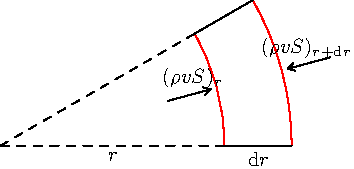
\includegraphics[width=0.8\textwidth]{img/idealfluid/fix_front_shape.pdf}
		\end{figure}
	\end{block}

\end{frame}

\begin{frame}{A Special Wave Equation}
	\begin{outline}
		\1 \emph{continuity equation:}
		$$\pdv{t} (\rho S \dd{r}) = (\rho vS)_r - (\rho v S)_{r+\dd{r}} = -\pdv{(\rho vS)}{r} \dd{r} 
		\quad \to \quad 
		\tikz[baseline]{\node[fill=green!20,anchor=base]{$\displaystyle
			S\pdv{\rho}{t} \approx -\rho_0 \pdv{(vS)}{r}$}}$$
		\1 \emph{Eulerian equation:}
			$$\rho \dv{v}{t} = -\pdv{P}{r} \quad \to \quad 
			\tikz[baseline]{\node[fill=green!20,anchor=base]{$\displaystyle
				\rho_0 \pdv{v}{t} \approx -\pdv{p}{r}$}}$$
		\1 \emph{equation of state:}
		$$P = P(\rho) \quad \to \quad  
		\tikz[baseline]{\node[fill=green!20, anchor=base]{$
		p \approx c_0^2 \rho'$}}$$
		\1 \emph{linear wave equation:}
		$$\tikz[baseline]{\node[fill=red!20,anchor=base]{$\displaystyle
			\qty[\pdv[2]{p}{r}+\pdv{p}{r} \dv{(\ln S)}{r} ]- 
			\frac{1}{c_0^2} \pdv[2]{p}{t}\approx 0$}}$$
	\end{outline}
\end{frame}

\begin{frame}{Special Wave Equations}{Homework}
	\begin{outline}[enumerate]
		\1 Textbook B: 4-5
		\1 Textbook B: 4-6
	\end{outline}
\end{frame}

\section{Plane Waves}
\begin{frame}{Plane Waves}
	\begin{outline}
		\1 1D wave equation
		$$\qty(\pdv[2]{x} - \frac{1}{c_0^2} \pdv[2]{t}) p =0$$
		$$\pdv{p}{\xi}{\eta} = 0, \qty(\xi = c_0t-x, \eta=c_0t+x)$$
		$$\imp\tikz[baseline]{\node[fill=red!20,anchor=base]{$p$}}
		= f(\xi)+g(\eta) \tikz[baseline]{\node[fill=red!20,anchor=base]
			{$= f(c_0t-x) +g(c_0t+x)$}}$$
		\1 Proof
		$$
			\xi = \xi(x,t)\qc \eta = \eta(x,t)
		$$
		$$
			\pdv{\xi} = \qty(\pdv{\xi}{t})^{-1} \pdv{t} + 
			\qty(\pdv{\xi}{x})^{-1} \pdv{x} 
			= \frac{1}{c_0} \pdv{t}-\pdv{x}
		$$
		$$
			\pdv{\eta} = \qty(\pdv{\eta}{t})^{-1} \pdv{t} + 
			\qty(\pdv{\eta}{x})^{-1} \pdv{x} 
			= \frac{1}{c_0} \pdv{t}+\pdv{x}
		$$
		\begin{align*}
			\pdv[2]{}{\xi}{\eta} &= \pdv{\xi}\qty(\pdv{\eta})
			=\pdv{\xi}\qty(\frac{1}{c_0} \pdv{t} + \pdv{x})\\
			&=\qty(\frac{1}{c_0} \pdv{t} - \pdv{x})
			\qty(\frac{1}{c_0} \pdv{t} + \pdv{x})
			= \frac{1}{c_0^2} \pdv[2]{t}- \pdv[2]{x}
		\end{align*}
	\end{outline}
\end{frame}

\begin{frame}{Plane Waves}
	\begin{outline}
		\1 1D wave equation
		$$\qty(\pdv[2]{x} - \frac{1}{c_0^2} \pdv[2]{t}) p =0$$
		$$\imp p = f(c_0t-x) +g(c_0t+x)$$
		\1 \emph{propagating wave} in $x$ direction: \colorbox{red!20}{$p=p(c_0t-x)$}
		\1 (3D wave equation) propagating wave in \emph{unit vector} $\vb{n} = (n_x,n_y,n_z)$ direction 
			$$p=p(c_0t-\vb{n}\vdot \vb{r})$$
		\1 \emph{wave front}: a curved surface where the physical quantites are the same
			$$\zeta = c_0t - \vb{n}\vdot \vb{r} = \text{const.}$$
			$$\dd \zeta = 0 \imp c_0 = \pdv{t} (\vb{n} \vdot \vb{r})$$
		\1 velocity 
		$$\vb{v} = -\frac{1}{\rho_0} \int \grad p \dd{t} =\frac{p}
		{\rho_0c_0}\vb{n}, \quad \qty(\grad p(\zeta) =- \vb{n} 
		\dv{p}{\zeta}, \int p(\zeta) \dd{t} = \frac{1}{c_0} 
		\int p(\zeta)\dd{\zeta})$$
		\end{outline}
\end{frame}

\begin{frame}{Harmonic Plane Wave}
	\begin{outline}
		\1 the \emph{angular frequency}: $\omega$
		$$p(\vb{r},t) = p(\vb{r})\me^{\mj \omega t}\qc(\mj^2 = -1)$$
	\end{outline}
	\begin{alertblock}{Linear Harmonic Wave  Equation (Helmholtz Equation)}
		$$\qty(\laplacian +k^2) p(\vb{r}) = 0$$
		the \emph{wave number}: $k = \omega/c_0$
	\end{alertblock}
	\begin{outline}
		\1 1D wave equation
		$$ \qty(\dv[2]{x}+k^2)p(x) = 0, \imp p(x) =p\st{a} \me^{\mj kx}\qor
		p\st{a}\me^{-\mj kx}$$
		\1 propagating wave with frequency $\omega$
		$$p_\pm(x,t) = p\st{a} \me^{\mj (\omega t\mp kx)}$$
		$$p(\vb{r},t) = p\st{a} \me^{\mj (\omega t- \vb{k}\vdot\vb{r})}
		\qc \qty(\vb{k} = k \vb{n})$$
		\1 particle velocity
		$$v(\vb{r},t) = \vb{n} v\st{a}\me^{\mj (\omega t- \vb{k}
		\vdot\vb{r})}\qc \qty(v\st{a} = \frac{p\st{a}}{\rho_0c_0})$$
	\end{outline}
\end{frame}

\section{Sound Speed}
\begin{frame}{Sound Speed -- the propagating speed of sound waves}
		$$
		c \equiv \sqrt{\dv{P}{\rho}}=\sqrt{\frac{\kappa_s}{\rho}} =
		\sqrt{\frac{1}{\rho\beta_s}}\qc c_0 = c|_{\rho=\rho_0}
		$$
	\begin{outline}
		\1 \emph{incompressible fluids/solids}: $\kappa_s\to \infty\qc \beta_s \to
		0\qc c_0 \to 0$
		\1 \emph{rarefied gas}: $\kappa_s \to 0\qc \beta_s\to \infty\qc
		c_0\to 0$
		\1 \emph{Adiabatic and Ideal Gas}:
		$$P\rho^{-\gamma} = \text{const.} \qor PV^{\gamma} = \text{const.}
		\qc (\gamma\st{air} = 1.4)$$
		$$c = \sqrt{\frac{\gamma P }{\rho}}\qc c_0 = \sqrt{\frac{\gamma P_0}
		{\rho_0}}$$
		\1 \emph{Clapeyron Euation for Ideal Gas}: 
		$$PV = \frac{M}{\mu}RT\qc = P = \frac{\rho}{\mu}RT$$
		$$c_0 = \sqrt{\frac{\gamma}{\mu}RT_0} = c_0|_{T\st{C}=0\celsius}
		\sqrt{1+\frac{T\st{C}}{273}}\approx 331.6 + 0.6T\st{C}\qc(T\st{C}
		=T-273)$$
	\end{outline}
\end{frame}


\begin{frame}{Sound Speed -- the propagating speed of sound waves}
	\begin{outline}
		\1 \emph{Clapeyron Euation for Ideal Gas}: 
		$$PV = \frac{M}{\mu}RT\qc = P = \frac{\rho}{\mu}RT$$
		\2 $P$: the \emph{pressure} of the gas
		\2 $V$: the \emph{volumne} of the gas
		\2 $M$: the \emph{total mass} of the gas (in kilograms)
		\2 $\mu$: the \emph{molar mass} of the gas (in kilograms per mole)
		\2 $R$: the ideal, or universal, \emph{gas constant}, equal
		to the product of the Boltzmann constant and the Avogadro constant
		\2 $T$: the \emph{absolute temperature} of the gass (in Kelvins)
		\2 $\rho$: the \emph{density} of the gass
	\1 Calculate $c_0$ by $T\st{C}$, the \emph{temperature} in Celsius
	$$\tikz[baseline]{\node[fill=red!20,anchor=base]{$c_0$}} =
	\sqrt{\frac{\gamma}{\mu}RT_0} = c_0|_{T\st{C}=0\celsius}
		\sqrt{1+\frac{T\st{C}}{273}}
		\tikz[baseline]{\node[fill=red!20,anchor=base]
			{$\approx 331.6 + 0.6T\st{C}$}}\qc(T\st{C}
		=T-273)$$
	\1 Check for linear assumption in air: $p\st{a} = \SI{0.1}{Pa}\qc 
	T\st{C} = 20 \celsius\qc \rho_0= \SI{1.21}{kg/m^3}$
	$$c_0 \approx \SI{343.6}{m/s}\qc v\st{a} = \frac{p\st{a}}{\rho_0c_0}
	\approx  \num{2.4xe-4}\si{m/s} \ll c_0$$
	\end{outline}
\end{frame}

\begin{frame}{Acoustic impedance, specific acoustic impedance, and 
	characteristic impendace}
	\begin{outline}
		\1 \emph{Acoustic Impedance}: $Z\st{a} = \dfrac{p}{U}$
			\2 lumped parameter system
		\1 \emph{Specific Acoustic Impedance}: $Z\st{s} = \dfrac{p}{v}$
			\2 distributed parameter system
			\2 real part: \emph{specific acoustic resistance}
			\2 imaginary part: \emph{specific acoustic reactance}
		\1 plane wave
			\2 positve direction: $Z\st{s} = \rho_0 c_0$
			\2 negative direction: $ Z\st{s} = -\rho_0c_0$
		\1 \emph{characteristic (specific acoustic) impedance}
			$$z_0 = \rho_0 c_0$$
			\2 represents the acoustic properties of the media
	\end{outline}
\end{frame}

\begin{frame}{Sound Energy}
	\begin{outline}
		\1 consider the fluid particle $\Delta V = \Delta V(\vb{r},t)$
			\2 $t = 0\imp \Delta V_0 = \Delta V(\vb{r},0)\qc P_0\qc \rho_0$
			\1 \emph{kinetic energy}: $$\Delta E\st{k}=\frac12 (\rho_0 
			\Delta V_0)v^2\qc \qty(v = |\vb{v}|)$$
		\1 \emph{potential energy}: the work done by sound pressure $p$
		$$\Delta E\st{p} = -\int_{\Delta V_0}^{\Delta V} p \dd(\Delta V)\approx \Delta V_0 \beta_{s,0} \int_0^p p\dd{p} = \frac12 \beta_{s,0} p^2 \Delta V_0$$
		$$\qty( \dd(\rho \Delta V) = 0 \to \frac{\dd(\Delta V)}{\Delta V_0}   \approx - \frac{\dd{\rho'}}{\rho_0} \xrightarrow{p=c_0^2\rho'} \dd(\Delta V) \approx -\Delta V_0 \beta_{s,0}\dd{p})$$
		\1 \emph{total energy}: $$\Delta E = \Delta E\st{k}+\Delta E\st{p} = \frac12 \qty(\rho_0 v^2+\beta_{s,0}p^2)\Delta V_0$$
	\end{outline}
\end{frame}


\begin{frame}{Sound Energy Density}
	\begin{outline}
		\1 the sound energy per volume (in Pascals)
		$$\eps = \frac{\Delta E}{\Delta V_0}=\frac{\Delta E\st{k}+
			\Delta E\st{p}}{\Delta V_0} = \frac12 \qty(\rho_0 v^2+
			\beta_{s,0}p^2)
		$$
		\1 plane wave: $\Delta E\st{k} = \Delta E\st{p}$
		$$v = \frac{p}{\rho_0c_0} \to \eps = \beta_{s,0}p^2 = 
		\frac{p^2}{\rho_0c_0^2}$$
		\1 \emph{average} of the sound energy density for plane harmonic
		waves
		$$\bar{\eps} = \frac{\overline{p^2}}{\rho_0c_0^2} = \frac{p\st{a}^2}
		{2\rho_0c_0^2} = \frac{p\st{e}^2}{\rho_0c_0^2}\qc
		\qty(\overline{p^2}=\frac12 \qty|p|^2 = p\st{e}^2 = \frac12 p\st{a}^2)
		$$
	\end{outline}
\end{frame}

\section{Sound Power, Sound Intensity}
\begin{frame}{Sound Power, Sound Intensity}
	\begin{outline}
		\1 \emph{sound power} of arbitrary curved surface $\vb{S}$
		(in Watts)
		$$W = \iint_S \vb{v}\vdot \qty(p \dd{\vb{S}}) = \iint_S p \vb{v}
		\vdot \dd{\vb{S}} = \iint_S \vb{I} \vdot \dd{\vb{S}}\qc $$
		\1 \emph{sound energy flux (density)}:
		the rate of energy transfer per unit area 
		($\si{W \cdot m^{-2}}= \si{J \cdot m^{-2}\cdot s^{-1}}$)
		, and \emph{sound intensity}: the time average of it
		$$\vb{I}\equiv p\vb{v}\qc \bar{\vb{I}} = \overline{p\vb{v}}$$
		\1 \emph{complex representations}:
		$$ \vb{I} = \frac12 p\vb{v} +\frac12 p^* \vb{v}\qc 
		\Re(\bar{\vb{I}}) =  \frac12\Re (\overline{p^*\vb{v} +p\vb{v}})$$
		\1 plane sound waves:
		$$\Re(\bar{\vb{I}}) = \frac{1}{\rho_0c_0} \overline{p^2} \vb{n} = 
		\bar{\eps}c_0 \vb{n}$$
		\1 harmonic plane sound waves:
		$$\Re(\bar{\vb{I}} )= \frac12 \Re(p^* \vb{v}) =
		\frac{1}{2\rho_0c_0} |p|^2 \vb{n} = (p\st{e}v\st{e})\vb{n}$$
	\end{outline}
\end{frame}

\begin{frame}{Flux*}
	\begin{outline}
		\1 \emph{Flux}: describes the quantity which passes through
		a surface
	\end{outline}
	\begin{figure}
		\centering
		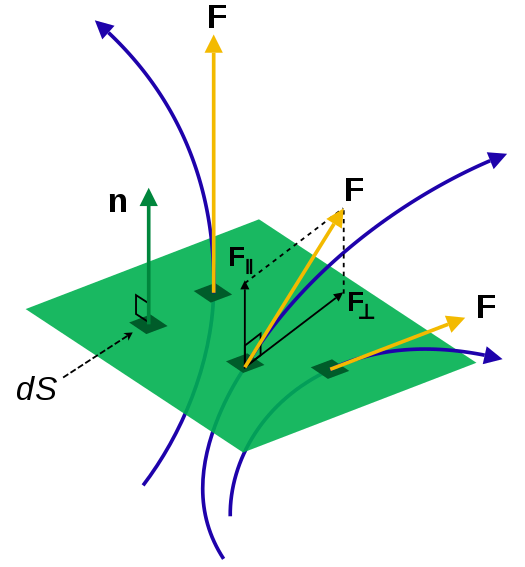
\includegraphics[height=0.6\textheight]{img/idealfluid/General_flux_diagram1.png}
		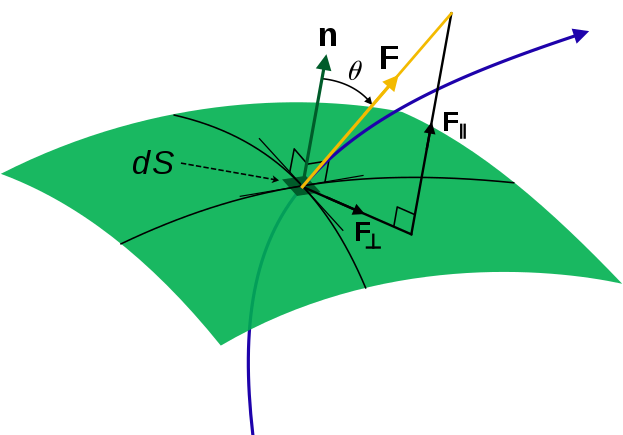
\includegraphics[height=0.4\textheight]{img/idealfluid/General_flux_diagram2.png}
	\end{figure}
\end{frame}

\begin{frame}{Flux*}
	\begin{outline}
		\1 \emph{Flux}: describes the quantity which passes through
		a surface
		\1 \emph{Flux as flow rate per unit area}: $\vb{j}$
			\2 transport phenomena: heat transfer, mass transfer, and
		fluid dynamics
		\2 dimensions: [quantity]$\cdot$[time]$^{-1}\cdot$[area]$^{-1}$
		\2 vector
		\2 also called \emph{flux density}
		\2 $q$: physical quantity that flows
		$$\dv{q}{t} = \iint_S \vb{j} \vdot \dd{\vb{S}}$$
		\1 \emph{Flux as a surface integral}: $\Phi_F$
			\2 electromagnetism, calculus
			\2 dimensions: [quantity]$\cdot$[time]$^{-1}$
			\2 scalar
			$$\Phi_F = \iint_S\vb{F}\vdot \dd{\vb{S}}$$
	\end{outline}
\end{frame}

\section{Sound Pressure Level}
\begin{frame}{Sound Pressure Level, Sound Intensity Level}
	\begin{outline}
	\1 \emph{Sound Pressure Level (SPL)}: a logarithmic measure of the 
	\emph{effective pressure} of a sound relative to a reference value
	$$\mathrm{SPL} \equiv \ln \qty(\frac{p\st{e}}{p\st{ref}} )\si{Np} 
	\equiv 2 \lg \qty(\frac{p\st{e}}{p\st{ref}}) \si{B} 
	\equiv 20 \lg \qty(\frac{p\st{e}}{p\st{ref}}) \si{dB}
	$$
		\2 $p\st{e}$: the \emph{effective sound pressure} or 
		root mean square sound pressure
	\1 $p\st{ref} = 20\mu \si{Pa}$ in air, which is often considered
	as the \emph{threshold of human hearing at $1 \si{kHz}$} 
	(roughly the sound of a 
	mosquito flying 3 m away)
	\1 Examples: $p\st{e} = 1\si{Pa} \imp \mathrm{SPL}=94 \si{dB}\qc 
	p\st{e}\to 2p\st{e} \imp \Delta \mathrm{SPL} = 6 \si{dB}$
	\1 \emph{sound intensity level}
	$$\mathrm{SIL} = 10 \lg \qty(\frac{I}{I\st{ref}} )\si{dB}\qc I\st{ref}
	=\num{10e-12}\si{W\cdot m^2}$$
	\1 relation between the SPL and SIL:
	$$\mathrm{SIL} = \mathrm{SPL} + 10\lg \frac{400}{\rho_0c_0}$$
	\end{outline}
\end{frame}

\begin{frame}{Sound Pressure Level}
	\begin{figure}
		\centering
		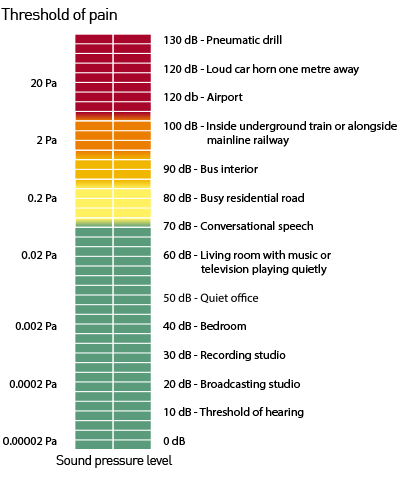
\includegraphics[height=0.9\textheight]{img/idealfluid/spl_table.png}
	\end{figure}
\end{frame}

\subsection{Phon}
\begin{frame}{Phon}

	\begin{block}{Phon}
		The number of phon of a sound is the dB SPL of a sound at a 
		frequency of 1 kHz that sounds just as loud.
	\end{block}

	\begin{outline}
		\1 \emph{loudness}: the subjective perception of sound pressure
			\2 the human hearing sensitivity varies with frequency
		\1 The \emph{phon} is a unit of \emph{loudness} level for \emph{
		pure tones}.
		\1 Its purpose is to compensate for the effect of frequency on the 
		perceived loudness of tones.
		\1 Standards: DIN 45631, ISO 532
	\end{outline}

	\begin{alertblock}{Example}
		60 phons means ``as loud as a 60 dB, 1000 Hz tone''
	\end{alertblock}
\end{frame}

\begin{frame}{Equal Loudness Curve}
	\begin{figure}
		\centering
		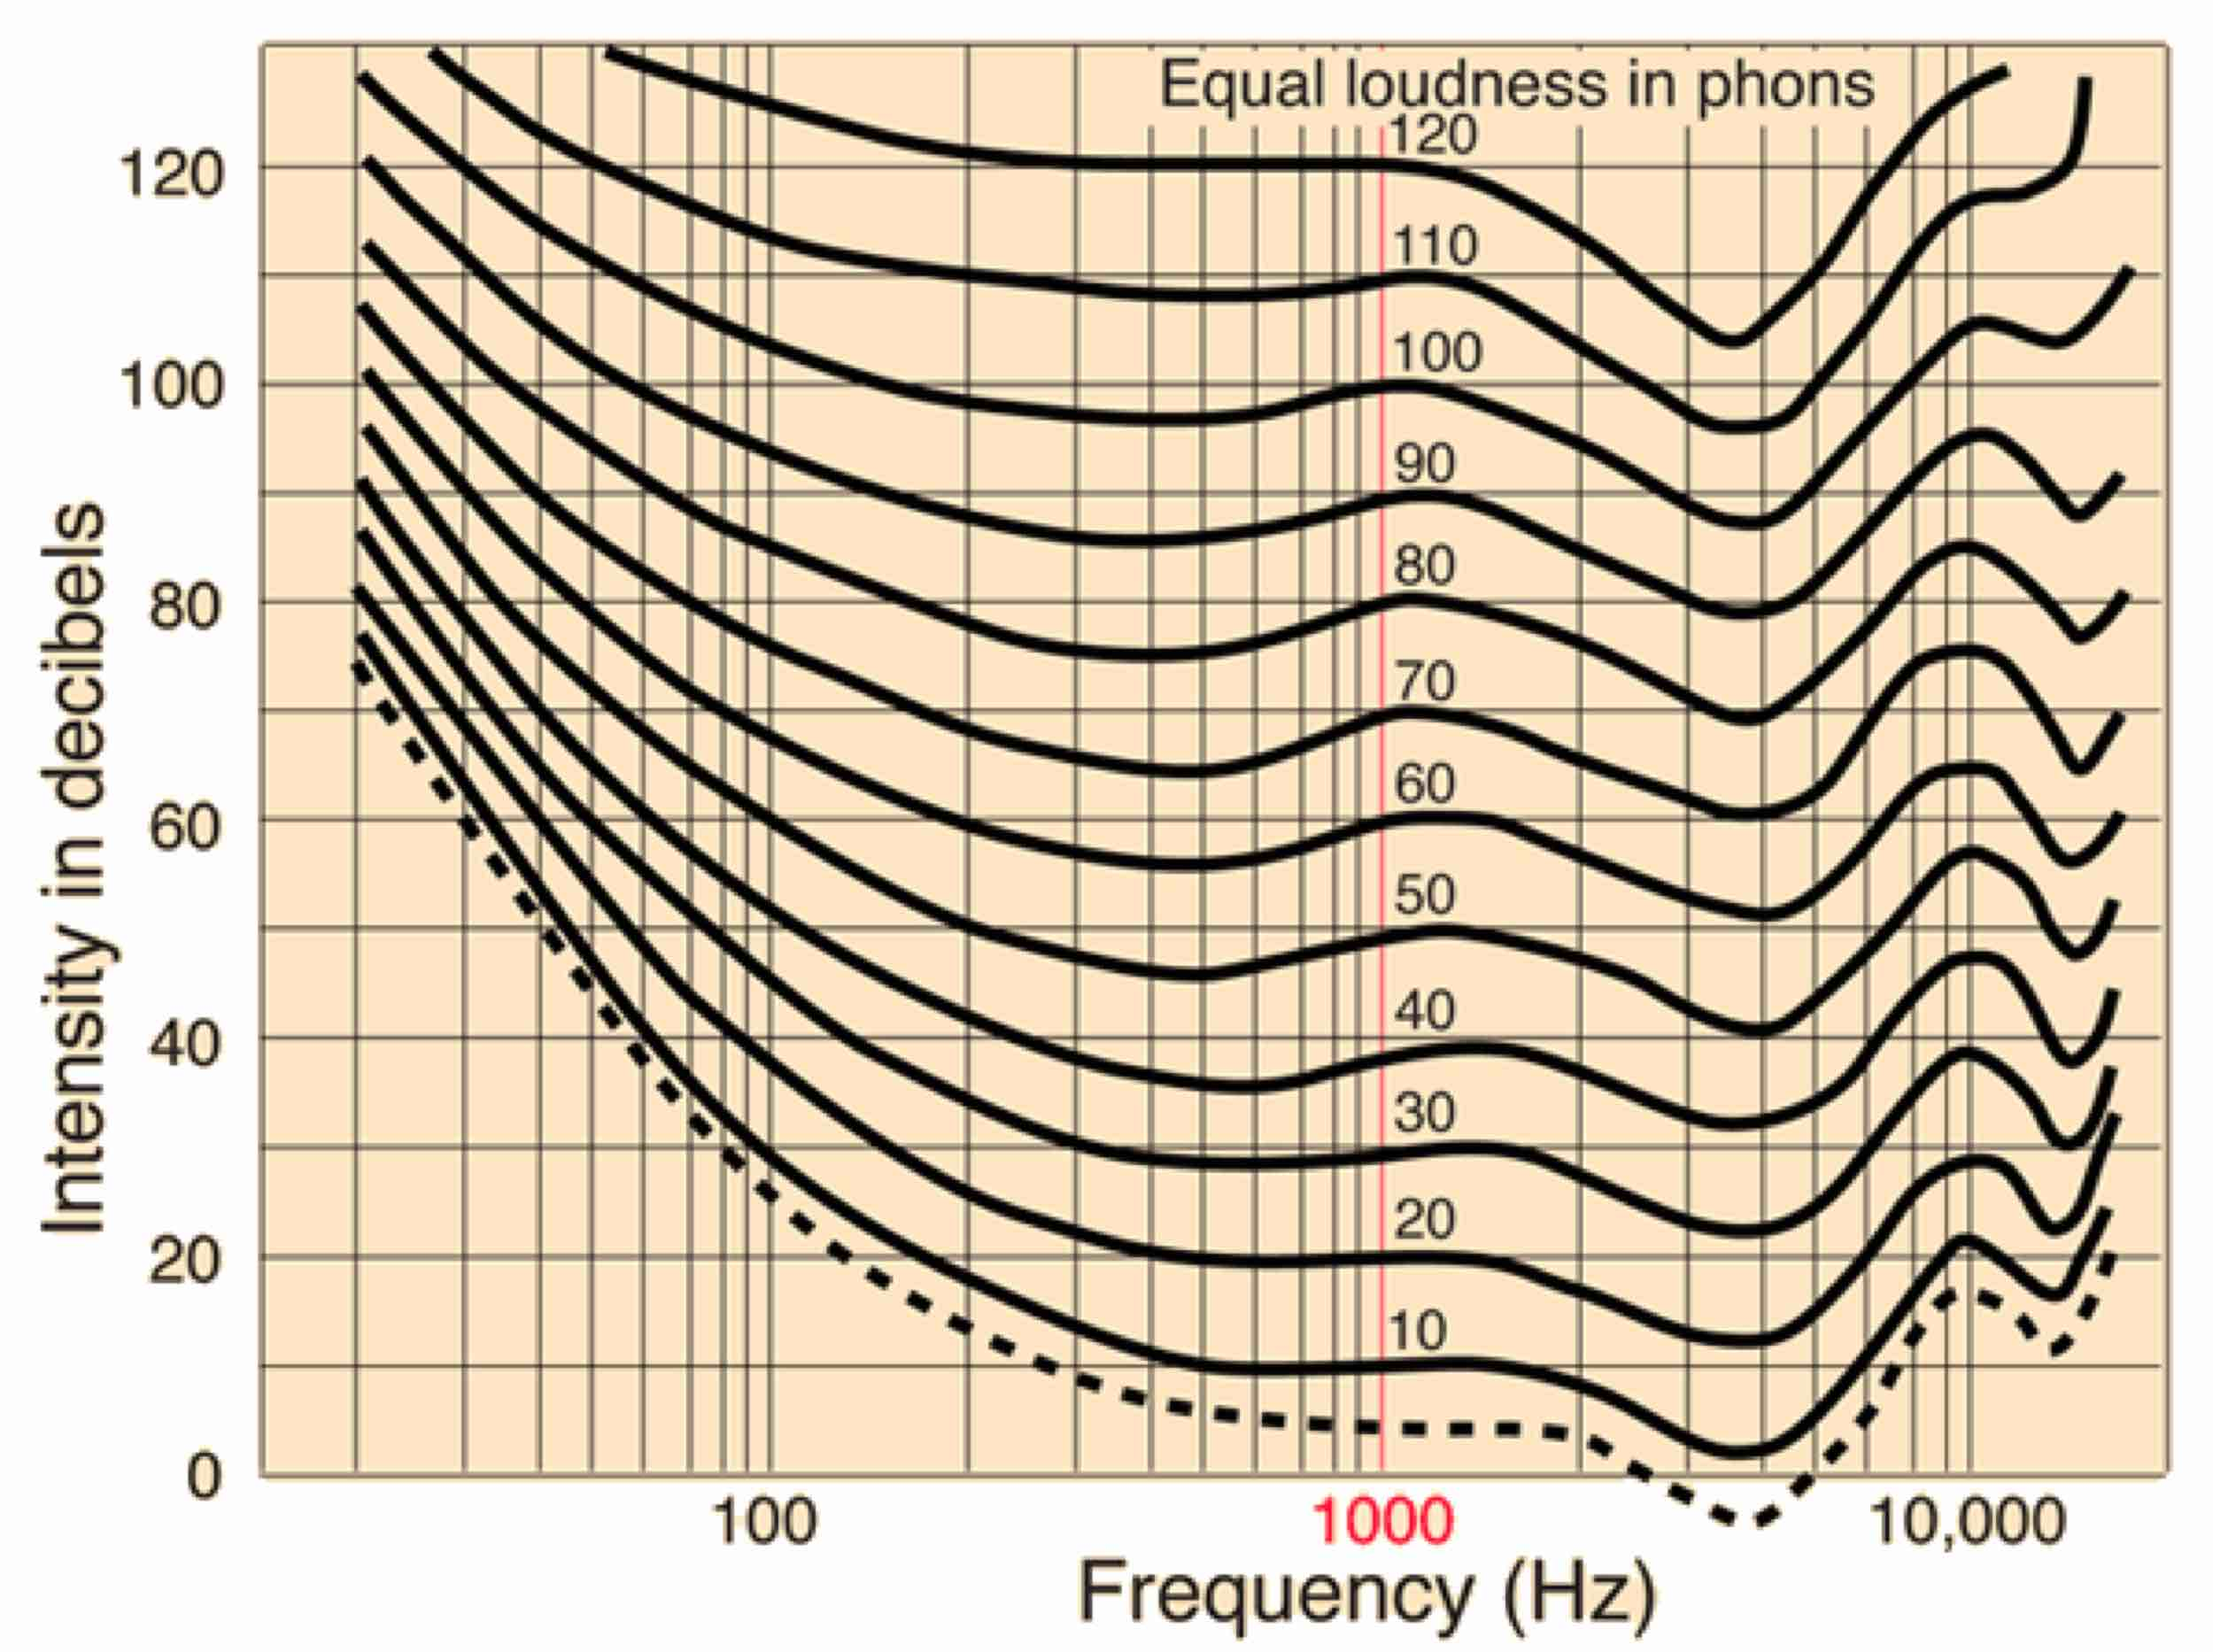
\includegraphics[height=0.85\textheight]{img/idealfluid/eqlou.jpg}
	\end{figure}
\end{frame}

\begin{frame}{Equal Loudness Curve}
	\begin{figure}
		\centering
		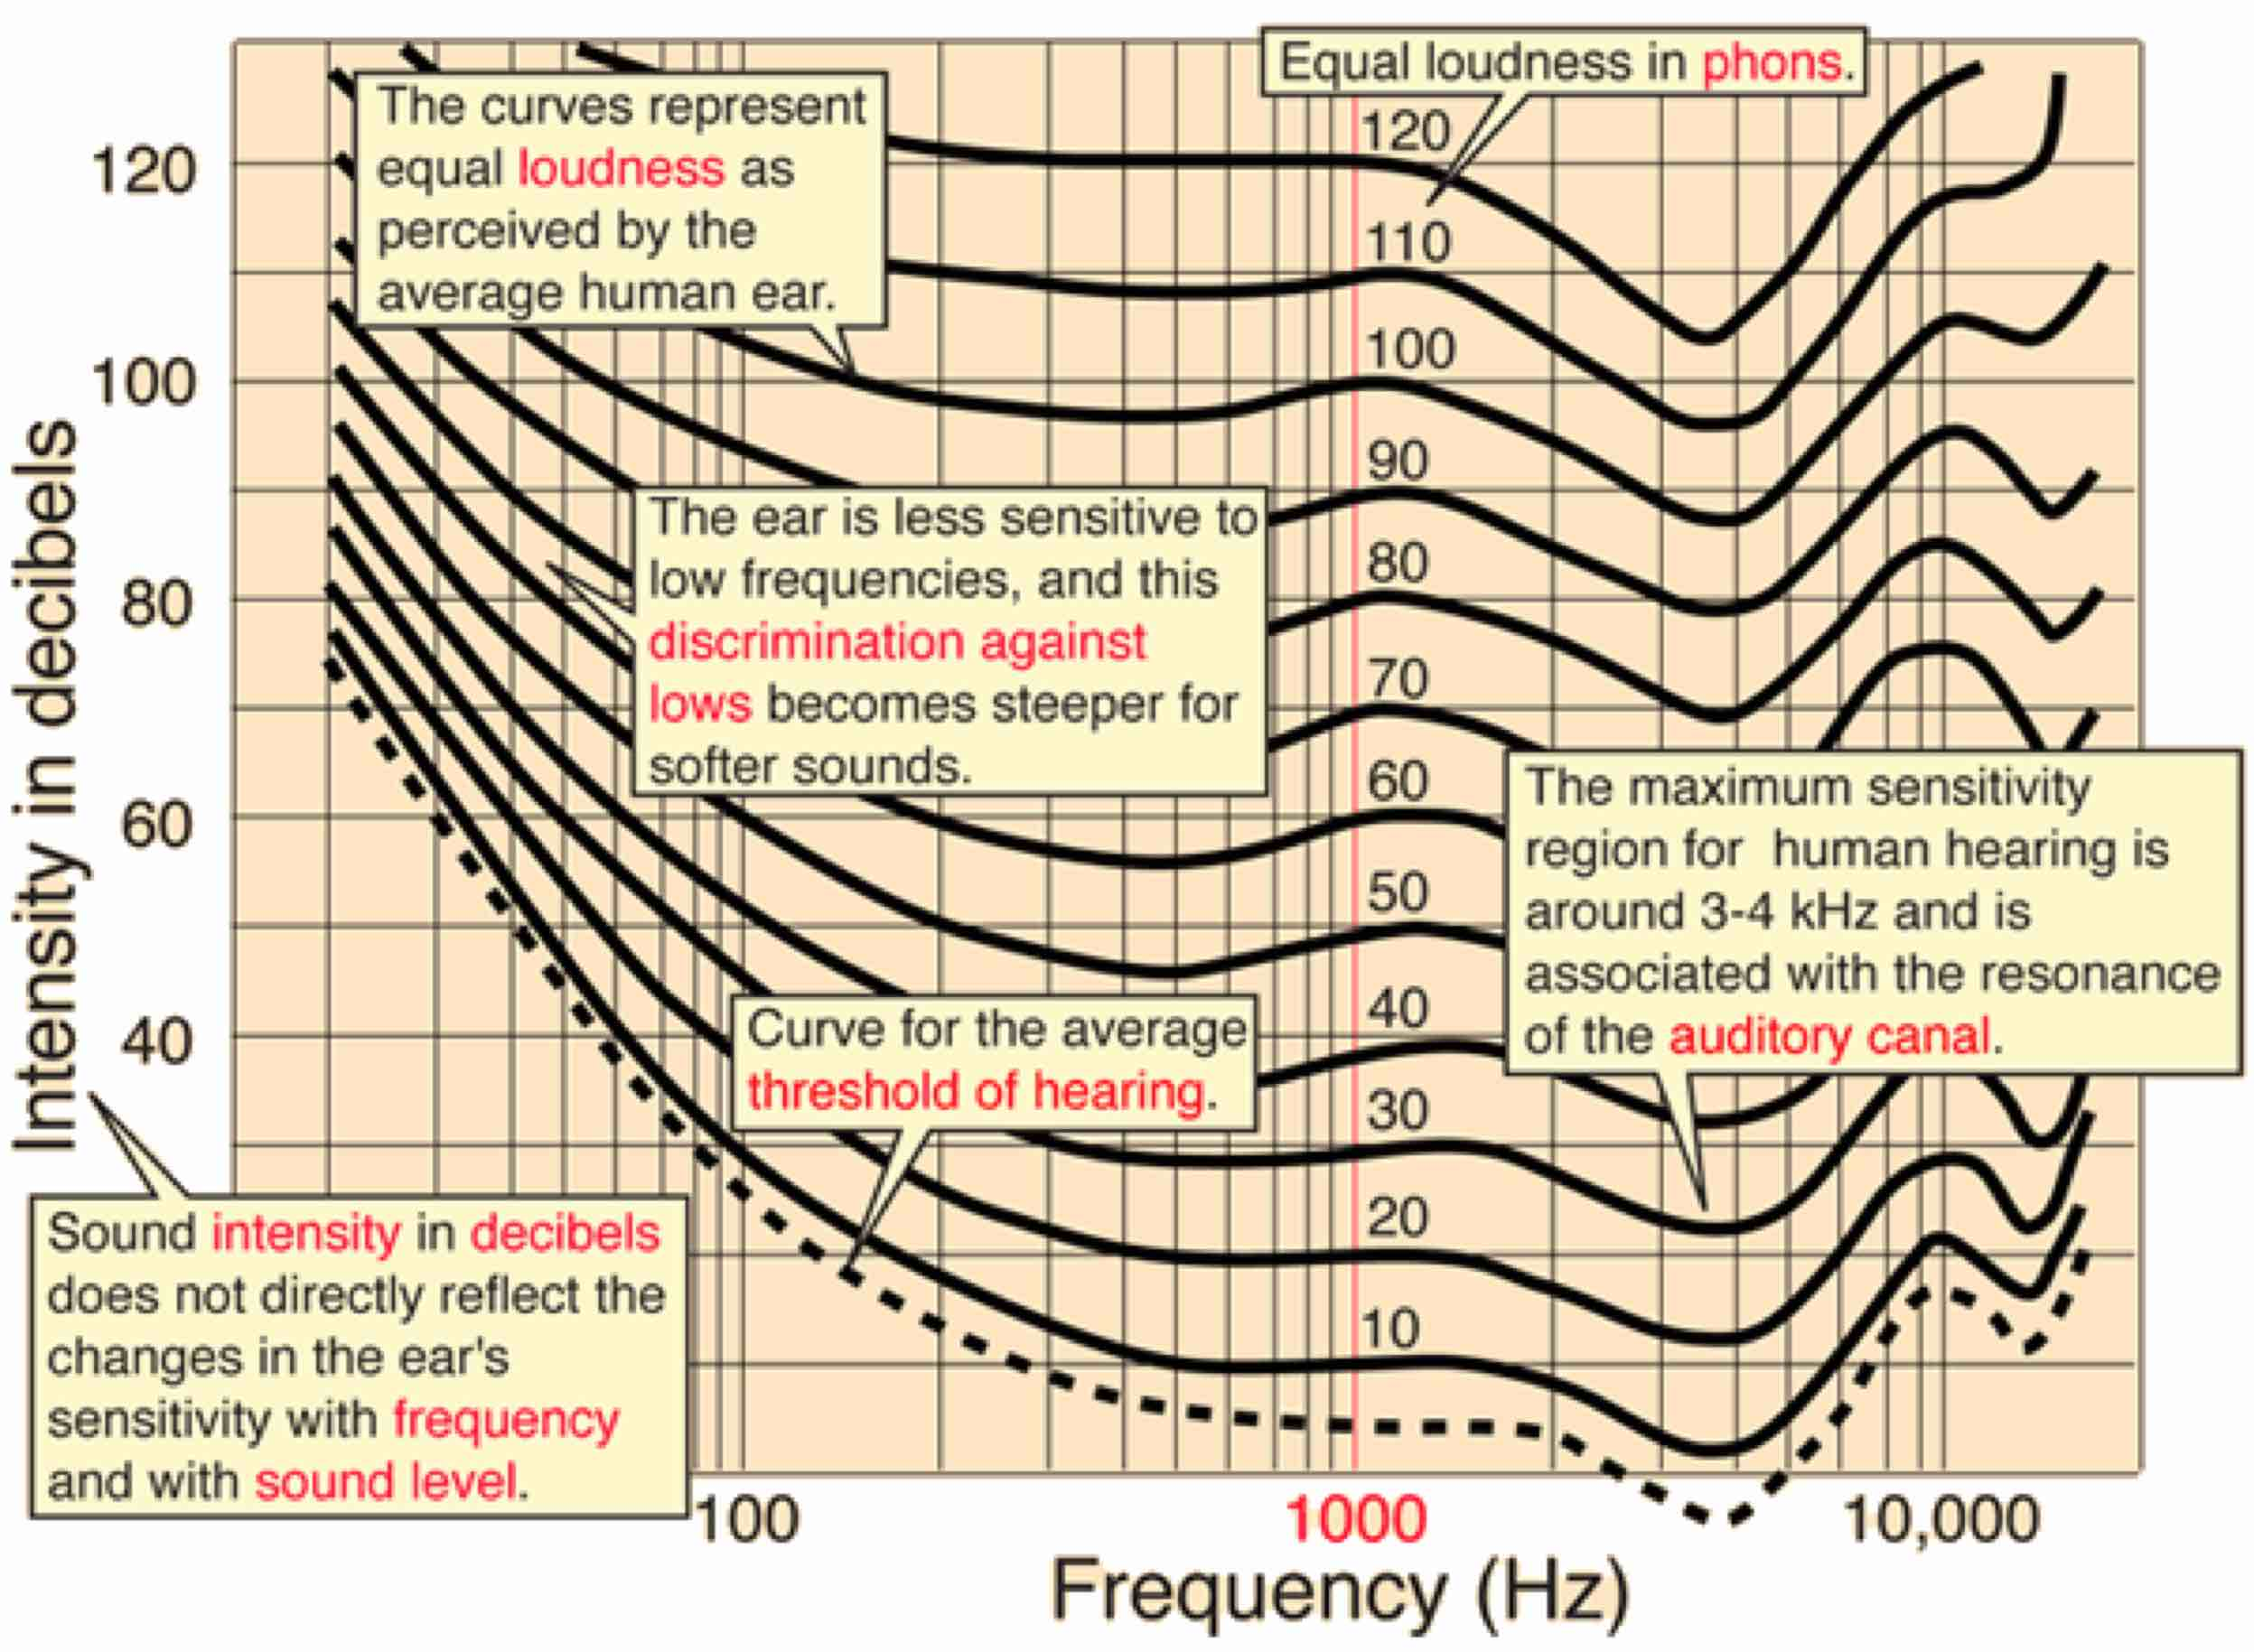
\includegraphics[height=0.85\textheight]{img/idealfluid/eqlou2.jpg}
	\end{figure}
\end{frame}

\begin{frame}{Auditory Canal Resonance}
	$$f_1\approx 3700 \si{Hz}\qc L =\frac{\lambda}{4}\approx 2.3 \si{cm}$$
	$$f_2 = 3f_1 = 13 \si{kHz}$$

	\begin{figure}
		\centering
		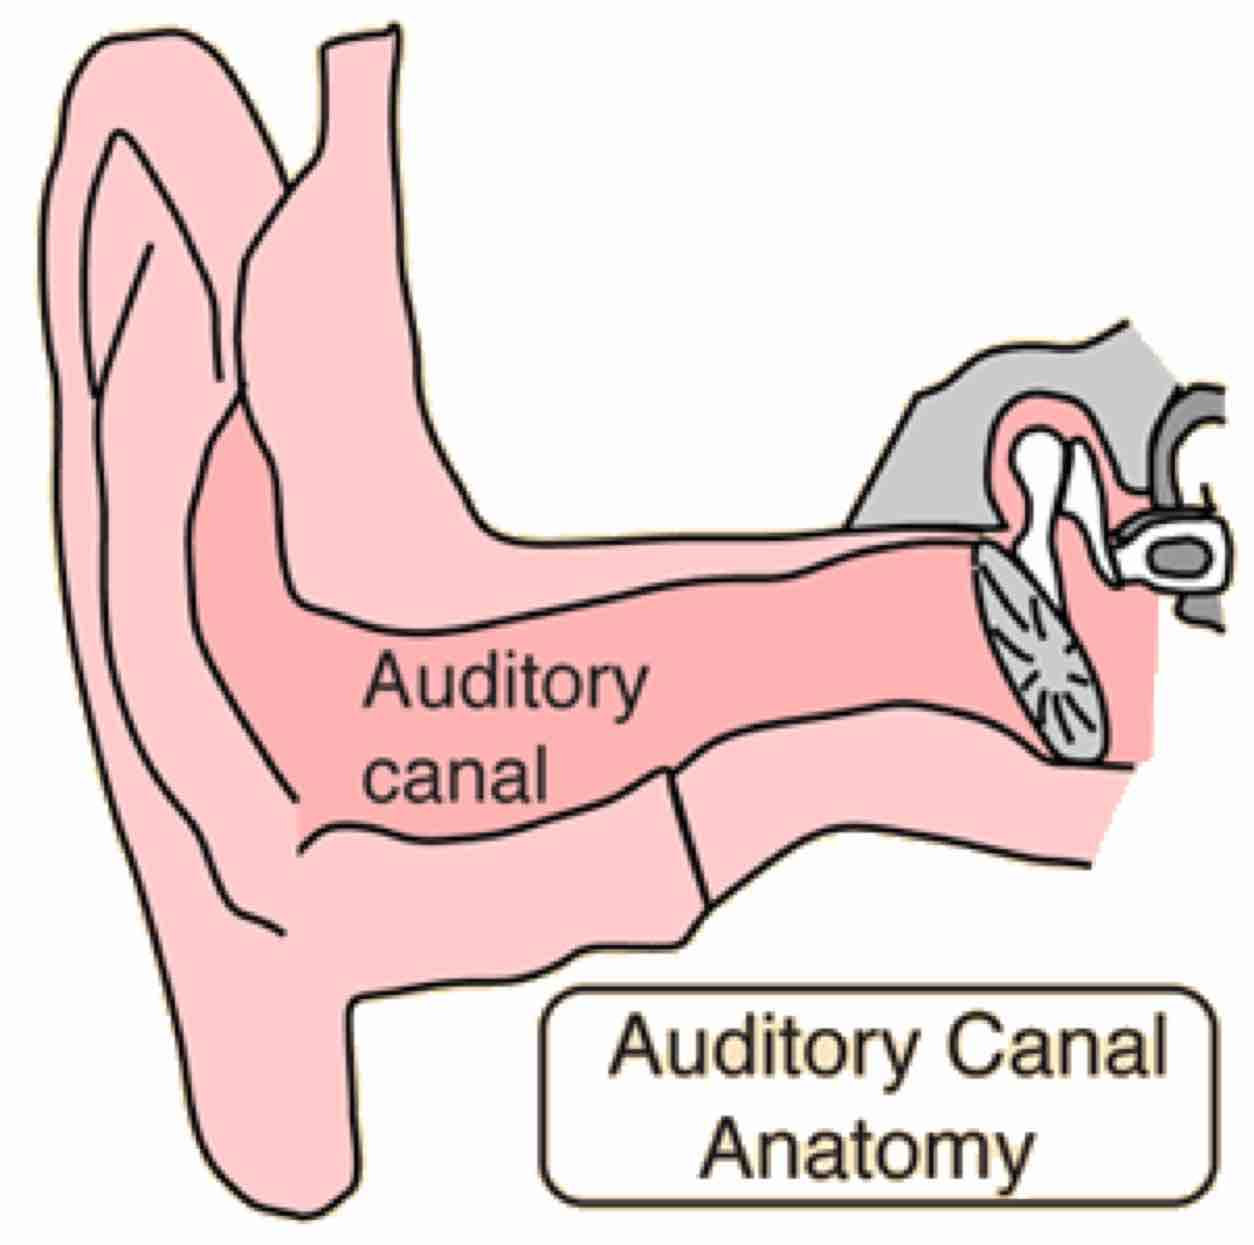
\includegraphics[width=0.3\textwidth]{img/idealfluid/auditory_canal.jpg}
		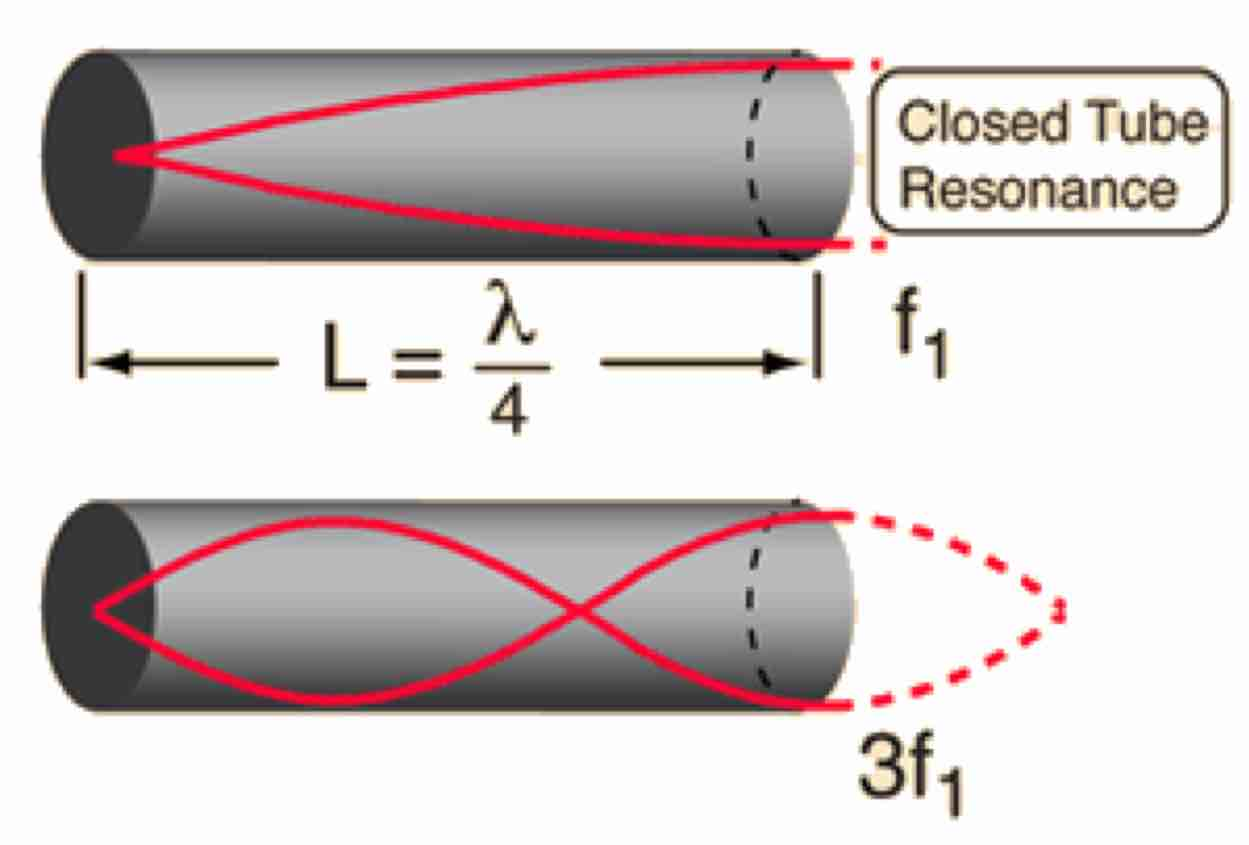
\includegraphics[width=0.3\textwidth]{img/idealfluid/auditory_canal2.jpg}
		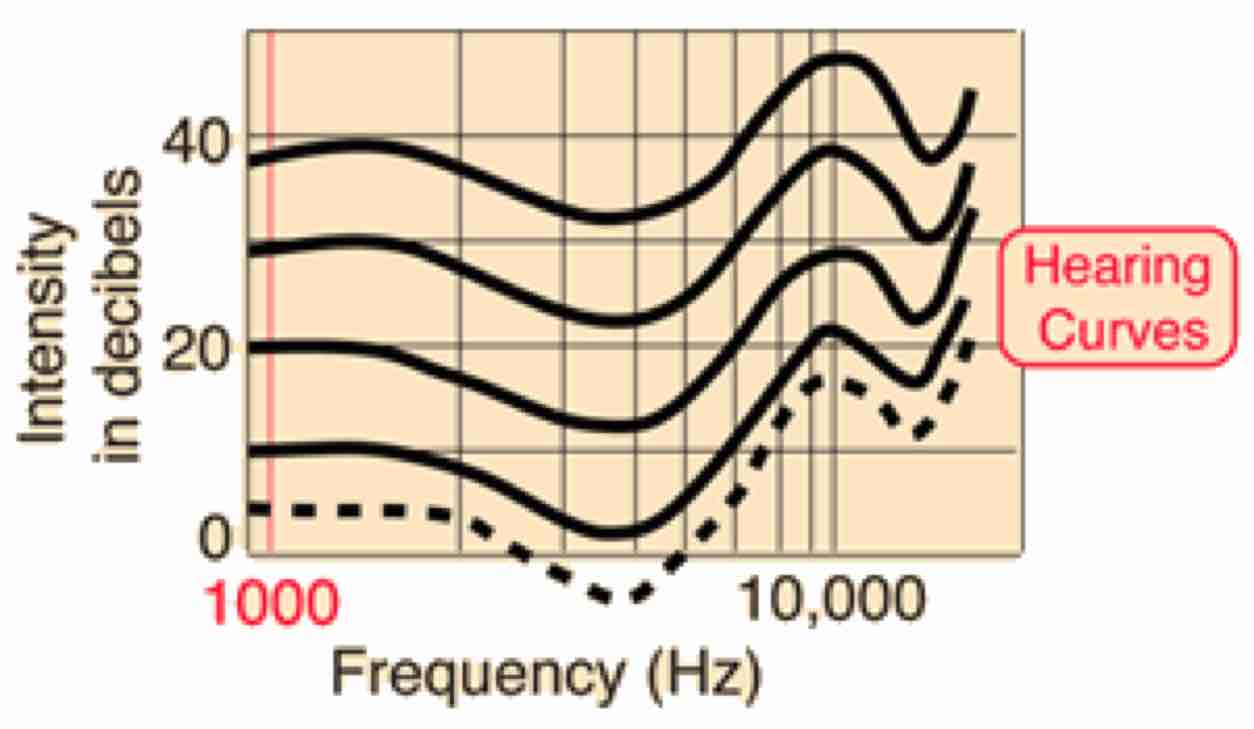
\includegraphics[width=0.3\textwidth]{img/idealfluid/auditory_canal3.jpg}
	\end{figure}
\end{frame}

\begin{frame}{Equal Loudness Curve}
	\begin{figure}
		\centering
		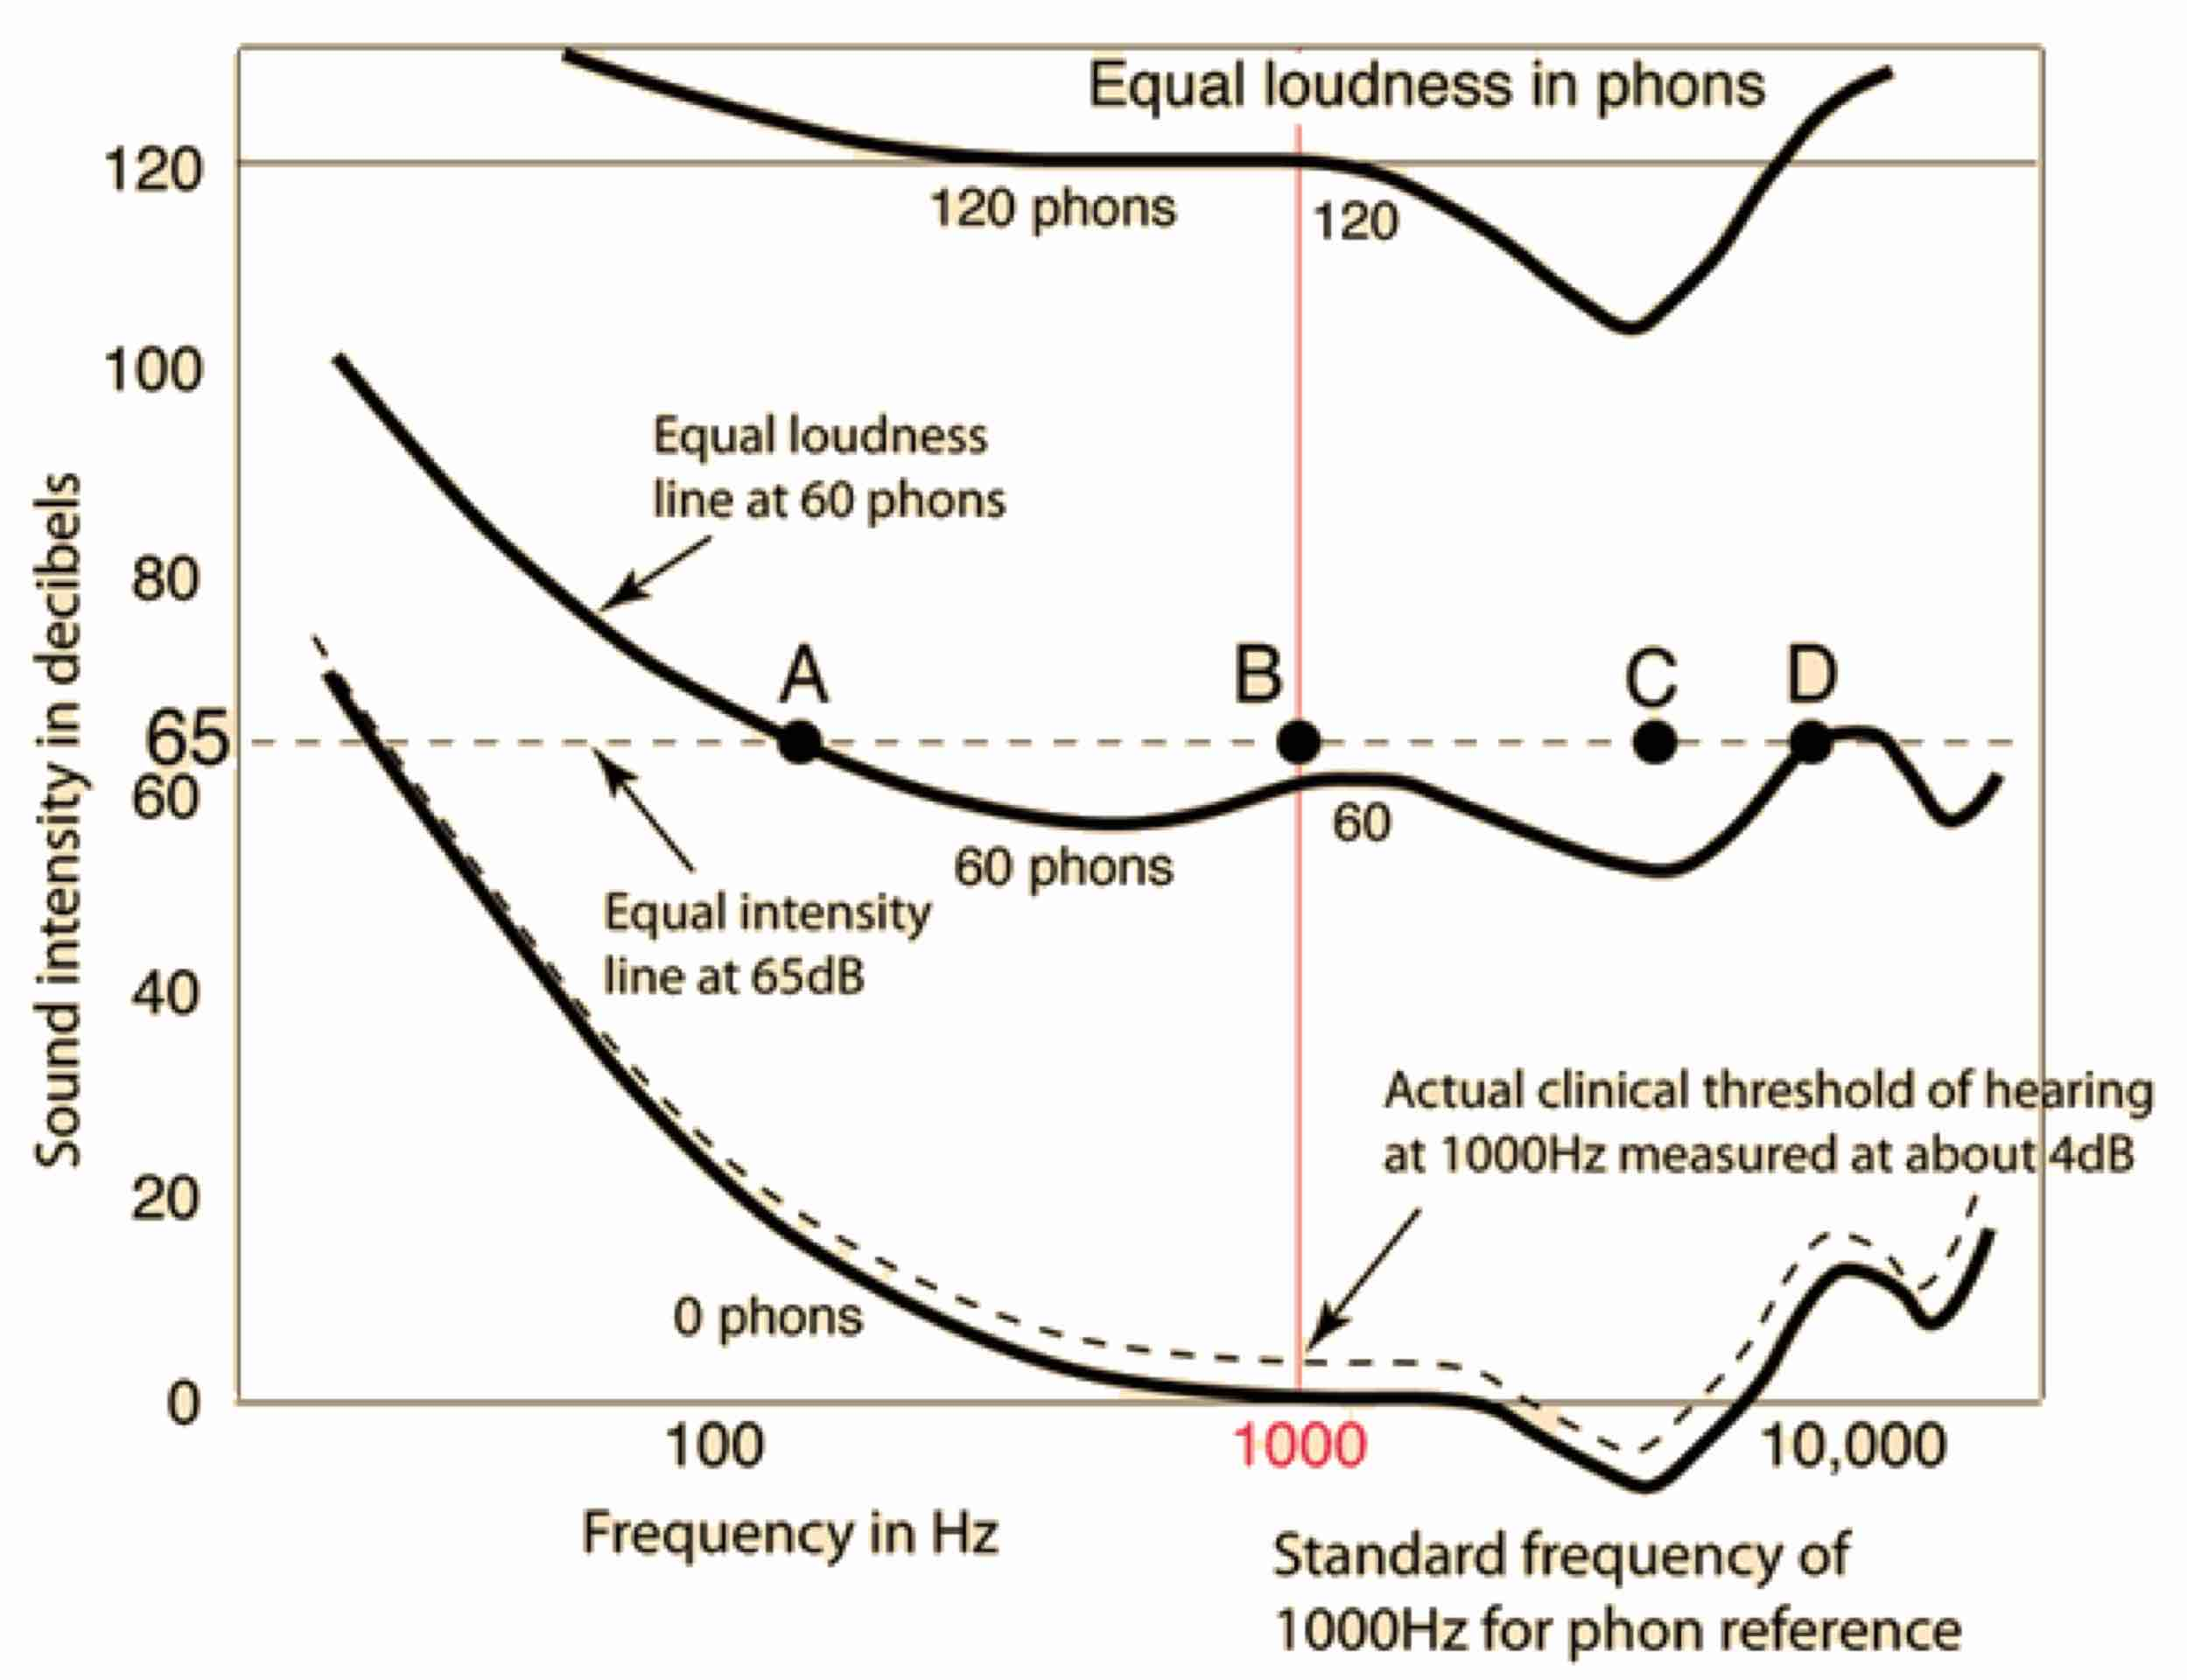
\includegraphics[height=0.85\textheight]{img/idealfluid/eqlou_ex.jpg}
	\end{figure}
\end{frame}

\begin{frame}{Sound Speed, SPL}{Homework}
	\begin{outline}[enumerate]
			\1 Textbook B: 4-7
			\1 Textbook B: 4-10
			\1 Textbook B: 4-12
			\1 Textbook B: 4-13
	\end{outline}
\end{frame}

\section{Plane Waves and Interfaces}
\begin{frame}{Plane Waves and Interfaces}
	\begin{figure}
		\centering
		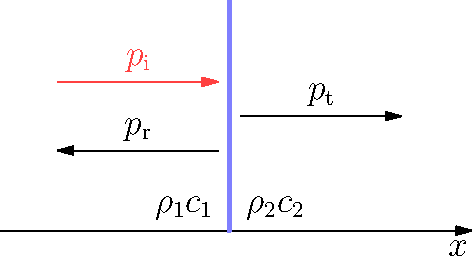
\includegraphics[width=0.45\textwidth]{img/idealfluid/plane_vert_inc.pdf}
	\end{figure}

	\begin{outline}
		\1 \emph{Acoustic interfaces}: the characteristic specific acoustic 
		impedance is different in both sides, $\rho_1c_1$ and $\rho_2c_2$
		\1 \emph{reflection, transmission, and refraction}
		\1 \emph{normal specific acoustic impedance of the interface}
		$$ z\st{n}= \frac{p}{\vb{v}\vdot \vb{n}}$$
		\1 continuous boundary conditions 
			\2 sound pressure: $p_1 =p_2$
			\2 normal velocity: $\vb{v}_1\vdot \vb{n} = \vb{v}_2 \vdot \vb{n}$
			\2 normal specific acoustic impedance: $z\st{n1} = z\st{n2}$
	\end{outline}
\end{frame}

\section{Normal Incidence}
\subsection{Reflection and Transmission Coefficients}
\begin{frame}{Normal Incidence: Reflection and Transmission Coefficients}
	\begin{outline}
		\1 Incident field
		$$
		\begin{cases}
			p\st{i} = p\st{ia}\me^{\mj(\omega t-k_1 x)}\\
			v\st{i} = v\st{ia} \me^{\mj (\omega t - k_1 x)}
		\end{cases}
		\qc \qty(v\st{ia} = \frac{p\st{ia}}{z_1}\qc z_1 = \rho_1 c_1)
		$$
		\1 Reflective field
		$$
		\begin{cases}
			p\st{r} = p\st{ra}\me^{\mj(\omega t+k_1 x)}\\
			v\st{r} = v\st{ra} \me^{\mj (\omega t + k_1 x)}
		\end{cases}
		\qc \qty(v\st{ra} = -\frac{p\st{ra}}{z_1})
		$$
		\1 Transmissive field
		$$
		\begin{cases}
			p\st{t} = p\st{ta}\me^{\mj(\omega t-k_2 x)}\\
			v\st{t} = v\st{ta} \me^{\mj (\omega t - k_2 x)}
		\end{cases}
		\qc \qty(v\st{ta} = \frac{p\st{ta}}{z_2}\qc z_2 = \rho_2c_2)
		$$
		\1 Boundary conditions at $x=0$:
		$
		\begin{cases}
			p\st{i} +p\st{r} = p\st{t}\\
			v\st{i} +v\st{r} = v\st{t}
		\end{cases}
		\qc \qty(z_{12} = \dfrac{z_2}{z_1})
		$
		$$
		\imp
		\begin{cases}
		r_p \equiv \dfrac{p\st{ra}}{p\st{ia}} =\dfrac{z_2-z_1}{z_2+z_1} = 
		\dfrac{z_{12}-1}{z_{12}+1}
		\qc r_v \equiv \dfrac{v\st{ra}}{v\st{ia}} = -r_p\\
		t_p \equiv \dfrac{p\st{ta}}{p\st{ia}} =\dfrac{2z_2}{z_1+z_2} = \dfrac{2z_{12}
	}{1+z_{12}}
	\qc t_v \equiv \dfrac{v\st{ta}}{v\st{ia}} = \dfrac{2z_1}{z_1+z_2}
	=\dfrac{2}{1+z_{12}}
		\end{cases}
		$$
	\end{outline}
\end{frame}

\subsection{Sound Hard and Sound Soft Boundaries}

\begin{frame}{Sound Hard and Sound Soft Boundaries}
	\begin{outline}
		\1 \emph{Impedance Matching}: $z_2=z_1$
			$$r_p = r_v = 0\qc t_p = t_v = 1$$
		\1 \emph{Sound Hard Boundary}: $z_2>z_1$
		$$0<r_p<1\qc -1<r_v<0\qc 1<t_p<2\qc 0<t_v<1$$
			\2 \emph{very hard}: $z_2>>z_1$
			$$r_p \approx 1\qc r_v \approx -1\qc t_p \approx 2\qc t_v\approx 0$$
		\1 \emph{Sound Soft Boundary}: $z_2<z_1$
		$$-1<r_p<0\qc 0<r_v<1\qc 0<t_p<1\qc 1<t_v<2$$
			\2 \emph{very soft}: $z_2<<z_1$
			$$r_p\approx -1\qc r_v \approx 1\qc t_p \approx0\qc t_v\approx 2$$
	\end{outline}
\end{frame}

\subsection{Sound Intensity}
\begin{frame}{Reflection and Transmission Coefficients of Sound Intensity}
	\begin{outline}
		\1 sound intensity: 
		$
		\vb{I}\st{i} = I\st{i} \vb{n}\st{i}\qc
		\vb{I}\st{r} = I\st{r} \vb{n}\st{r}\qc
		\vb{I}\st{t} = I\st{t} \vb{n}\st{t}
		$
		\1 conditions: \emph{plane wave} and \emph{harmonic}
		$$\vb{I}\st{i} = \frac12 \Re (p^* \vb{v}\st{i}) 
		=\frac{|p\st{i}|^2}{2z_1}\vb{n}\st{i}
		$$
		\1 reflection coefficient
		$$r_I \equiv \frac{||\vb{I}\st{r}||}{||\vb{I}\st{i}||} 
		= \frac{I\st{r}}{I\st{i}}
		= \frac{|p\st{r}|^2}{2z_1}
		\bigg/ \frac{|p\st{i}|^2}{2z_1} 
		=\frac{|p\st{ra}|^2}{|p\st{ia}|^2}
		= |r_p|^2 
		= \qty(\frac{z_1-z_2}{z_1+z_2})^2 $$
		\1 transmission coefficient
		$$t_I \equiv \frac{||\vb{I}\st{t}||}{||\vb{I}\st{i}||}
		= \frac{I\st{t}}{I\st{i}}
		= \frac{|p\st{t}|^2}{2z_2}
		\bigg/ \frac{|p\st{i}|^2}{2z_1} 
		= z_{21} \frac{|p\st{ra}|^2}{|p\st{ia}|^2}
		= z_{21} |t_p|^2 
		= \frac{4z_1z_2}{(z_1+z_2)^2}$$
		\1 Conservation of sound energy
		$$r_I+t_I = 1$$
	\end{outline}
\end{frame}

\subsection{Normal Specific Acoustic Impedance of the Interface}
\begin{frame}{Application of $z\st{n}$}
	\begin{outline}
		\1 \emph{Normal specific acoustic impedance of the interface} at
		$x$: $z\st{n}(x)$
		$$z\st{n}(x=0) = \left. \frac{p\st{i}+p\st{r}}{v\st{i} +v\st{r}}\right|
		_{x=0} = z_1 \frac{1+r_p}{1-r_p}$$
		$$\imp \quad r_p = \frac{z\st{n}(0) - z_1}{z\st{n}(0)+z_1}$$
		\1 at the transmission side: $z\st{n}(x=0) = z_2$
		$$\imp \quad r_p = \frac{z_2-z_1}{z_2+z_1}$$
		\1 \emph{OR} at the transmission side: $$z\st{n}(x=0) = 
		z_2\dfrac{z_1+\mj z_2 \tan k_2d}{z_2+\mj z_1\tan k_2 d}$$
		$$\imp \quad r_p = \mj \frac{(z_2^2-z_1^2)\tan k_2d}{2
		z_1z_2 + \mj (z_1^2+z_2^2)\tan k_2 d}$$
			\2 the reflection coefficient when the interlayer is presented
	\end{outline}
\end{frame}

\subsection{Homework}
\begin{frame}{Normal Incidence}{Homework}
	\begin{outline}[enumerate]
			\1 Textbook B: 4-15
			\1 Textbook B: 4-16
	\end{outline}
\end{frame}

\section{Oblique Incidence}

\begin{frame}{Oblique Incidence}{reflection and transmission coefficients}
	\begin{columns}
		\column{0.6\textwidth}
		\begin{outline}
			\1 sound field
			$$\begin{cases}p\st{i} = p\st{ia} \me^{\mj (\omega t-\vb{k}\st{i}
				\vdot \vb{r})} \\ \vb{v}\st{i} = \dfrac{p\st{i}}{z_1}\vb{n}\st{i}\end{cases}
			, \qty[\begin{split}\vb{k}\st{i} &= k_1\vb{n}\st{i}\\ \vb{n} &=
				(\cos \theta\st{i}, \sin\theta\st{i})\end{split}]$$
			$$\begin{cases}p\st{r} = p\st{ra} \me^{\mj (\omega t-\vb{k}\st{r}
				\vdot \vb{r})} \\ \vb{v}\st{r} = \dfrac{p\st{r}}{z_1}\vb{n}\st{r}\end{cases}
			, \qty[\begin{split}\vb{k}\st{r} &= k_1\vb{n}\st{r}\\ \vb{n} &=
				(-\cos \theta\st{r}, \sin\theta\st{r})\end{split}]$$
			$$\begin{cases}p\st{t} = p\st{ta} \me^{\mj (\omega t-\vb{k}\st{t}
				\vdot \vb{t})} \\ \vb{v}\st{t} = \dfrac{p\st{t}}{z_2}\vb{n}\st{t}\end{cases}
			, \qty[\begin{split}\vb{k}\st{t} &= k_2\vb{n}\st{t}\\ \vb{n} &=
				(\cos \theta\st{t}, \sin\theta\st{t})\end{split}]$$
		\end{outline}
		\column{0.4\textwidth}
		\begin{figure}
			\centering
			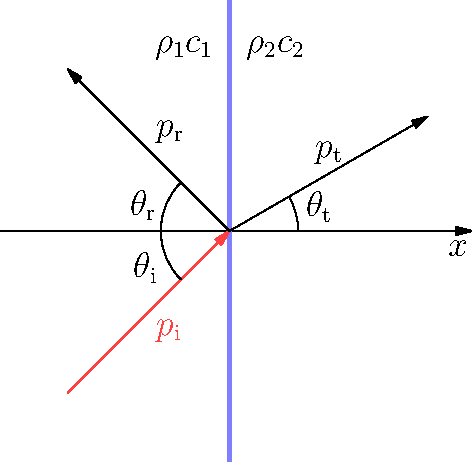
\includegraphics[width=\textwidth]{img/idealfluid/planeObliqueIncidence.pdf}
		\end{figure}
	\end{columns}

	\begin{outline}
		\1 boundary conditions at $x=0$:
		$$\begin{cases} p\st{i} +p\st{r} = p\st{t} \\
			\vb{v}\st{i} +\vb{v} \st{r} =\vb{v}\st{t} \Leftrightarrow
			v_{\text{i}, x} + v_{\text{r}, x} = v_{\text{t}, x} \qand
			v_{\text{i}, y} + v_{\text{r}, y} = v_{\text{t}, y}
		\end{cases}
			$$
		% \1 in region 1
		% $$p_1 \equiv p\st{i} +p\st{r} = p\st{ia} \me^{\mj (\omega t
			% -\vb{k}\st{i}\vdot \vb{r})} + p\st{ra} \me^{\mj (\omega t
			% -\vb{k}\st{r}\vdot \vb{r})} $$
			% $$\vb{v}_{1,x} \equiv \vb{v}_1 \vdot \vb{e}_s = 
			% (\vb{v}\st{i} +\vb{v}\st{r})\vdot \vb{e}_x
			% = \dfrac{p\st{i}}{z\st{ni}} + \frac{p\st{r}}{z\st{nr}}
			% $$
			% $$\qty(z\st{ni} = \frac{z_1}{\cos \theta\st{i}}
			% \qc z\st{nr} = -\frac{z_1}{\cos \theta\st{r}})$$
	\end{outline}
\end{frame}

\begin{frame}{Oblique Incidence}{Snell's Law}
	\begin{outline}
		\1 boundary conditions at $x=0$
		$$
		\begin{cases}
			\displaystyle
			p\st{ia} \me^{-\mj k_1 \sin \theta\st{i} y} +
			p\st{ra} \me^{-\mj k_1 \sin \theta\st{r} y} =
			p\st{ta} \me^{-\mj k_2 \sin \theta\st{t} y}\\
			\displaystyle
			\frac{p\st{ia}}{z\st{ni}} \me^{-\mj k_1 \sin \theta\st{i} y} +
			\frac{p\st{ra}}{z\st{nr}} \me^{-\mj k_1 \sin \theta\st{r} y} =
			\frac{p\st{ta}}{z\st{nt}} \me^{-\mj k_2 \sin \theta\st{t} y}
		\end{cases}
		$$
		$$
			\qty(z\st{ni} = \frac{z_1}{\cos \theta\st{i}}
			\qc z\st{nr} = -\frac{z_1}{\cos \theta\st{r}}
			\qc z\st{nt} = \frac{z_2}{\cos \theta\st{t}})
		$$
		\1 to satisfy the equations, we have (\emph{Snell's Law})
		$$
		k_1 \sin \theta\st{i} = k_1\sin\theta\st{r} = k_2\sin\theta\st{t}
		\imp
		\begin{cases}
			\displaystyle
			\theta\st{i} = \theta\st{r}\\
			\displaystyle
			n = \frac{\sin \theta\st{i}}{\sin \theta\st{t}} = 
			\frac{k_2}{k_1} = \frac{c_1}{c_2}
		\end{cases}
		$$
		\2 incident angle = reflection angle
		\1 $n$: \emph{refraction index}
	\end{outline}
\end{frame}

\begin{frame}{Oblique Incidence}{reflection and transmission coefficients}
	\begin{outline}
		\1 the boundary conditions s.t. Snell's law:
		$$ 
		\begin{cases}
			p_\text{ia}+p_\text{ra}=p_\text{ta}\\
			\displaystyle \frac{p_\text{ia} - p\st{ra}}{z_\text{n1}} = 
			\frac{p\st{ta}}{z_\text{n2}}
		\end{cases}	
		\imp 
		\begin{cases}
			1+r\st{p}=t\st{p}\\
			\displaystyle \frac{1-r\st{p}}{z_\text{n1}} = \frac{t\st{p}}{z_\text{n2}}
		\end{cases}	
		\qc
		\qty(
		\begin{matrix}
			z_\text{n1}\equiv z\st{ni}=-z\st{nr}\\
			z_\text{n2}\equiv z\st{nt}
		\end{matrix}	
		)
		$$
		\1 the ratio of density: $m\equiv \rho_2/\rho_1$, refractive index: $n=k_2/k_1=c_1/c_2$
		\1 reflection and transmission coeff.:
		$$
		r_p\equiv\frac{p\st{ra}}{p\st{ia}} = \frac{z_\text{n2}-z_\text{n1}}{z_\text{n2}+z_\text{n1}} = \frac{R_2\cos\theta\st{i}-R_1\cos\theta\st{t}}{R_2\cos\theta\st{i}+R_1\cos\theta\st{t}}=\frac{m\cos\theta\st{i}-
		\sqrt{n^2-\sin^2\theta\st{i}}}{m\cos\theta\st{i}
		+\sqrt{n^2-\sin^2\theta\st{i}}}
		$$
		$$
		t_p\equiv\frac{p\st{ta}}{p\st{ia}} = 
		\frac{2z_\text{n2}}{z_\text{n2}+z_\text{n1}} = 
		\frac{2R_2\cos\theta\st{i}}{R_2\cos\theta\st{i}+
		R_1\cos\theta\st{t}}=\frac{2m\cos\theta\st{i}}{m\cos\theta\st{i}+
		\sqrt{n^2-\sin^2\theta\st{i}}}
		$$
	\end{outline}
\end{frame}

\subsection{Sound Intensity}
\begin{frame}{Oblique Incidenc}{Sound Intensity and Conservation of Energy}
	\begin{outline}
		\1 sound intensity: 
		$
		\vb{I}\st{i} = I\st{i} \vb{n}\st{i}\qc
		\vb{I}\st{r} = I\st{r} \vb{n}\st{r}\qc
		\vb{I}\st{t} = I\st{t} \vb{n}\st{t}
		$
		$$
		I\st{i} = \frac{|p\st{i}|^2}{2z_1}\qc
		I\st{r} = \frac{|p\st{r}|^2}{2z_1}= I\st{i} |r_p|^2\qc
		I\st{t} = \frac{|p\st{t}|^2}{2z_2} = z_{21} I\st{i} |t_p|^2
		$$
		\1 in the surface direction (normal): $I\st{n} = \vb{I}\vdot \vb{n}$
		$$
		I\st{i,n} = I\st{i} \cos \theta\st{i} \qc
		I\st{r,n} = -I\st{i} |r_p|^2 \cos \theta\st{i} \qc
		I\st{t,n} = z_{21} I\st{i}|t_p|^2 \cos \theta\st{t}
		$$
		\1 conservation of energy
		$$
		I\st{i,n} = I\st{r,n} + I\st{t,n}
		\Leftrightarrow
		\vb{I}\st{i} \vdot \vb{S} =(\vb{I}\st{r}+
		\vb{I}\st{t}) \vdot \vb{S}\qc (\vb{S} = \vb{n} S)
		$$
		\1 \emph{normal} reflection and transmission coefficients
		$$
		r_{I, \mathrm{n}} = \frac{I\st{r,n}}{I\st{i,n}} = 
		-|r_p|^2 = - \qty|\frac{z\st{n2}-z\st{n1}}{z\st{n2}+z\st{n1}}|^2$$
		$$
		t_{I, \mathrm{n}} = \frac{I\st{t,n}}{I\st{i,n}} =
		\frac{4z\st{n1}z\st{n2}}{|z\st{n1}+z\st{n2}|^2}
		$$
		$$\qty(r_{I,\mathrm{n}} + t_{I,\mathrm{n}}=1)$$
	\end{outline}
\end{frame}

\begin{frame}{Oblique Incidence}{Application of $z\st{n}$}
	\begin{outline}
		\1 \emph{Normal specific acoustic impedance of the interface} at
		$x$: $z\st{n}(x)$
		$$z\st{n}(x=0) = \left. \frac{p\st{i}+p\st{r}}{(\vb{v}\st{i} +\vb{v}\st{r})\vdot\vb{n}}\right|
		_{x=0} = z\st{n1} \frac{1+r_p}{1-r_p}
		\qc \qty(z\st{n1} = \dfrac{z_1}{\cos\theta\st{i}})$$
		$$\imp \quad r_p = \frac{z\st{n}(0) - z\st{n1}}{z\st{n}(0)+z\st{n1}}$$
		\1 at the transmission side: $z\st{n}(x=0) = z\st{n2} = \dfrac{
		z_1}{\cos\theta\st{t}}$
		$$\imp \quad r_p = \frac{z\st{n2}-z\st{n1}}{z\st{n2}+z\st{n1}}$$
	\end{outline}
\end{frame}

\subsection{Toatal Transmission}
\begin{frame}{Total Transmission}
	\begin{outline}
		\1 the $z\st{n}$ is \emph{matching}: $z\st{n1}=z\st{n2}$, we have
		$$m\cos \theta\st{i} = \sqrt{n^2-\sin^2\theta\st{i}}
		\imp
		\sin\theta\st{i0} = \sqrt{\frac{m^2-n^2}{m^2-1}}$$
			\2 $\theta\st{i0}$: \emph{Angle of Intromission}
			\2 $r_p=0\qc t_p=1$
		\1 conditions
		$$0\leq \frac{m^2-n^2}{m^2-1}\leq 1\imp
		\begin{cases}
			m>n>1\to \rho_2c_2>\rho_1c_1\qc c_1>c_2\\
			m<n<1\to \rho_2c_2<\rho_1c_1\qc c_1<c_2
		\end{cases}
		$$
	\end{outline}
\end{frame}

\subsection{Toatal Reflection}
\begin{frame}{Total Reflection}
	\begin{outline}
		\1 Snell's Law: $\sin \theta\st{t} = \dfrac{\sin \theta\st{i}}{n}\qc 
		\qty(n=\dfrac{c_1}{c_2})$
		\1 when $c_2>c_1$, $\theta\st{t}>\theta\st{i}$
		\1 when $\theta\st{t} \to \uppi/2$, $\theta\st{i} < \uppi/2$
		\1 \emph{critical angle of total reflection} ($\theta\st{t}=\uppi/2$)
		$$\theta\st{ic} =\arcsin n$$
		\1 reflection coefficient $r_p = 1$
		\1 normal specific acoustic impedance $z\st{n2} \to \infty$
		\1 \emph{EG} air $\to$ water: 
		$$n=0.23\qc \theta\st{ic} = 13^\circ$$
	\end{outline}
\end{frame}

\begin{frame}{Total Reflection: $\theta\st{i} \geq \theta\st{ic}$}
	\begin{outline}
		\1 using the transform
		$$\theta\st{t} \equiv  \frac{\uppi}{2} +\mj \psi 
		\imp
		\begin{cases}
			\sin\theta \st{t} = \cosh \psi\\
			\cos \theta\st{t} = -\mj \sinh \psi
		\end{cases}
		$$
		\1 Snell's Law (still holds)
		$$
		\sin \theta\st{t} = \frac{\sin\theta\st{i}}{n} \imp
		\cosh \psi = \frac{\sin \theta \st{i}}{n}$$
		\1 Incident \& Reflection wave
		$$\vb{k}\st{i} = k_1(\cos\theta\st{i}, \sin\theta\st{i})
		\qc \vb{k}\st{r} = k_1(-\cos\theta\st{i}, \sin\theta\st{i})
		$$
		$$
		p\st{i} = p\st{ia} \me^{\mj(\omega t-k_1x\cos\theta\st{i}-k_1y\sin\theta\st{i} )}
		\qc
		p\st{r} = p\st{ra} \me^{\mj(\omega t+k_1x\cos\theta\st{i}-k_1y\sin\theta\st{i} )}
		$$
		\1 Transmission wave
		$$\vb{k}\st{t} = k_2 (\cos\theta\st{t},\sin\theta\st{t})
		=k_2(-\mj \sinh \psi, \cosh \psi)$$
		$$ p\st{t} = p\st{ta} \me^{-k_2x\sinh \psi +\mj(\omega t-k_2y\cosh\psi )}
		\qc \vb{v}\st{t} = -\frac{1}{\mj k_2z_2} \grad p\st{t}
		= \frac{p\st{t}}{z_2}(-\mj \sinh \psi, \cosh \psi)$$
	\end{outline}
\end{frame}

\begin{frame}{Total Reflection: $\theta\st{i} \geq \theta\st{ic}$}
	\begin{outline}
		\1 reflection and transmission coefficients 
		$$
			\begin{cases}
				r_p & = \dfrac{p\st{ra}}{p\st{ia}} = \dfrac{m\cos \theta \st{i} +
			\mj n \sinh \psi }{m\cos \theta\st{i} - \mj n \sinh \psi} = 
			\me^{2\mj \phi}\\
			t_p&=\dfrac{p\st{ta}}{p\st{ia}} = \dfrac{2m\cos \theta \st{i}}{m\cos 
				\theta\st{i} - \mj n \sinh \psi} = 2\cos\phi \me^{\mj \phi}
			\end{cases}
			\qc \qty(m = \frac{\rho_2}{\rho_1})		
		$$
		$$
		\tan \phi = \frac{n\sinh \psi}{m \cos \theta\st{i}} = 
		\frac{\rho_1c_1}{\rho_2c_2} \frac{\sinh \psi}{\cos \theta\st{i}}
		\qc \qty(0<\phi<\frac{\uppi}{2})$$
		\1 incident and refletive fields
		$$
	\begin{cases}
		p_1&= p\st{i}+p\st{r} = 2p\st{ia}\cos(k_1x\cos\theta\st{i}+\phi)
		\me^{-\mj (k_1y\sin\theta\st{i}-\phi)}\\
		v_{1,x}&= v_{\mi x} + v_{\mathrm{r}x} = 2v\st{ia}\sin
		(k_1x\cos\theta\st{i}+\phi)\cos\theta\st{i}
		\me^{-\mj \qty(k_1y\sin\theta\st{i}-\phi+ \uppi/2)}\\
		v_{1,y}&= v_{\mi y} + v_{\mathrm{r}y} = 2v\st{ia}\cos
		(k_1x\cos\theta\st{i}+\phi)\sin\theta\st{i}
		\me^{-\mj \qty(k_1y\sin\theta\st{i}-\phi)}
	\end{cases}
	\qc \qty(v\st{ia} = \frac{p\st{ia}}{z_1})
$$
	\1 transmissive fields
$$
	\begin{cases}
		p\st{t} = 2p\st{ia} \cos \phi \me^{-k_2x\sinh \psi - \mj (k_2 y
		\cosh \psi -\phi)}\\
		v_{\mathrm{t,}x} = z_{21} 2v\st{ia} \cos\phi
		\sinh \psi \me^{k_2x\sinh \psi - \mj\qty(k_2y\cosh \psi -\phi
		+\uppi/2)}\\
		v_{\mathrm{t,}y} = z_{21} 2v\st{ia} \cos\phi
		\cosh \psi \me^{k_2x\sinh \psi - \mj\qty(k_2y\cosh \psi -\phi
		)}
	\end{cases}
	$$
	\end{outline}
\end{frame}

\begin{frame}{Grazing Incidence}
	\begin{outline}
		\1 \emph{grazing angle}: $\alpha\st{i} = \uppi/2 - \theta\st{i} \to 0$
		\1 reflection coefficient
		$$
		r_p = \frac{m\sin \alpha\st{i}-\sqrt{n^2-\cos^2\alpha\st{i}}}{
		m\sin \alpha\st{i}+\sqrt{n^2-\cos^2\alpha\st{i}}}
		\approx
		\frac{m\alpha\st{i}-\sqrt{n^2-1}}{m\alpha\st{i}+\sqrt{n^2-1}}
		\approx -1 +\frac{2m}{\sqrt{n^2-1}} \alpha\st{i}\approx -1
		$$
		\1 transmission coefficient
		$$
		t_p = \frac{2m\sin \alpha\st{i}}{
		m\sin \alpha\st{i}+\sqrt{n^2-\cos^2\alpha\st{i}}}
		\approx
		\frac{2m\alpha\st{i}}{m\alpha\st{i}+\sqrt{n^2-1}}
		\approx \frac{2m}{\sqrt{n^2-1}} \alpha\st{i}\approx 0
		$$
	\end{outline}
\end{frame}

\subsection{Homework}
\begin{frame}{Homework}
	\begin{outline}[enumerate]
		\1 Textbook B: 4-17
	\end{outline}
\end{frame}


\begin{frame}{Transmission Through a Partition}
	\begin{outline}
		\1 a \emph{partition} is placed along $(0,D)$
	\end{outline}
	\begin{figure}
		\centering
		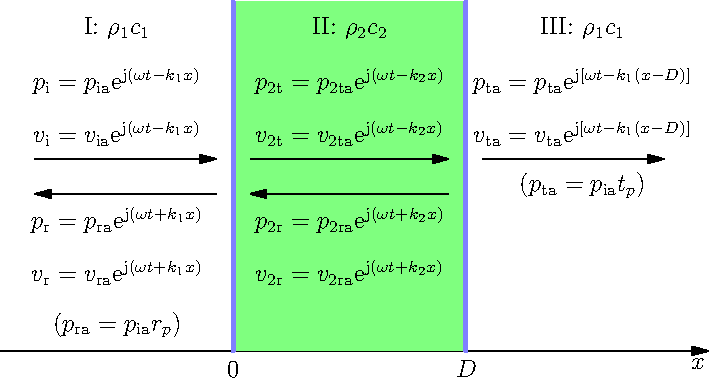
\includegraphics[width=0.8\textwidth]{img/idealfluid/planeVertIncPartition.pdf}
	\end{figure}
	$$
	v\st{ia} = \frac{p\st{ia}}{z_1}\qc
	v\st{ra}=-r_pv\st{ia}\qc
	v\st{2ta} = \frac{p\st{2ta}}{z_2}\qc
	v\st{2ra} = -\frac{p\st{2ra}}{z_2}\qc
	v\st{ta} = \frac{p\st{ta}}{z_1} 
	=v\st{ia}t_p$$
\end{frame}

\begin{frame}{Transmission through a Partition}
	\begin{outline}
		\1 boundary conditions
		$$x = 0: \quad 
		\begin{cases}
			1+r_p &= A+B\\
			z_{12}(1-r_p) &= A-B	
		\end{cases}
		\qc
		x= D:\quad 
		\begin{cases}
			A\me^{-\mj k_2 D} +B\me^{\mj k_2D}&=t_p\\
			A\me^{-\mj k_2 D} -B\me^{\mj k_2D}&=z_{12}t_p
		\end{cases}
		$$
		$$\qty(
		A = \frac{p\st{2ta}}{p\st{ia}}
		\qc 
		B = \frac{p\st{2ra}}{p\st{ia}}
		)
		$$
		\1 reflection and transmission coefficients
		$$ r_p = \frac{z\st{s}(x=0) - z_1}{z\st{s}(x=0)+z_1}
		= \frac{z_{12}-z_{21}}{z_{12}+z_{21} -2\mj \cot k_2 D}$$
		$$ t_p = \frac{-1}{\cos k_2 D + \mj \dfrac{z_{12}+z_{21}}{2}
	\sin k_2 D}$$
		\1 sound intensity
		$$t_I = \frac{I\st{t}}{I\st{i}} = |t_p|^2\qc r_I = \frac{I\st{r}}{I\st{i}}
		 = |r_p|^2\imp r_I+t_I = 1 $$
		$$t_I = \frac{1}{1+\dfrac{1}{4} (z_{12}-z_{21})^2 \sin^2 k_2 D}$$
	\end{outline}
\end{frame}

\begin{frame}{Partition: $t_I$}
	\begin{figure}
		\centering
		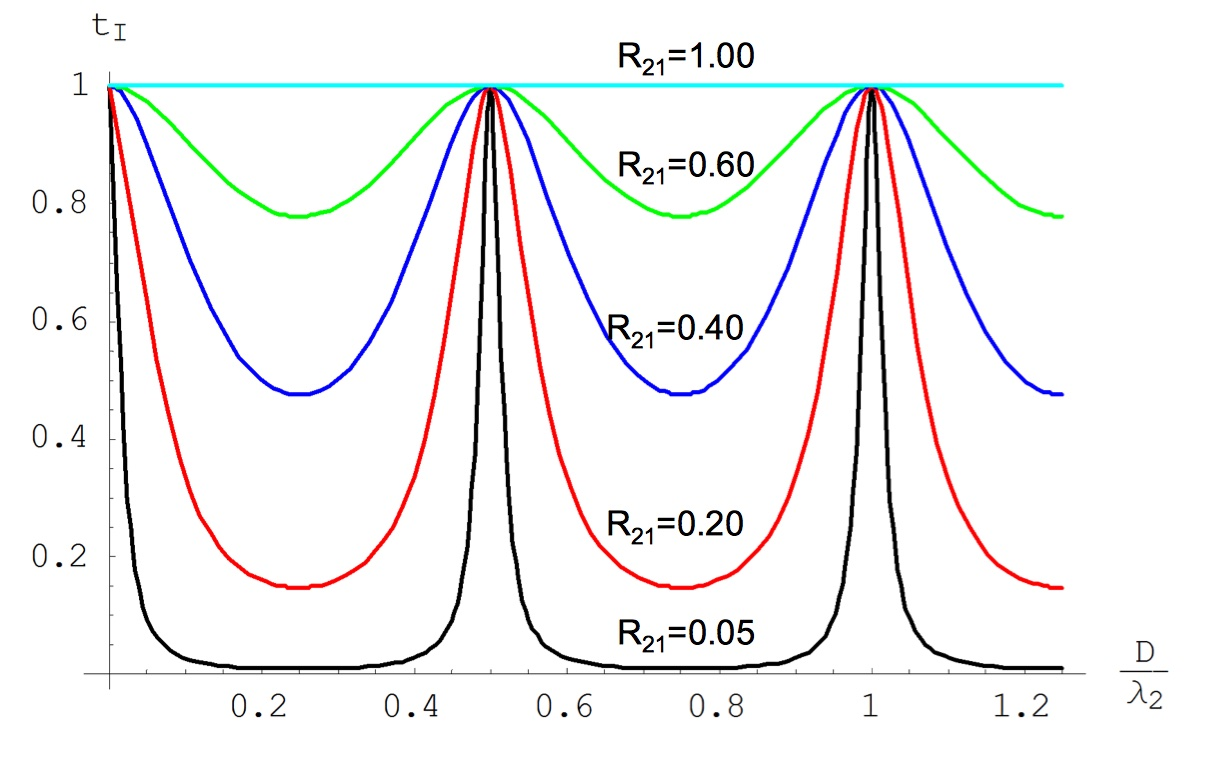
\includegraphics[width=0.9\textwidth]{img/idealfluid/planeVertIncPartitionTi.jpg}
	\end{figure}
\end{frame}

\begin{frame}{Thin Partition; Resonant Transmission; Insulation}
	\begin{outline}
		\1 thin partition
		$$k_2D\ll 1 \Leftrightarrow \lambda_2 \gg 2\uppi
		D\Leftrightarrow f\ll \frac{c_2}{2\uppi D}$$
		$$\imp t_I = 1-\frac14 (z_{12}-z_{21})^2 (k_2D)^2 +O(k_2D)^4\approx 1$$
		\1 resonant transmission at half wavelengths
		$$k_2D=n\uppi\qc D = n \frac{\lambda_2}{2} \qc (n=1,2,\cdots)
		\imp t_p = \frac{p\st{ta}}{p\st{ia}}=(-1)^n\qc t_I = 1$$
		\1 insulation at quater wavelengths
		$$k_2 D = (2n-1)\frac{\uppi}{2} \Leftrightarrow
		D=(2n-1)\frac{\lambda_2}{4}\qc (n=1,2,\cdots)$$
		$$\imp t_I = \frac{4}{(z_{12}+z_{21})^2}
		\xrightarrow{z_{12}\to \infty \qor z_{12} \to 0} 0$$
	\end{outline}
\end{frame}

\begin{frame}{Transfer Impedance Method}
	\begin{outline}
		\1 the specific acoustic impedance at $x$: $z\st{s} (x)$
		$$z\st{s}(x\to 0^-) = z_1 \frac{p\st{ia}+p\st{ra}}{p\st{ia}-p\st{ra}}
		\qc 
		z\st{s}(x\to 0^+) = z_2 \frac{p\st{2ta}+p\st{2ra}}{p\st{2ta}-p
		\st{2ra}}
		$$
		$$
		z\st{s}(x\to D^-) = z_2 \frac{p\st{2ta}\me^{-\mj k_2 D}+p\st{2ra}
		\me^{\mj k_2D}}{p\st{2ta}\me^{-\mj k_2D}-p\st{2ra}\me^{\mj k_2D}}
		\qc
		z\st{s}(x\to D^+) = z_1 
		$$
		\1 at surface $x=D$
		$$z\st{s}(x \to D^-) = z\st{s}(x \to D^+) \imp
		r_{p,D} \equiv \frac{p\st{2ra}\me^{\mj k_2D}}{p\st{2ta}\me^{
		-\mj k_2D}} = \frac{z\st{s}(x\to D^+) - z_2}{z\st{s}(x\to D^-)+z_2}
		$$
		$$\imp \frac{p\st{2ra}}{p\st{2ta}} = \me^{-2\mj k_2 D}
		\frac{z\st{s}(x\to D^+) - z_2}{z\st{s}(x\to D^-)+z_2}
		$$
		\1 the \emph{Transfer Impedance Formula}
		$$
		z\st{s} (x=0) = z_2 \frac{z\st{s}(x=D) +\mj z_2 \tan k_2 D}{
			z_2+\mj z\st{s}(x=D)\tan k_2D}
			$$
	\end{outline}
\end{frame}

\begin{frame}{Transmission through a Partition}
	\begin{outline}
		$$z\st{s}(x\to D^+) = z\st{s1} = z_1$$
		\1 according to the transfer impedance formula, we have 
		$$z\st{s}(x=0) = z_2 \frac{z_1+\mj z_2 \tan k_2D}{z_2 +\mj z_1 
		\tan k_2D}$$
		\1 reflection coefficient
		$$ r_p = \frac{z\st{s}(x=0) - z_1}{z\st{s}(x=0)+z_1}
		= \frac{z_{12}-z_{21}}{z_{12}+z_{21} -2\mj \cot k_2 D}$$
	\end{outline}
\end{frame}

\begin{frame}{Transmission Loss, TL}
	\begin{outline}
		\1 \emph{Transmission Loss} or \emph{Sound Redution}
		$$\mathrm{TL} = -10\lg t_I \qc (\si{dB})$$
		\1 a partition
		$$\mathrm{TL} = 10 \lg \qty[1+\dfrac14\qty(z_{12}-z_{21})^2 \sin^2 k_2D]
		$$
		\1 if (1) $z_{21}\ll 1 \Leftrightarrow z_1\ll z_2$ (\emph{Hard Wall}) 
		and (2) $k_2D<0.5$ (\emph{Low Frequency})
		$$ \mathrm{TL} \approx 10\lg \qty[1+\dfrac14 (z_{12}k_2D)^2] 
		= 10\lg \qty[1+\qty(\dfrac{\omega M_2}{2z_1})^2]
		\qc (M_2 = \rho_2 D)$$
		\1 if (3) $\omega M_2 \gg z_1$ (\emph{Heavy}) 
		$$ \mathrm{TL} \approx 20 \lg \qty(\dfrac{\omega M_2}{2z_1})$$
		\1 \emph{The Mass-Frequency Law}
		$$ \mathrm{TL} = -42 + 20\lg f + 20 \lg M_2 \qc (\si{dB})$$
		\1 conclusion: $D\to 2D$ or $f\to 2f$ $\imp \Delta \mathrm{TL} 
		=6 \mathrm{dB}$
	\end{outline}
\end{frame}

\begin{frame}{Transmission Through a Partition}
	\begin{outline}
		\1 a \emph{partition} is placed along $(0,D)$
	\end{outline}
	\begin{figure}
		\centering
		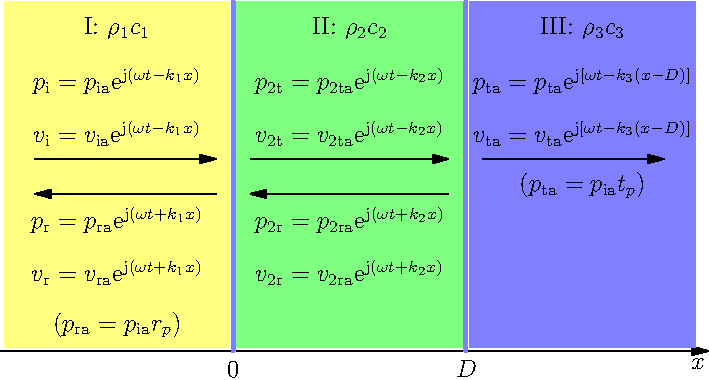
\includegraphics[width=0.8\textwidth]{img/idealfluid/planeVertIncPartition3.pdf}
	\end{figure}
	$$
	v\st{ia} = \frac{p\st{ia}}{z_1}\qc
	v\st{ra}=-r_pv\st{ia}\qc
	v\st{2ta} = \frac{p\st{2ta}}{z_2}\qc
	v\st{2ra} = -\frac{p\st{2ra}}{z_2}\qc
	v\st{ta} = \frac{p\st{ta}}{z_3} 
	=v\st{ia}t_p$$
\end{frame}


\begin{frame}{Partition}
	\begin{outline}
		\1 transfer impedance and sound pressure reflection coefficient
		$$
		z\st{s}(x\to 0^+) = z_2 \frac{z_3+\mj z_2\tan k_2D}{z_2+\mj z_3 \tan
		k_2 D}		\imp 
		r_p = \frac{z_2(z_3-z_1)+\mj (z_2^2-z_1 z_3)\tan k_2D}{z_2(z_3+z_1)
		+\mj (z_2^2+z_1z_3)\tan k_2D}
		$$
		\1 sound intensity transmission coefficients
		$$t_I = 1-|r_p|^2 = \frac{4z_1z_3}{(z_1+z_3)^2 \cos^2 k_2 D +(z_2+z_1z_3/z_2)^2
		\sin^2 k_2D}$$
		\1 when $k_2D=(1/2+n)\uppi$
		$$t_I = \frac{4x}{(1+x)^2}\qc \qty(x=z_{21}z_{23})$$
		$$\pdv{t_I}{x} = 0\imp x= 1\imp z_2 = \sqrt{z_1 z_3} \qc t_I(x=1) = 1$$
		\1 impedance matching (\emph{Anti-reflective coat})
		$$
		z\st{s}(x\to 0^+) = z_2 \frac{z_3+\mj z_2\tan k_2D}{z_2+\mj z_3 \tan
		k_2 D} \xrightarrow{k_2D=\uppi/2} \frac{z_2^2}{z_3} 
		\xleftrightarrow{\text{match}} z_1 \imp z_2 = \sqrt{z_1 z_3}$$
	\end{outline}
\end{frame}

\begin{frame}{An example}
	\begin{outline}
		\1 air: $z_1 = 415 \mathrm{Rayl}$; water: $z_3 = 1.48 \mathrm{M Rayl}$
		$$
		1 \si{Raly} = 1 \si{\Pa \cdot \s \cdot \m^{-1}}
		 = 1 \si{\kg\cdot \m^{-2} \cdot \s^{-1}} = 
		 1 \si{\N \cdot \s \cdot \m^{-3}}$$
		\1 Anti-reflective coat: $z_2$
	\end{outline}
	\begin{figure}
		\centering
		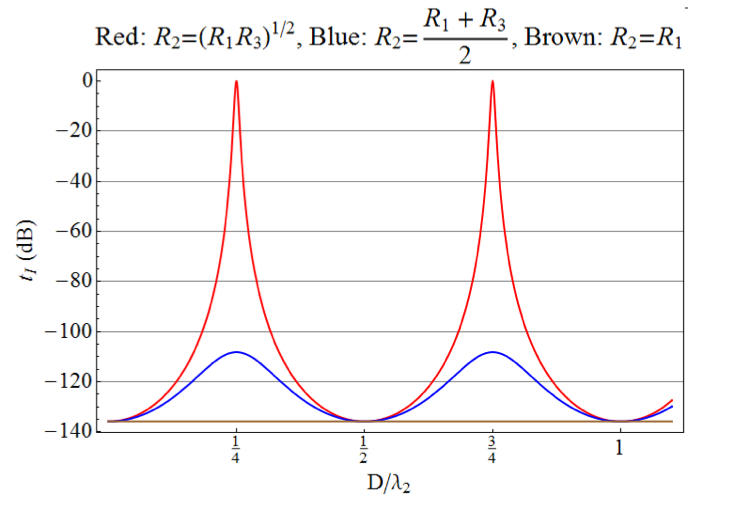
\includegraphics[width=0.8\textwidth]{img/idealfluid/PlaneVertIncARC.jpg}
	\end{figure}
\end{frame}


\subsection{Homework}
\begin{frame}{Homework}
	\begin{outline}[enumerate]
		\1 Textbook B: 4-18
		\1 Textbook B: 4-19
		\1 Textbook B: 4-21
		\1 Textbook B: 4-23
	\end{outline}
\end{frame}

\section{Standing Waves}
\begin{frame}{Standing Waves}
	\begin{outline}
		\1 animation: \url{www.walter-fendt.de/html5/phen/standingwavereflection_en.htm}
		\1 suppose 2 propagating waves in inverse directions
		$$p_\pm = A_\pm \me^{\mj (\omega t \mp kx )}$$
		\1 the resultant field
		$$ p\st{tot} = p_+ + p_- = 2A_- \cos kx \me^{mj \omega t}
		+(A_+ - A_- ) \me^{\mj (\omega t - kx)}$$
		\1 if $A_+=A_- \imp$ standing waves
		$$p\st{tot} = 2A_+ \cos kx \me^{mj \omega t}$$
		\1 node
		$$kx_m = \qty(m-\frac12)\uppi \qc x_m = \frac14(2m-1)\lambda\qc m\in \Z$$
		\1 antinode
		$$kx_n = n\uppi\qc x_n=\frac12 n\lambda\qc n\in \Z$$
	\end{outline}
\end{frame}

\begin{frame}{Standing Waves}
	\begin{outline}
		\1 sound field
		$$\begin{cases}
			p\st{tot} & = p\st{a} \cos kx\ \me^{\mj \omega t}\\
			v\st{tot} & = -\dfrac{1}{\mj k z_0}\displaystyle\pdv{p}{x} 
			= -\mj \frac{p\st{a}}{z_0}\sin
			kx\ \me^{\mj \omega t}
		\end{cases}
		$$
		\1 specific acoustic impedance
		$$z\st{s} = \frac{p\st{tot}}{v\st{tot}}
		=\mj z_0 \cot kx$$
		\1 time average of energy density
		$$\overline{\eps}\st{tot} = \frac12 \rho_0 \overline{v^2\st{tot}}
		+\frac12\beta_{\mathrm{s},0} \overline{p^2\st{tot}}
		=\frac14 \rho_0 p\st{a}^2 \dfrac{\sin^2 kx}{z_0^2} +
		\frac14 \beta_{\mathrm{s},0} p\st{a}^2 \cos^2 kx = \frac14
		\beta\st{s,0} p\st{a}^2$$
		\1 sound intensity
		$$I = \frac12 \Re(p^*\st{tot} v\st{tot}) = \frac12 \Re\qty[p\st{a}^*
		\cos kx \qty(-\mj p\frac{\st{a}}{z_0} \sin kx)]=0$$

	\end{outline}
\end{frame}

\begin{frame}{Sound Interference}
	\begin{outline}
		\1 two waves ($n = 1,2$): same \emph{frequency} and fixed \emph{phase difference}
		$$p_n = p_{\mathrm{a},n} \me^{\mj \omega t} = 
		|p_{\mathrm{a},n} | \me^{\mj (\omega t-\phi_n)}\qc
		(\Delta \phi = \phi_2 - \phi_1 = \mathrm{const.})$$
		\1 According to the superposition theory, the \emph{total field} is
		$$p = \sum_{n=1}^2 p_n = p\st{a} \me^{\mj \omega t} = |p\st{a}|
		\me^{\mj(\omega t-\phi)}$$
		$$p\st{a} = \sum_{n=1}^2 p_{\mathrm{a},n}$$
		$$|p\st{a}| \me^{-\mj \phi} = \sum_{n=1}^2 |p_{\mathrm{a,}n}| \me^{
		-\mj \phi_n}$$
		$$
		\begin{cases}
			|p\st{a}|^2 & = |p\st{a1}|^2 + |p\st{a2}|^2 + 2
			|p\st{a1}||p\st{a2}| \cos \Delta \phi \\
			\tan \phi & = \dfrac{ |p\st{a1}|\sin \phi_1 + |p\st{a2}|\sin \phi_2
		}{|p\st{a}|\cos\phi_1 + |p\st{a2}|\cos\phi_2}
		\end{cases}
		$$
	\end{outline}
\end{frame}

\begin{frame}{Constructive and Destructive Interference}
	\begin{outline}
		\1 if the total field is propagating
		$$\overline{\eps} = \frac12 \beta{s,0} |p\st{a}|^2 =
		\overline{\eps_1} + \overline{\eps_2} + \beta_{s,0}
		|p\st{a1}||p\st{a2}| \cos\Delta \phi \qc \qty(\overline{
		\eps_n} = \frac12 \beta_{s,0} |p_{\mathrm{a},n}|^2)
		$$
		\1 enhancement
		$$
		\Delta \phi = 2m\uppi \qc(m \in \Z) \imp
		\begin{cases}
			|p\st{a}| & = |p\st{a1}| + |p\st{a2}|\\
			\overline{\eps} & = \overline{\eps_1}+\overline{\eps_2}
			+\beta_{s,0}|p\st{a1}||p\st{a2}|
		\end{cases}
		$$
		\1 cancellation
		$$
		\Delta \phi = (2m-1)\uppi \qc(m \in \Z) \imp
		\begin{cases}
			|p\st{a}| & = |p\st{a1}| - |p\st{a2}|\\
			\overline{\eps} & = \overline{\eps_1}-\overline{\eps_2}
			+\beta_{s,0}|p\st{a1}||p\st{a2}|
		\end{cases}
		$$
	\end{outline}
\end{frame}

\begin{frame}{Incoherent Waves}
	\begin{outline}
		\1 if $\omega_1 \neq \omega_2$
		$$p_n = |p_{\mathrm{a},n}| \me^{\mj(\omega_n t - \phi_n)}
	\qc (n=1,2, \omega_1\neq \omega_2)$$
		\1 the total field
		$$ p = \sum_{n=1}^2 |p_{\mathrm{a},n} | \me^{\mj (\omega_n t-\phi_n)}
		=|p\st{a}|\me^{\mj \phi}$$
		\begin{align*}
		|p\st{a}|^2 &= \qty[\Re(p_1+p_2)]^2 + \qty[\Im (p_1+p_2)]^2\\
		& = |p\st{a1}|^2 +|p\st{a2}|^2 +2|p\st{a1}||p\st{a2}| \cos\qty[
		(\omega_1-\omega_2) t+\Delta \phi]
		\end{align*}
		\1 as long as the eplapsed time is long enough
		$$\overline{|p\st{a}|^2} = |p\st{a1}|^2+ |p\st{a2}|^2$$
		$$\imp \overline{\eps} = \overline{\eps_1} + \overline{\eps_2}$$
	\end{outline}
\end{frame}

\subsection{Homework}
\begin{frame}{Homework}
	\begin{outline}[enumerate]
		\1 Textbook B: 4-25
		\1 Textbook B: 4-26
		\1 Textbook B: 4-28
		\1 Textbook B: 4-29
	\end{outline}
\end{frame}


\setcounter{framenumber}{0}
%%%%%%%%%%%%%%%%%%%%%%%%%%%%%%%%%%%%%%%%%%%%%%%%%%%%%%%%%%%%%%%%%%%%%%%%%%%%%%%%%%%%%%%%
\renewcommand{\titlestring}{Sound Waves in Ducts Filled with Fluids}
\title{\titlestring}
\part{\titlestring}
\lecture{\titlestring}{duct}
%%%%%%%%%%%%%%%%%%%%%%%%%%%%%%%%%%%%%%%%%%%%%%%%%%%%%%%%%%%%%%%%%%%%%%%%%%%%%%%%%%%%%%%%

\section{Plane Waves}
\begin{frame}{Plane Waves in Ducts}
	\begin{figure}
		\centering
		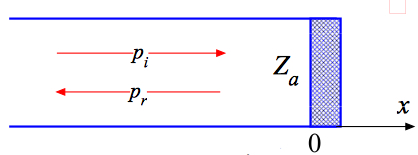
\includegraphics[width=0.5\textwidth]{img/duct/planeWavesInDucts.jpg}
	\end{figure}
	\begin{outline}
		\1 sound field
		$$\begin{cases}
			p\st{i} = p\st{ia} \me^{\mj(\omega t-kx)} \\
			p\st{r} = p\st{ra} \me^{\mj(\omega t+kx)}
		\end{cases}\qc
		\qty(p\st{ra} = r_p p\st{ia}\qc r_p = |r_p| \me^{\mj \sigma \uppi})
		$$
		\1 total field
		$$
			p(x,t) = p\st{i} + p\st{r} = p\st{a}(x) \me^{\mj \omega t}
		$$
		$$
		p\st{a}(x) = p\st{ia}\qty[\me^{-\mj kx} + |r_p|\me^{\mj (kx+\sigma \uppi)}
		] = |p\st{a}(x)| \me^{\mj \phi(x)}$$
		$$
		|p\st{a}(x)| = |p\st{ia}|\sqrt{1+|r_p|^2 +2|r_p|\cos \qty[2k\qty(
		x+\sigma \dfrac{\lambda}{4})]}
		$$
	\end{outline}
\end{frame}

\begin{frame}{Standing Waves Ratio}
	\begin{outline}
		\1 $p\st{max} = \max{|p\st{a}(x)|}$
		$$x = \pm n\frac{\lambda}{2} - \sigma \frac{\lambda}{4}\qc n\in \N$$
		\1 $p\st{min} = \min{|p\st{a}(x)|}$
		$$x = \pm (2n+1)\frac{\lambda}{2} - \sigma \frac{\lambda}{4}\qc n\in \N$$
		\1 \emph{SWR} (Standing Waves Ratio): (1) to obtain the \emph{amplitude}
		of reflection coefficient
		$$G\equiv \frac{|p\st{a}|\st{max}}{|p\st{a}|\st{min}} =
		\frac{1+|r_p|}{1-|r_p|} \Leftrightarrow 
		|r_p| = \frac{G-1}{G+1}$$
		\1 (2) to obtain the \emph{phase} of reflection coefficient
		$$
		(-x\st{min}) = \frac{\lambda}{4}\qty[(2n+1)+\sigma]\qc n \in \N
		$$
		$$
		(-x\st{min})\st{first} = (1+\sigma)\frac{\lambda}{4}$$
	\end{outline}
\end{frame}

\begin{frame}{Impedance in Ducts}
	\begin{figure}
		\centering
		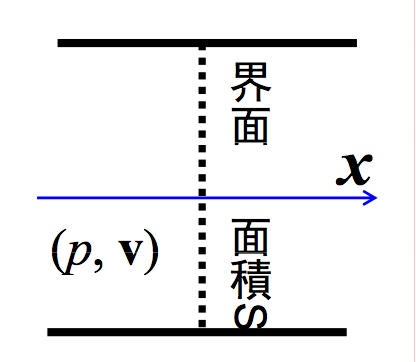
\includegraphics[width=0.25\textwidth]{img/duct/acousticImpedanceInDucts.jpg}
	\end{figure}
	\begin{outline}
		\1 cross section is $S$
		\1 the \emph{spatial} average pressure and volumetric flow rate
		$$\overline{p} = \frac1S \iint_S p\dd{S}
		\qc U = \iint_S \vb{v}\cdot \dd{\vb{S}}$$
		\1 the acoustic impedance of the cross section is defined as
		$$Z\st{a} \equiv \frac{\overline{p}}{U} = R\st{a} +\mj X\st{a}$$
		\1 the acoustic impedance is continuous in the both sides of the 
		cross section
		\1 for plane waves: $\vb{v} = v\vb{n}$
		$$\overline{p} = p\qc U = vS\qc Z\st{a} = \frac{z\st{s}}{S}
		\qc \qty(z\st{s}=\frac{p}{v})$$
	\end{outline}
\end{frame}

\begin{frame}{Reflection Coefficient in Ducts}
	\begin{figure}
		\centering
		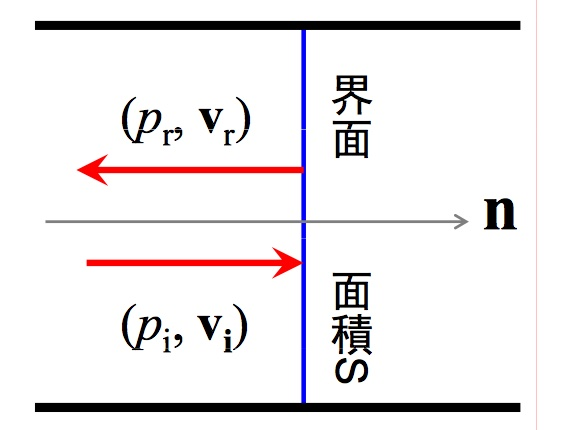
\includegraphics[width=0.25\textwidth]{img/duct/reflectionCoefInDucts.jpg}
	\end{figure}
	\begin{outline}
		\1 acoustic impedance of incident and reflective waves
		$$
		Z\st{ai} = \frac{p\st{i}}{Sv\st{i}} = \frac{z\st{si}}{S} = Z_0
		$$
		$$
		Z\st{ar} = \frac{p\st{r}}{Sv\st{r}} = \frac{z\st{sr}}{S} = -Z_0
		$$
		$$
		\qty(Z_0 = \frac{\rho_0c_0}{S}=z_0)
		$$
		\1 total acoustic impedance and reflection coefficient
		$$
		Z\st{a} = \frac{p}{Sv} = \frac{p\st{i}+p\st{r}}{S(v\st{i}+v\st{r})}
		=Z_0 \frac{1+r_p}{1-r_p}
		\Leftrightarrow
		r_p = 
		\frac{Z\st{a}-Z_0}{Z\st{a}+Z_0}$$
	\end{outline}
\end{frame}

\begin{frame}{Specific Acoustic Impedance Ratio and Reflection Coefficient}
	\begin{outline}
		\1 specific acoustic impedance ratio of the load
		$$\zeta\st{s} = \frac{z\st{s}}{z_0} = x\st{s} +\mj y\st{s}\qc(z_0 = \rho_0
		c_0)$$
		\1 acoustic impedance ratio of the load
		$$\zeta\st{a} = \frac{Z\st{a}}{Z_0} = x\st{a} +\mj y\st{a}\qc
		\qty(Z_0 = \frac{z_0}{S})$$
		\1 plane waves: $\zeta\st{s}=\zeta\st{a}=\zeta$
		\1 reflection coefficient 
		$$r_p = |r_p| \me^{\mj \sigma \uppi} =
		\frac{\zeta\st{a}-1}{\zeta\st{a}+1} = \frac{x\st{a}-1+\mj y\st{a}}
		{x\st{a}+1+\mj y\st{a}}$$
		\1 sound intensity reflection coefficient
		$$r_I = |r_p|^2 = \frac{(x\st{a}-1)^2 +y\st{a}^2}{(x\st{a}+1)^2+y\st{a}^2}
		=\frac{(R\st{a}-Z_0)^2+X\st{a}^2}{(R\st{a}+Z_0)^2+X\st{a}^2}
		$$
		\1 sound absorption coefficient
		$$\alpha = 1-r_I = \frac{4x\st{a}}{(x\st{a}+1)^2+y\st{a}^2}
		=\frac{\alpha\st{r}}{1+\qty(\dfrac{y\st{a}}{1+x\st{a}})^2}
		\qc \alpha\st{r} = \alpha|_{y\st{a}=0} = \frac{4x\st{a}}{(1+x\st{a})^2}
		$$
	\end{outline}
\end{frame}

\begin{frame}{Impedance Equation}
	\begin{outline}
		\1 magnitude and phase of the reflection coefficient 
		$$|r_p|^2 = \frac{(x\st{a}-1)^2 +y\st{a}^2 }{(x\st{a}+1)^2+y\st{a}^2}
		\qc 
		\tan (\sigma\uppi) = \frac{2 y\st{a}}{x\st{a}^2+y\st{a}^2-1}
		$$
		\1 impedance equation
		$$
		\begin{cases}
			\displaystyle
			\qty(x\st{a}-\frac{1+|r_p|^2}{1-|r_p|^2})^2+y\st{a}^2
			&=\qty(\dfrac{2|r_p|}{1-|r_p|^2})^2\\
			x\st{a}^2 + (y\st{a}-\cot \sigma \uppi)^2 &= \dfrac{1}{\sin^2 \sigma
			\uppi}
		\end{cases}
		$$
	\end{outline}
\end{frame}

\begin{frame}{Impedance Diagram}
	\begin{figure}
		\centering
		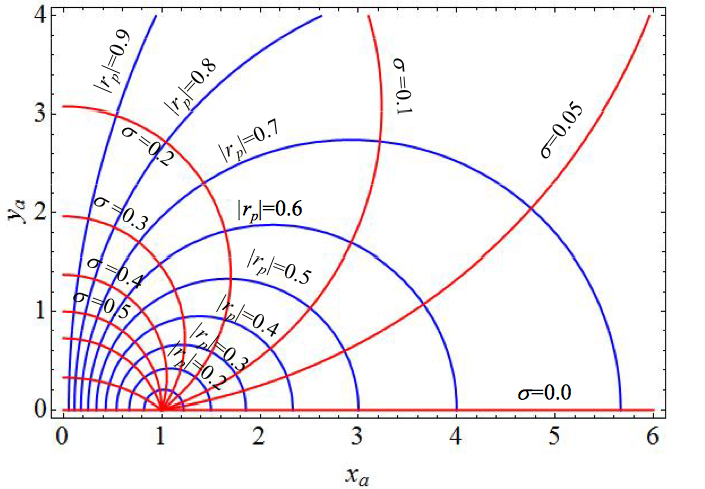
\includegraphics[width = 0.8\textwidth]{img/duct/impedanceDiagram.jpg}
	\end{figure}
\end{frame}

\section{Helmholtz Resonator}
\begin{frame}{Helmholtz Resonator}
	\begin{figure}
		\centering
		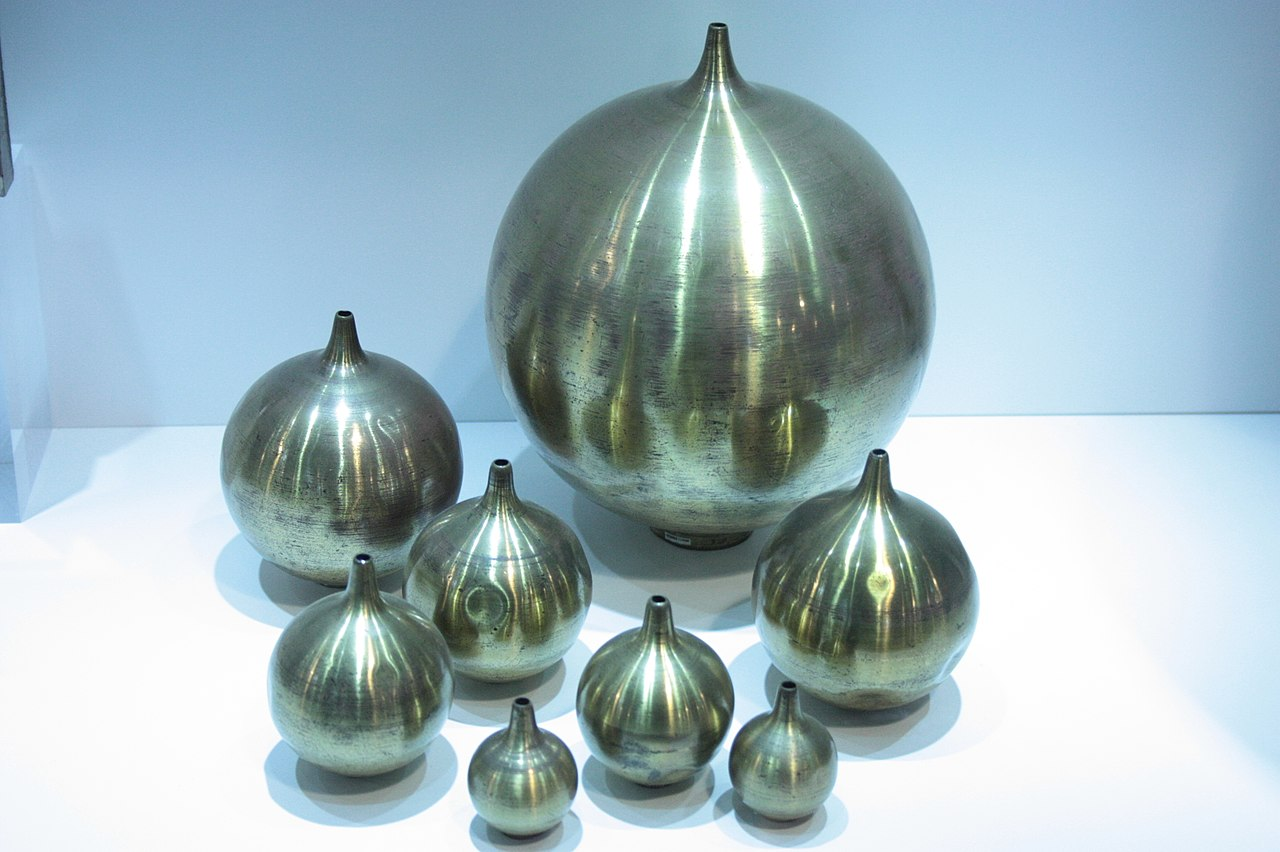
\includegraphics[width=0.8\textwidth]{img/duct/helmholtzResonatorArray.jpg}
	\end{figure}
\end{frame}

\begin{frame}{Helmholtz Resonator}
	\begin{figure}
		\centering
		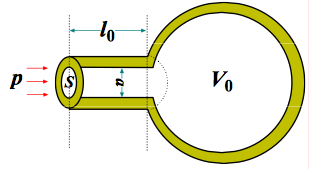
\includegraphics[width=0.3\textwidth]{img/duct/hemlholtzResonatorModel.jpg}
	\end{figure}
	\begin{outline}
		\1 \emph{short pipe}: cross section is $S$; radius is $a$; length is $l_0$
		\1 \emph{cavity}: volume is $V_0$; \emph{Assumption (1)}: boundary is very hard
		\1 \emph{fluid}: density is $\rho_0$; sound speed is $c_0$
		\1 \emph{Assumption (2)}: lumped system $\Leftrightarrow$
		$$
			\lambda \gg a, l_0, \sqrt[3]{V_0}
		$$
		\1 \emph{Assumption (3)}: big cavity $\Leftrightarrow$
		$$V_0\gg Sl_0$$
		\1 the short pipe moves like a piston $\imp$ mass is
		$$M\st{m} = \rho_0 Sl_0$$
		\1 considering the sound radiation effect at the orifice $\imp$
		the effective pipe length is
		$$l_0 \to l = l_0+\Delta l = l_0 +0.7a$$
		\1 the short pipe suffers friction from the wall $\imp$ mechanical
		resistance $R\st{m}$
	\end{outline}
\end{frame}

\begin{frame}{Helmholtz Resonator}
	\begin{outline}
		\1 the pressure changes as the air column in the short pipe moves
		$$p_1: P_0 \to P_0+p_1$$
		\1 adiabatic process: equation of state
		$$(P_0+p_1)(V_0-S\xi)^\gamma = P_0V_0^\gamma$$
		$$p_1 = \qty[\qty(1-\frac{S\xi}{V_0})^{-\gamma} -1]P_0
		\approx \gamma \frac{P_0S}{V_0}\xi 
		=\rho_0 c_0^2 \frac{S}{V_0}\xi = \kappa{s,0} \frac{S}{V_0}\xi
		$$
		\1 the force
		$$F = -p_1 S = -K\st{m} \xi\qc \qty(K\st{m} = \frac{1}{C\st{m}} = 
		\kappa_{s,0} \frac{S^2}{V_0})$$
	\end{outline}
\end{frame}

\begin{frame}{Dynamic Equation}
	\begin{outline}
		\1  dynamic equation for mechanics
		$$M\st{m}\dv{v}{t} +R\st{m} v + \frac{1}{C\st{m}}
		\int v\dd{t} = pS\qc(v=\dv{\xi}{t})$$
		\1 dynamic equation for acoustics
		$$M\st{a}\dv{U}{t} +R\st{a} U +\frac{1}{C\st{a}} \int U\dd{t}=p$$
		\1 provided that
			\2 volume velocity $U=vS$
			\2 acoustic mass $M\st{a}=M\st{m}/S^2$
			\2 acoustic resistance $R\st{a}=R\st{m}/S^2$
			\2 acoustic capacitance $C\st{a}=C\st{m}S^2$
	\end{outline}
\end{frame}

\begin{frame}{Resonance Sound Absroption Structure}
	\begin{outline}
		\1 acoustic mass $M\st{a} = \rho_0 l /S_0$, acoustic capacitance
		$C\st{a} =  \beta\st{s,0} V$, acoustic resistance $R\st{a}$
		\1 acoustic impedance ratio
		$$\zeta\st{a}=x\st{a}+\mj y\st{a} = \frac{Z\st{a}}{Z_0}$$
	\end{outline}
	\begin{figure}
		\centering
		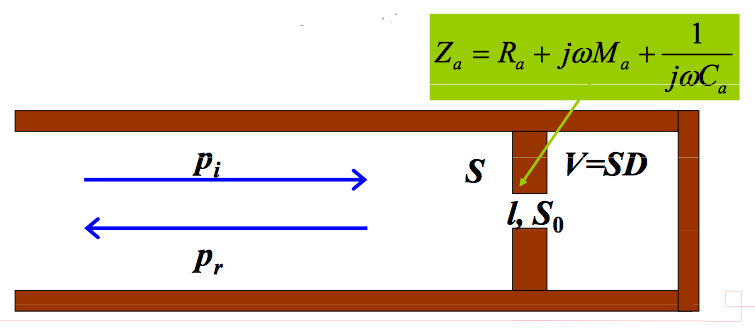
\includegraphics[width=0.8\textwidth]{img/duct/resonanceAbsorptionStructure.jpg}
	\end{figure}
\end{frame}

\begin{frame}{Resonance Sound Absorption Structure: Sound Absorption Coefficient}
	\begin{outline}
		\1 the correlation between SAC and frequency
		$$
		\alpha = \frac{\alpha\st{r}}{1+\qty(\dfrac{y\st{a}}{1+x\st{a}})^2}
		=\frac{\alpha\st{r}}{1+\qty[\dfrac{\omega M\st{a} - 1/(\omega C\st{a})}{
		R\st{a}'}]^2} = \frac{\alpha\st{r}}{1+Q\st{r}^2\qty(z-z^{-1})^2}
		$$
		$$
		\omega\st{r}\equiv \frac{1}{\sqrt{M\st{a}C\st{a}}}\qc
		\qty(z\equiv \frac{\omega}{\omega\st{r}}
		\qc 
		Q\st{r}\equiv \frac{\omega\st{r}M\st{a}}{R\st{a}'}
		\qc 
		R\st{a}'\equiv \frac{\rho_0c_0}{S}(1+x\st{a})
		=R\st{a} +\frac{\rho_0c_0}{S})
		$$
		\1 resonating conditions
		$$y\st{a}=0 \Leftrightarrow \omega M\st{a}-1/(\omega C\st{a}) = 0
		\Leftrightarrow \omega = \omega\st{r}\Leftrightarrow
		z=1$$
		\1 sound absorption coefficient
		$$\alpha\st{r} = \alpha|_{f=f\st{r}} = \frac{4x\st{a}}{(1+x\st{a})^2}
		=\frac{4\dfrac{\rho_0c_0}{S}R\st{a}}{\qty(\dfrac{\rho_0c_0}{S}+R\st{a})^2}
		$$
	\end{outline}
\end{frame}


\begin{frame}{Abrupt Interface}
	\begin{figure}
		\centering
		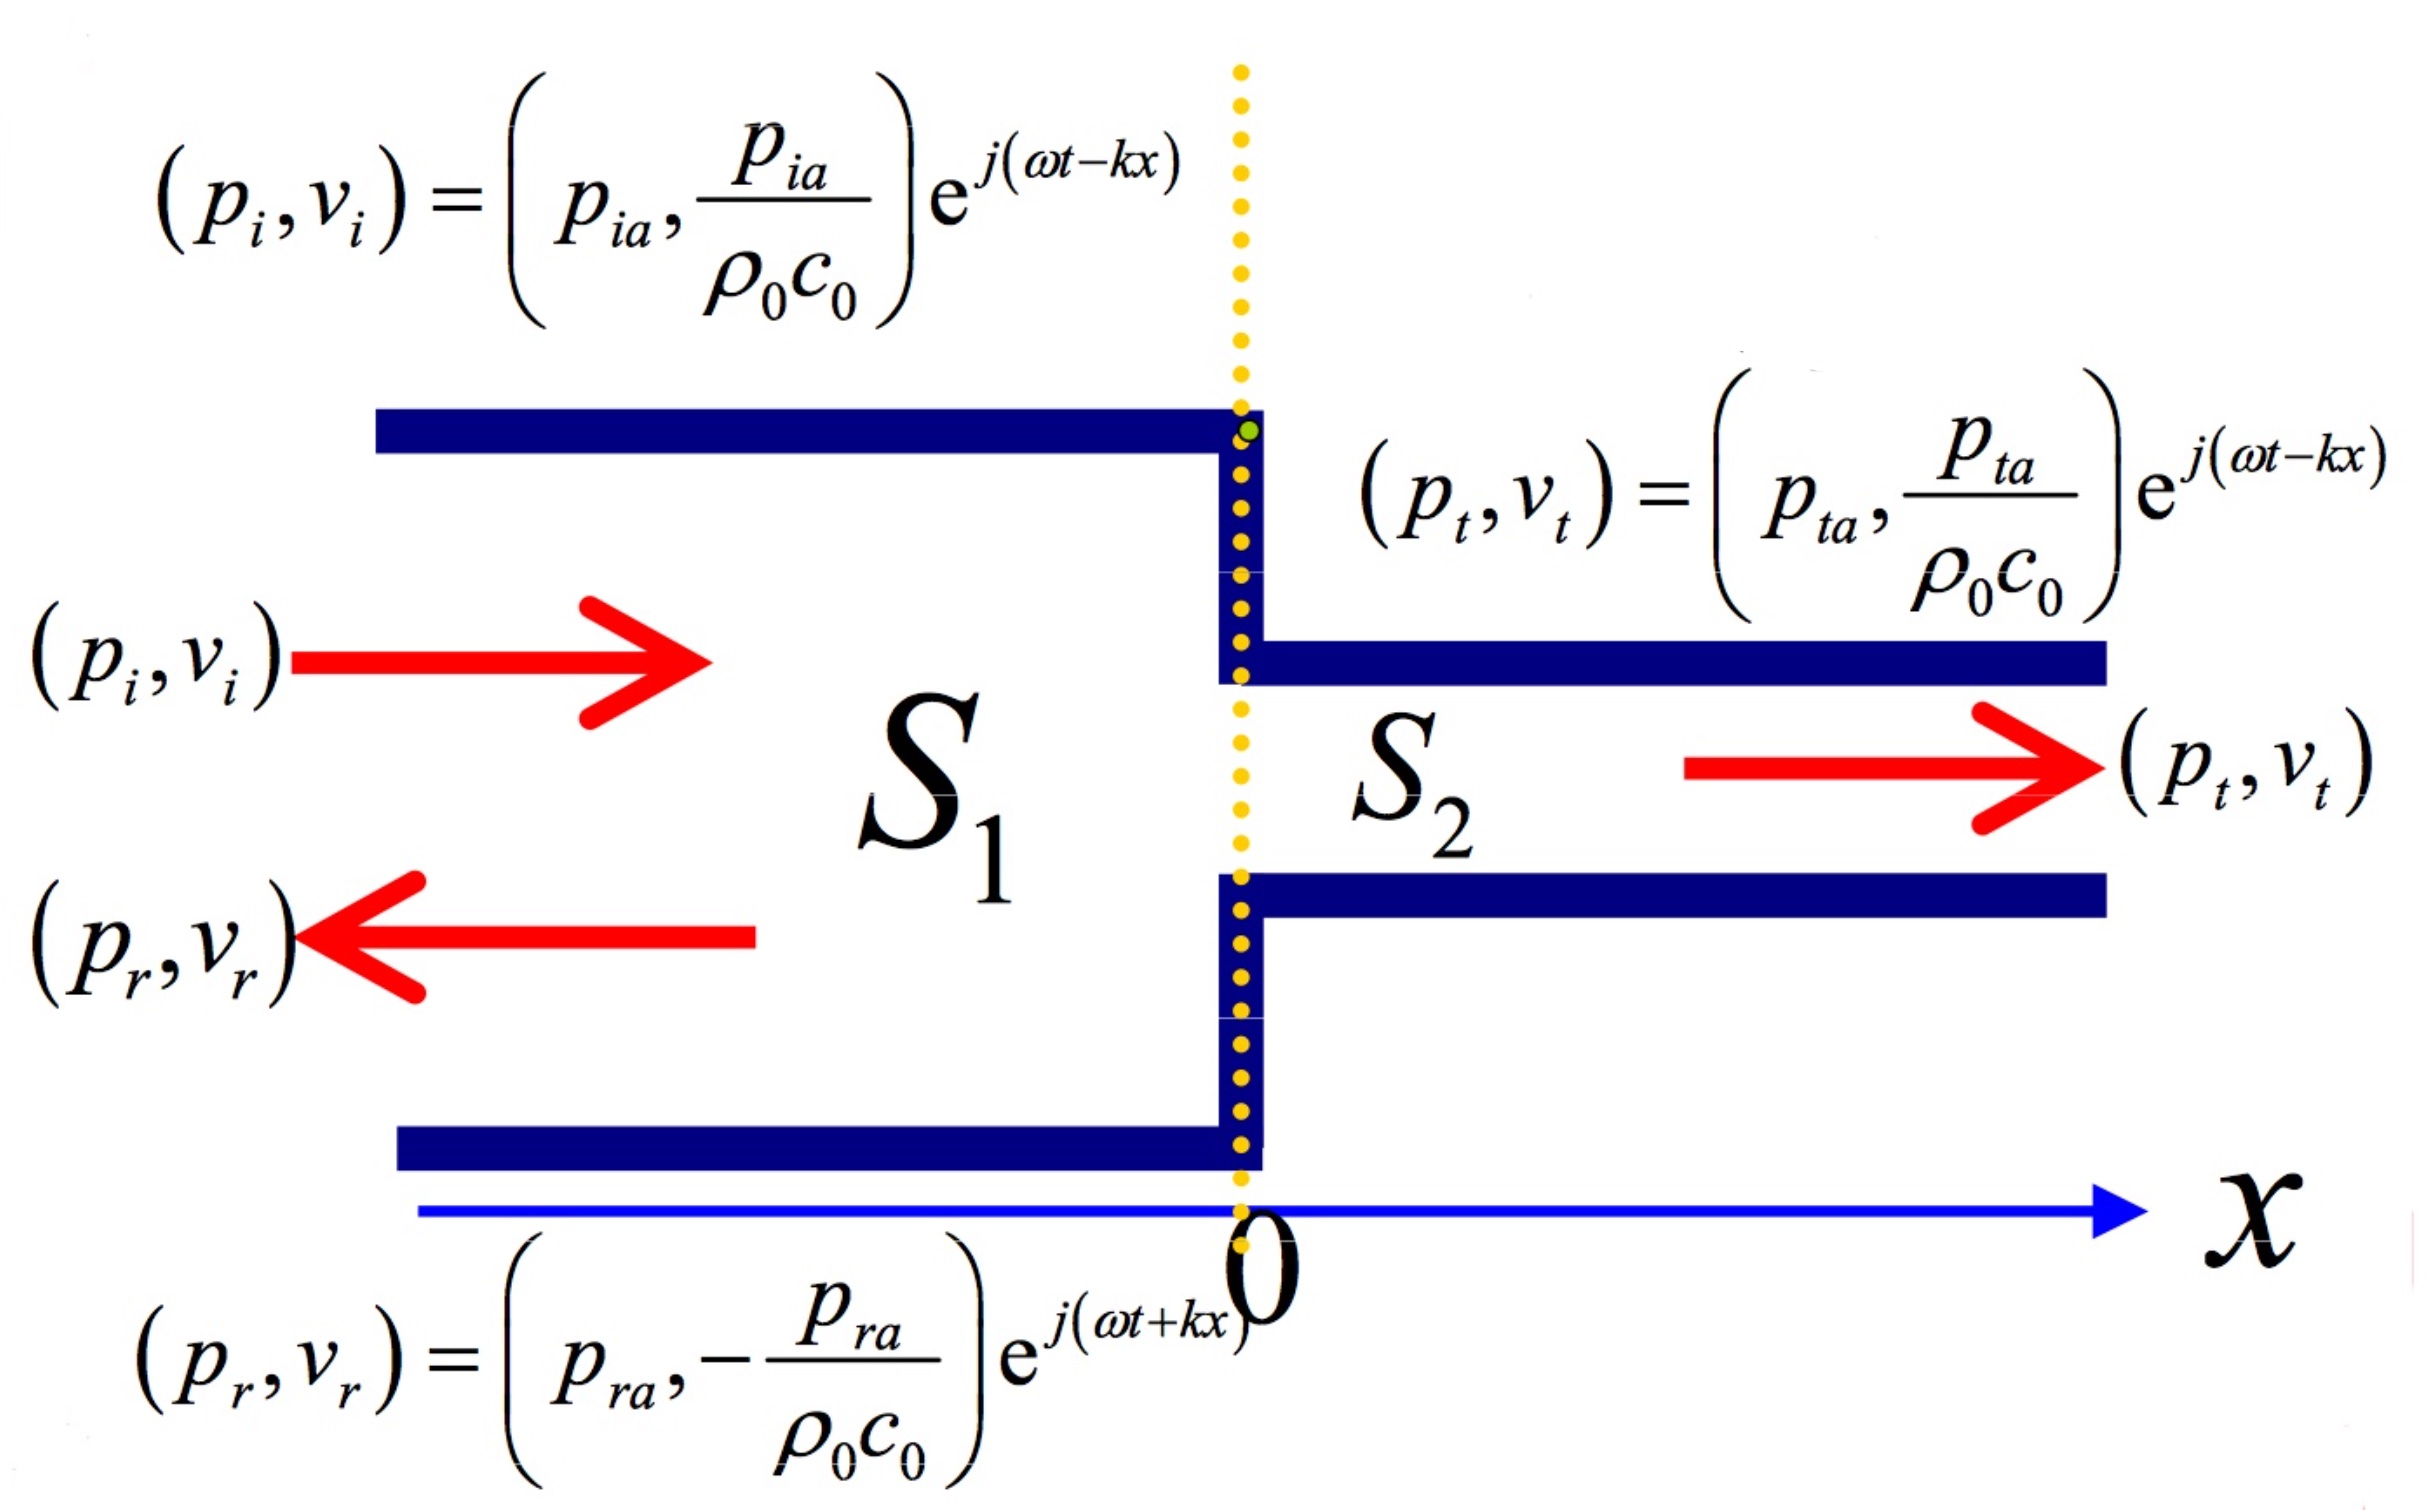
\includegraphics[width=0.8\textwidth]{img/duct/abruptInterface.jpg}
	\end{figure}
\end{frame}

\begin{frame}{Reflection and Transmission Coefficients}
	\begin{outline}
		\1 continuous quantity at $x=0$: pressure and \emph{volume flow rate (volume
		velocity)}
		$$\begin{cases}
			(p\st{i}+p\st{r})|_{x=0} &= p\st{t}|_{x=0}\\
			S_1 (v\st{i}+v\st{r})|_{x=0} &= S_2 v\st{t}|_{x=0}
		\end{cases}
		\imp
		\begin{cases}
			1+r_p&=t_p\\
			S_1(1-r_p)&=S_2t_p
		\end{cases}
		$$
		\1 reflection coefficient of pressure
		$$
		r_p \equiv \frac{p\st{ra}}{p\st{ia}} = 
		\frac{S_1-S_2}{S_1+S_2} =
		\frac{1/S_2-1/S_1}{1/S_2+1/S_1}=	
		\frac{Z\st{a2}-Z\st{a1}}{Z\st{a2}+Z\st{a1}}
		\qc \qty(Z_{\mathrm{a}i} = \frac{\rho_0c_0}{S_i}\qc i=1,2)
		$$
		\1 transmission coefficient of pressure
		$$
		t_p = 		\frac{2S_1}{S_1+S_2}=
		\frac{2/S_2}{1/S_2+1/S_1} = 
		\frac{2Z\st{a2}}{Z\st{a1}+Z\st{a2}}
		$$
		\1 reflection and transmission coefficients of intensity
		$$ r_I = \frac{I\st{r}}{I\st{i}} = \frac{|p\st{ra}|^2}{2\rho_0c_0}
		\Big/ \frac{|p\st{ia}|^2}{2\rho_0c_0} = |r_p|^2\qc
		 t_I = \frac{I\st{t}}{I\st{i}} = \frac{|p\st{ta}|^2}{2\rho_0c_0}
		\Big/ \frac{|p\st{ia}|^2}{2\rho_0c_0} = |t_p|^2$$
		\1 reflection and transmission coefficients of power
		$$r_W = \frac{I\st{r}S_1}{I\st{i}S_1} = r_I
		\qc t_W = \frac{I\st{t}S_2}{I\st{i}S_1} = \frac{4S_1S_2}{S_1+S_2}
		\qc r_W+t_W=1$$
	\end{outline}
\end{frame}


\begin{frame}{Acoustic Impedance Method}
	\begin{outline}
		\1 Acoustic impedance: $Z\st{a}(x)\equiv \dfrac{\overline{p}(x)}{U(x)}
		= \dfrac{p(x)}{v(x)S(x)}$
		$$
			Z\st{a}(x\to 0^-) = \left. \frac{p\st{i}+p\st{r}}{S_1(v\st{i}
			+v\st{r})} \right|_{x=0}
			=
			Z\st{a1} \frac{1+r_p}{1-r_p} 
			\qc \qty(
			Z\st{a1} = \frac{\rho_0c_0}{S_1})
		$$
		$$
		Z\st{a}(x\to 0^+) = \left.
		\frac{p\st{t}}{S_2v\st{t}}\right|_{x=0}
		=
		Z\st{a2}\qc \qty(Z\st{a2}=\frac{\rho_0c_0}{S_2})$$
		\1 continous conditions
		$$Z\st{a}(x\to 0^-) = Z\st{a}(x\to 0^+)$$
		$$\imp Z\st{a1} \frac{1+r_p}{1-r_p} = Z\st{a2}$$
		\1 reflection coefficient
		$$
		\imp r_p = \frac{Z\st{a2}-Z\st{a1}}{Z\st{a2}-Z\st{a1}}
		\imp r_p = \frac{1/S_2-1/S_1}{1/S_2+1/S_1} = \frac{S_1-S_2}{
		S_1+S_2}
		$$
	\end{outline}
\end{frame}

\section{Perforated Pipes}

\begin{frame}{Perforated Pipe}
	\begin{figure}
		\centering
		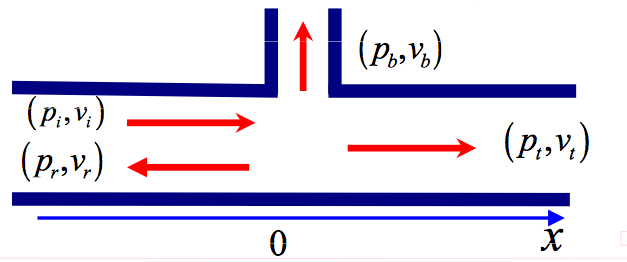
\includegraphics[width=0.7\textwidth]{img/duct/perforatedPipeMod.jpg}
	\end{figure}
	\begin{outline}
		\1 \emph{Assumption}: the size of the perforated pipe is much smaller 
		than the wavelength
		\1 acoustic impedance
		$$Z\st{b} = \frac{p\st{b}}{S\st{b}v\st{b}} = R\st{b}+\mj X\st{b}$$
		\1 boundary conditions at $x=0$
		$$
		\begin{cases}
			p\st{i}+p\st{r} = p\st{t} = p\st{b}\\
			U\st{i}+U\st{r} = U\st{t} + U\st{b}
		\end{cases}
		\qc 
		\qty(U\st{b} = \frac{p\st{b}}{Z\st{b}})
		$$
	\end{outline}
\end{frame}

\begin{frame}{Perforated Pipe}
	\begin{outline}
		\1 reflection and transmission coefficients of sound pressure
		$$ r_p = \frac{p\st{ra}}{p\st{ia}} = -\frac{Z\st{a0}/2}{Z\st{b}+
			Z\st{a0}/2}
			\qc 
			t_p = \frac{p\st{ta}}{p\st{ia}} = \frac{Z\st{b}}{Z\st{b}+
			Z\st{a0}/2}
			\qc 
			\qty(Z\st{a0}= \frac{\rho_0c_0}{S})
		$$
		\1 transmission coefficient of sound intensity
		$$t_I = |t_p|^2 = \frac{|Z\st{b}|^2}{|Z\st{b}+Z\st{a0}/2|^2}$$
		\1 acoustic impedance method
		$$Z\st{a}(x\to 0^-) = Z\st{a0} \frac{1+r_p}{1-r_p}$$
		$$Z\st{a}(x\to 0^+) = Z\st{a0} \parabins Z\st{b}
		=\frac{1}{1/Z\st{a0}+1/Z\st{b}}$$
		\1 reflection and transmission coefficients
		$$
		r_p = \frac{Z\st{a0}\parabins Z\st{b}-Z\st{a0}}{Z\st{a0}\parabins
		Z\st{b} + Z\st{a0}} = -\frac{Z\st{a0}/2}{Z\st{b}+Z\st{a0}/2}
		\qc
		t_p = 1+r_p = \frac{Z\st{b}}{Z\st{b}+Z\st{a0}/2}$$
	\end{outline}
\end{frame}

\begin{frame}{Perforated Helmholtz Resonator}
	\begin{figure}
		\centering
		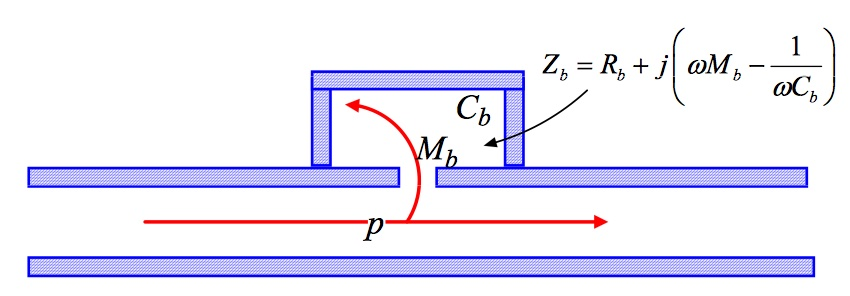
\includegraphics[width=0.6\textwidth]{img/duct/perforatedHelmholtz.jpg}
	\end{figure}
	\begin{outline}
		\1 acoustic impedance of perforated Helmholtz resonator
		$$Z\st{b} = R\st{b} + \mj \qty(\omega M\st{b} - \frac{1}{\omega
			C\st{b}})\qc Z\st{a0} = R\st{a0} = \frac{\rho_0c_0}{S}$$
		\1 transmission coefficient of sound intensity
		$$
		t_I = \frac{R\st{b}^2 + \qty(\omega M\st{b} - \dfrac{1}{\omega C\st{b}})
	^2}{\qty(R\st{b}+R\st{a0}/2)^2+\qty(\omega M\st{b} - \dfrac{1}{\omega C\st{
	b}})^2}
	\xrightarrow{R\st{b}\to 0} \frac{1}{1+ \dfrac{\qty(R\st{a0}/2)^2}{\qty(
		\omega M\st{b} - \dfrac{1}{\omega C\st{b}})^2}}
		\xRightarrow{\omega = \omega\st{r}} t_I \approx 0
	$$
	\end{outline}
\end{frame}

\section{Acoustic Impedance Transfer Formula}
\begin{frame}{Acoustic Impedance Transfer Formula}
	\begin{figure}
		\centering
		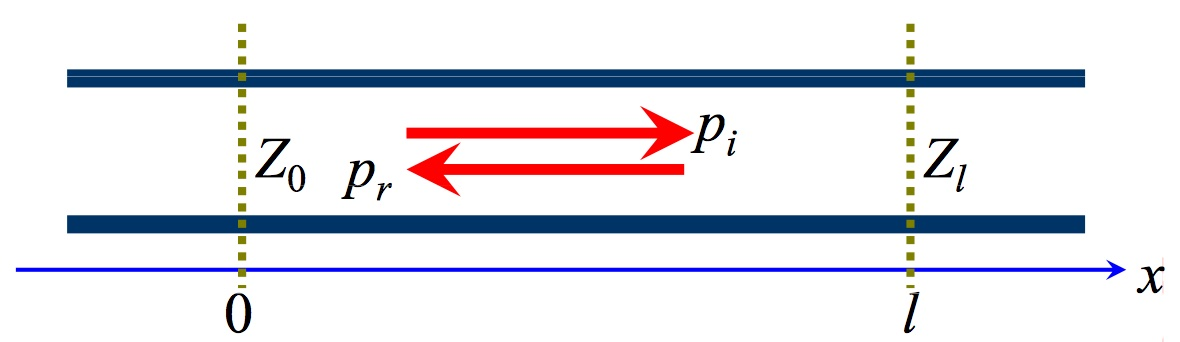
\includegraphics[width=0.8\textwidth]{img/duct/impedTrans.jpg}
	\end{figure}
	\begin{outline}
		\1 the acoustic impedance at $x=0$: $Z_0$; at $x=l$: $Z_l$
		\1 sound field inside the duct
		$$\begin{cases}
			p = p\st{i}+p\st{r}\\
			U = U\st{i} + U\st{r}
		\end{cases}
		$$
		$$\begin{cases}
			p\st{i} & = p\st{ia} \me^{\mj (\omega t-kx)}\qc 
			U\st{i}  = \dfrac{p\st{ia}}{R\st{a0}} \me^{\mj (\omega t-
			 kx)}\\
			p\st{r} & = p\st{ra} \me^{\mj (\omega t+kx)}\qc 
			U\st{r}  = -\dfrac{p\st{ra}}{R\st{a0}} \me^{\mj (\omega t+
			kx)}
		\end{cases}
		\qc \qty(R\st{a0}=\frac{\rho_0c_0}{S})$$
	\end{outline}
\end{frame}

\begin{frame}{Acoustic Impedance Transfer Formula}
	\begin{outline}
		\1 acoustic impedance at $x$
		$$
			Z\st{a}(x) = \frac{p(x)}{Sv(x)} 
			= R\st{a0}\frac{
			\me^{-\mj kx}+r_p \me^{\mj kx}}{\me^{-\mj kx}-r_p\me^{\mj kx}}
			= R\st{a0}\frac{
			1+r_p \me^{2\mj kx}}{1-r_p\me^{2\mj kx}}
		$$
		\1 when the $Z\st{a}(l) = Z_l$ is given $\imp$ reflection coeff. is 
		obtained
		$$ r_p \me^{2\mj kx} = \frac{Z\st{a}(l)-R\st{a0}}{Z\st{a}(l)+R\st{a0}}
		\imp
		Z\st{a}(x) = R\st{a0} \frac{Z\st{a}(l)-\mj R\st{a0}\tan k(x-l)}{
			R\st{a0}-\mj Z\st{a}(l)\tan k(x-l)}
		$$
		\1 specifically at $x=0$
		$$Z\st{a}(0) = R\st{a0}\frac{Z\st{a}(l)+\mj R\st{a0}\tan kl}{
			R\st{a0}+\mj Z\st{a}(l)\tan kl}$$
	\end{outline}
\end{frame}

\begin{frame}{Inserted Pipe}
	\begin{figure}
		\centering
		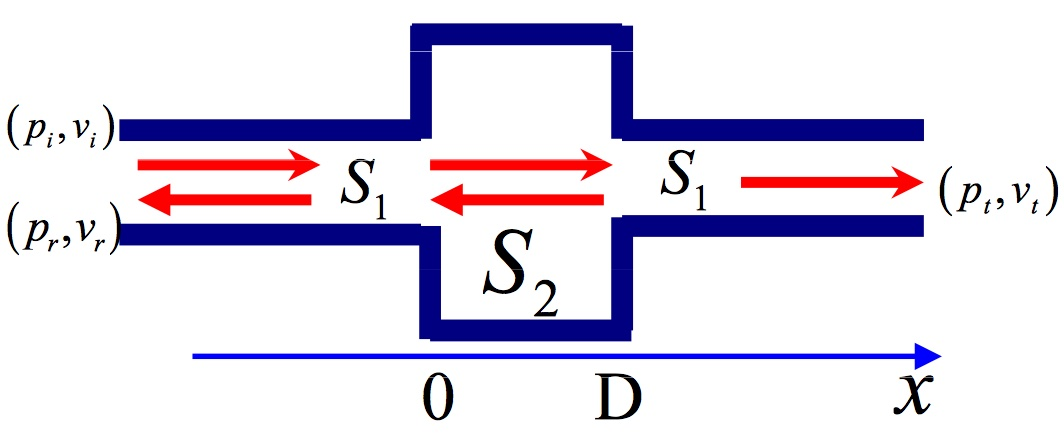
\includegraphics[width=0.7\textwidth]{img/duct/insertedPipe.jpg}
	\end{figure}
	\begin{outline}
		\1 review the transmission coefficient of sound intensity with a 
		inserted partition
		$$t_I = \frac{1}{1+\dfrac14 (z_{12}-z_{21})^2\sin^2 k_2D}$$
		\1 analogy: $z_{12}\leftrightarrow S_{21}$
		$$t_I = \frac{1}{1+\dfrac14 (S_{12}-S_{21})^2\sin^2 k_2D}$$
	\end{outline}
\end{frame}

\begin{frame}{$t_I$}
	\begin{figure}
		\centering
		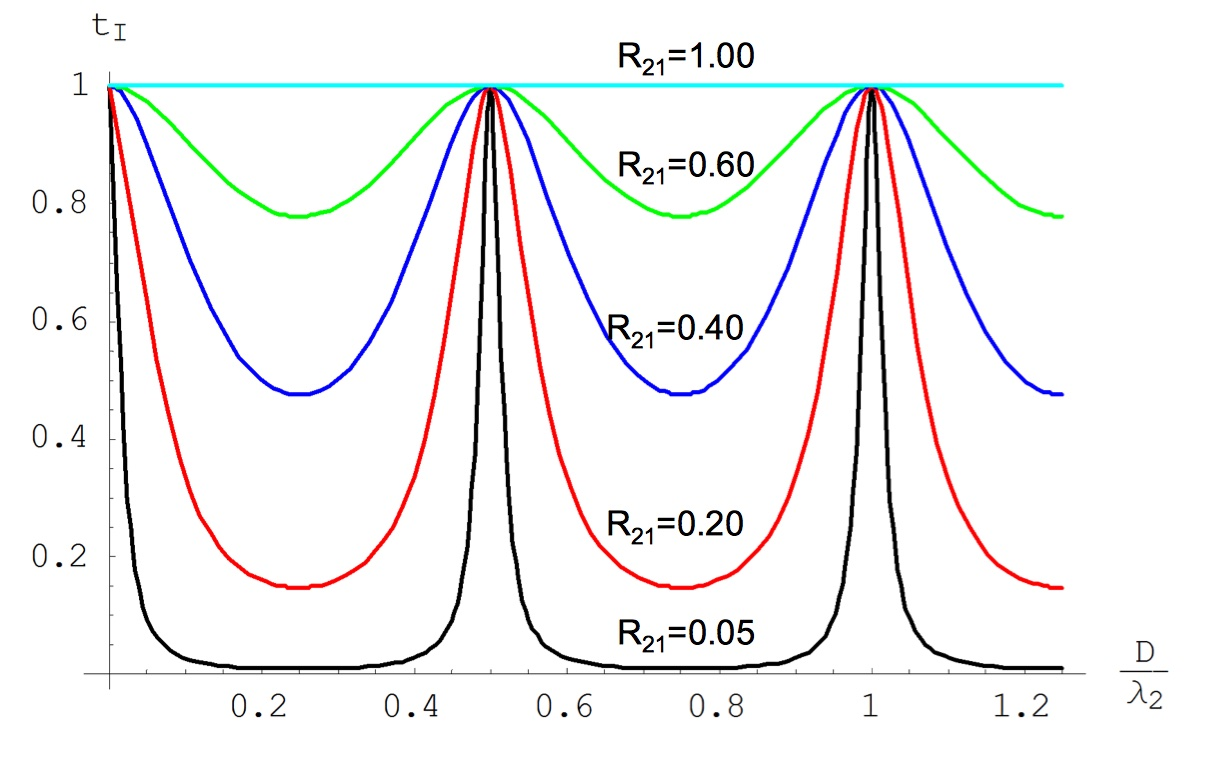
\includegraphics[width=0.9\textwidth]{img/idealfluid/planeVertIncPartitionTi.jpg}
	\end{figure}
\end{frame}

\begin{frame}{Sound Hard at End}
	\begin{outline}
		\1 sound hard at $x=l$ $\imp$ $v(l) =0$ $\imp$ $Z_l =\infty$
		$$
		Z\st{a}(0) = -\mj R\st{a0}\cot kl\qc \qty(R\st{a0}=\frac{\rho_0c_0}{
		S})$$
		\1 when $kl<1$
		\begin{align*}
			Z\st{a}(0) &= -\mj \frac{\rho_0c_0}{Skl} \qty[1-
			\frac13 (kl)^2+o((kl)^2)]\\
			&\approx -\mj \frac{\rho_0c_0}{Skl} \qty[1-\frac13
			(kl)^2]\qc (kl\ll 1)\\
			&= \frac{1}{\mj \omega C\st{a}}+\mj \omega\qty(\frac13 M\st{a})
			\qc \qty(C\st{a} = \beta_{s,0} V\qc M\st{a}=\frac{\rho_0 l}{S})
		\end{align*}
		\1 where
		$$
		\cot x = \frac1x - \frac{x}{3} + o(x)
		$$
	\end{outline}
\end{frame}

\begin{frame}{Open End}
	\begin{outline}
		\1 open end at $x=l$
		\1 assume (1): $ka<0.5$, where $a$ is the radius of
		the pipe
		$$Z\st{a}(l) \approx \mj X_{\mathrm{a}l}\qc
		\qty(X_{\mathrm{a}l} \approx \frac{8}{3\uppi} \frac{\rho_0c_0}{S}
		kz)$$
		\1 assume (2): $kl<0.5 \imp \tan kl \approx kl$
		\begin{align*}
		Z\st{a}(0) &\approx \frac{\rho_0c_0}{S} \frac{
			\mj X_{\mathrm{a}l}+\mj \dfrac{\rho_0c_0}{S} (kl)}{
				\dfrac{\rho_0c_0}{S}-X_{\mathrm{a}l} (kl)}\\
				&\approx \mj  \qty[X_{\mathrm{a}l} + \dfrac{\rho_0
				c_0}{S} (kl)]\\
				& = \mj \omega M\st{a} \qc \qty(
				M\st{a} = \frac{\rho_0(l+\Delta l)}{S}\qc
				\Delta l=\frac{8}{3\uppi}a \approx 0.85 a)
		\end{align*}
	\end{outline}
\end{frame}

\begin{frame}{Homework}
	\begin{outline}[enumerate]
		\1 Textbook B: 5-1
		\1 Textbook B: 5-3
		\1 Textbook B: 5-4
		\1 Textbook B: 5-7
		\1 Textbook B: 5-8
		\1 Textbook B: 5-9
		\1 Textbook B: 5-10
		\1 Textbook B: 5-13
		\1 Textbook B: 5-15
	\end{outline}
\end{frame}

\begin{frame}{Slowly Varying Pipe}
	\begin{figure}
		\centering
		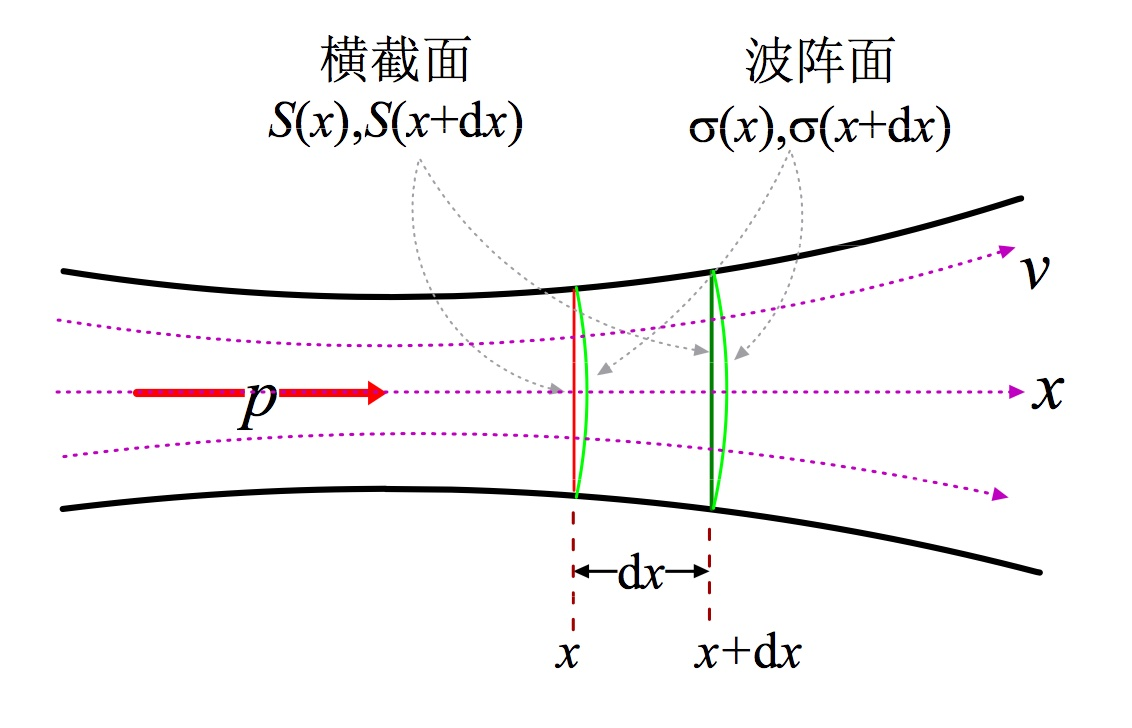
\includegraphics[width=0.8\textwidth]{img/duct/slowlyVaryingPipe.jpg}
	\end{figure}
\end{frame}
%%%%%%%%%%%%%%%%%%%%%%%%%%%%%%%%%%%%%%%%%%%%%%%%%%%%%%%%%%%%%%%%%%%%%%%%%%%%%%%%%%%%%%%%
\setcounter{framenumber}{0}
\renewcommand{\titlestring}{Radiation of Sound}

\part{\titlestring}
\title{\titlestring}
\lecture{\titlestring}{radiation}
%%%%%%%%%%%%%%%%%%%%%%%%%%%%%%%%%%%%%%%%%%%%%%%%%%%%%%%%%%%%%%%%%%%%%%%%%%%%%%%%%%%%%%%%

\begin{frame}{Pulsating Sphere}
	\begin{outline}
		\1 \emph{Pulsating Sphere}: acoustic radiation with spherical symmetry
		about a point
		\1 wave equations
		$$\frac{1}{r^2} \pdv{r}\qty(r^2 \pdv{p}{r}) - 
		\frac{1}{c_0^2}\pdv[2]{p}{t} = 0 \qor \qty[\pdv[2]{r} - \frac{1}{c_0^2}
	] (rp)=0 \qc (r>a)
		$$
			\2 $a$: the radius of the sphere
		$$p(r,t) = \frac{1}{r} f(r,t)$$
		\1 we have
		$$
		\imp \pdv[2]{f}{r} -\frac{1}{c_0^2} \pdv[2]{f}{t}=0
		$$
		\1 the general solution is 
		$$
		f(r,t) = A\me^{\mj(\omega t -kr)} + B\me^{\mj(\omega t+kr)}
		$$
		$$
		\imp p(r,t) = p\st{a} \me^{\mj (\omega t-kr)}
		\qc \qty(p\st{a} = \frac{A
		}{r})
		$$
		$$
		v_r(r,t)  = -\frac{1}{\mj k \rho_0 c_0} \pdv{p}{r}
		=v\st{a} \me^{\mj(\omega t-kr)} 
		\qc
		\qty[v\st{a} =\frac{p\st{a}}{\rho_0c_0}\qty(1+\frac{1}{\mj kr})]
		$$
	\end{outline}
\end{frame}

\begin{frame}{Pulsating Sphere}
	\begin{outline}
		\1 boundary conditions
		$$v_r(r,t)|_{r=a} = u(t) = u\st{a} \me^{\mj(\omega t-ka)}$$
		\1 we have
		$$A = \frac{\rho_0c_0a u\st{a}}{1+(\mj ka)^{-1}}
		=\frac{\mj k}{4\uppi} \frac{\rho_0c_0Q\st{a}}{1+\mj ka}
		\qc \qty(Q\st{a} \equiv 4\uppi a^2 u\st{a})
		$$
		\1 represent sound pressure, velocity and velocity potential with
		\emph{volume velocity} $Q(t)$
		$$
			\begin{cases}
				p& = \mj k \rho_0 c_0 \dfrac{Q(t)}{1+\mj ka} g(r) \\[0.5em]
				v_r & = - \dfrac{Q(t)}{1+\mj ka} g'(r) = 
				\dfrac{p}{\rho_0c_0} \qty(1+\dfrac{1}{\mj kr})
				= \mj k \dfrac{Q(t)}{1+\mj ka}g(r) \qty(1+\dfrac{1}{
				\mj kr})\\[0.5em]
				\Phi & = \dfrac{1}{\mj k \rho_0c_0} =
				\dfrac{Q(t)}{1+\mj ka} g(r)
			\end{cases}
		$$
		$$\qty(Q(t)\equiv Q\st{a}\me^{\mj \omega t}\qc
		g(r)\equiv \frac{\me^{-\mj kr}}{4\uppi r}
		=-\frac{\mj k}{4\uppi} h_0^{(2)}(kr)\qc
		h_0^{(2)}(z) = \frac{\me^{-\mj z}}{-\mj z})
		$$
	\end{outline}
\end{frame}

\begin{frame}{Small Sphere, Far-field, and Radiation Impedance}
	\begin{outline}
		\1 \emph{Assumption: Small Sphere}: $ka\ll 1$
		$$
		\imp \Phi \approx Q(t) g(r) \qc p \approx \mj k \rho_0 c_0 Q(t)g(r)
		$$
		\1 Far-field: $kr\gg 1$
		$$
			v_r \approx \frac{p}{\rho_0c_0}
		$$
			\2 like a plane wave!
		\1 radial specific acoustic impendace
		$$
		z\st{s} = \frac{p}{v_r} = \frac{\rho_0c_0}{1+(\mj kr)^{-1}}
		$$
		\1 radiation mechanical impedance 
		$$Z\st{r} = - \left. \frac{F\st{a}}{u}\right|_{r=a} 
		=S_0 z\st{s}|_{r=a} = R\st{r} +\mj X\st{r}$$
		$$R\st{r} = \rho_0 c_0 S_0 \frac{(ka)^2}{1+(ka)^2}
		\qc 
		X\st{r} = \rho_0 c_0 S_0 \frac{ka}{1+(ka)^2} >0
		\qc (S_0 = 4\uppi a^2)
		$$
	\end{outline}
\end{frame}

\begin{frame}{Green Functions with Infinitely Large Rigid Boundary}
	$$
		G(\vb{r};\vb{r}_0) = g(|\vb{r}-\vb{r}_0|) + g(|\vb{r}-\vb{r}'_0|), \quad 
		\begin{cases}
			\vb{r}_0 = (x_0,y_0,z_0)\\
			\vb{r}'_0 = (x_0,y_0,-z_0)
		\end{cases}
	$$
\end{frame}

\begin{frame}{Radiation from a Baffled Circular Plane Piston}
	\begin{outline}
		\1 only the sound field on the surface $xOz$ is needed to compute for symmetry
		\1 location of the field point $P$: $\vb{r}=r(\sin\theta,0,\cos\theta)$
		\1 volume velocity of an element on the piston: $\dd{Q_0}$
		\1 location of a point on the piston $\dd{Q}_0$: $\vb{r}_0 = \rho(\cos\phi,\sin\phi,0)$
		\1 distance between $P$ and $\dd{Q}_0$: $h=|\vb{r}-\vb{r}_0|\approx r-\rho\sin\theta \cos\phi, (r\gg a)$
		$$\Phi(\vb{r}) = \iint_{S_\text{pis}} 2g(\vb{r};\vb{r}_0) u\st{a}
		(\vb{r}_0) \dd{S_0} \xlongequal{u\st{a} =\text{const}} u\st{a}\iint_{S_\text{pis}} \frac{\me^{-\mj kh}}{2\uppi h}\dd{S_0}$$
	\end{outline}

\end{frame}

\begin{frame}{Radiation from a Baffled Circular Plane Piston}
	\begin{exampleblock}{Sound Field at Far Field (Radiation from a Baffled Circular Plane Piston) }
		$$\Phi(\vb{r},t)\approx 2Q(t)g(r)D(\theta) $$
		\begin{flalign*}
			\text{where}&& Q(t) = Q\st{a}\me^{\mj \omega t},\quad  Q
			\st{a} = u\st{a}\qty( \uppi a^2),\quad g(r) \equiv
			\frac{\me^{-\mj kr}}{4\uppi r},\quad D(\theta) \equiv \frac{2\upJ_1(ka\sin\theta)}{ka\sin\theta}  & &
		\end{flalign*}
	\end{exampleblock}
\end{frame}

\begin{frame}{Radiation from a Baffled Circular Plane Piston}{Radiation Directivity (Pattern)}
	\begin{outline}
		\1 the property of Bessel functions: $\qty[\dfrac{2\upJ_1(x)}{x}]_{x=0} = 1$
	\end{outline}

\end{frame}

%%%%%%%%%%%%%%%%%%%%%%%%%%%%%%%%%%%%%%%%%%%%%%%%%%%%%%%%%%%%%%%%%%%%%%%%%%%%%%%%%%%%%%%%
\setcounter{framenumber}{0}
\renewcommand{\titlestring}{Viscous Absorption of Sound}
\part{\titlestring}
\title{\titlestring}
\lecture{\titlestring}{viscosity}
%%%%%%%%%%%%%%%%%%%%%%%%%%%%%%%%%%%%%%%%%%%%%%%%%%%%%%%%%%%%%%%%%%%%%%%%%%%%%%%%%%%%%%%%


\begin{frame}
	\begin{figure}
		\centering
		\animategraphics[loop,controls,width=0.5\linewidth]{20}{gif/viscosities-}{0}{65}
		\footnote{Available at: https://www.wikiwand.com/en/Viscosity}
	\end{figure}
\end{frame}

\begin{frame}
	\begin{defi}[Viscosity]
		\begin{outline}
			\1 Definition 1. \emph{the first and second viscosity}
			$
				\mu_1, \mu_2
			$
			\1 Definition 2. \emph{the shear viscosity} $\eta$, and \emph{the bulk viscosity} $\zeta$
			\1 the relations:
			$$
				\begin{cases}
					\mu_1 = \eta\\
					\mu_2 = \zeta-\frac23 \eta
				\end{cases},
				\quad
				\begin{cases}
					\eta = \mu_1\\
					\zeta=\frac23 \mu_1+\mu_2
				\end{cases}
			$$
		\end{outline}
	\end{defi}
\end{frame}

\begin{frame}
	\begin{exampleblock}{Conservation of Momentum}
		\begin{outline}
		$$
			\dv{}{t}\iiint_V \rho v_i \dd{V} = \iiint_V \rho g_i \dd{V} - \oiint_S \rho v_i v_k \dd{S_k} + \oiint_S T_{ik} \dd{S_k}
		$$
		\1 \emph{Cartesian momentum density component}: $\rho v_i$
		\1 \emph{force density (force per volume)}: $\rho g_i$
		\1 \emph{stress tensor}: $T_{ik}$
		\end{outline}
	\end{exampleblock}

	\begin{outline}
		\1 by Gauss theorem: 
			$$\pdv{ }{t} \qty(\rho v_i) = \rho g_i - \pdv{}{x_k}\qty(\rho v_iv_k) + \pdv{}{x_k}\qty(T_{ik})$$
	\end{outline}

	\begin{alertblock}{Conservation of Momentum Equation}
		\begin{outline}
			\1 by using the Continuity Equation, we have 
			$$
			\rho \dv{v_i}{t} \equiv \rho \pdv{v_i}{t} +\rho v_{i,k} v_k = \rho g_i + \pdv{}{x_k}\qty(T_{ik})
			$$
		\end{outline}
	\end{alertblock}
\end{frame}

\begin{frame}
	\begin{block}{Strain and Stress}
		\begin{outline}
			\1 \emph{strain rate tensor} (\emph{deformation velocity tensor})
				$$
					d_{ij} \equiv \frac12(v_{i,j}+v_{j,i})
				$$
			\1 \emph{stress tensor}
			$$
				T_{ij} = \mu_1 \Theta \delta_{ij} + 2\mu_2 d_{ij}, \quad \qty(\Theta \equiv d_{kk}=\div \vb{v})
			$$
		\end{outline}
	\end{block}

\end{frame}

\begin{frame}{Navier-Stokes Equation}
	
	\begin{alertblock}{General Navier-Stokes Equation}
		$$
		\rho \dv{\vb{v}}{t} = \rho \vb{g} - \grad P +\mu_1 \laplacian \vb{v} + (\mu_1+\mu_2)\grad\div\vb{v}
		$$
		$$
		\rho \dv{\vb{v}}{t} = \rho \vb{g} - \grad P +\eta \laplacian \vb{v} + (\zeta+\frac\eta3)\grad\div\vb{v}
		$$
		$$
		\qty(\rho \dv{v_i}{t} = \rho g_i-\pdv{P}{x_i} + \mu_1 \pdv[2]{v_i}{x_k}{x_k} + (\mu_1+\mu_2) \pdv[2]{v_k}{x_i}{x_k})
		$$
		% $$
			% \rho \dv{v_i}{t} = \rho g_i-\pdv{P}{x_i} + \eta \pdv[2]{v_i}{x_k}{x_k} + (\zeta+\frac\eta3) \pdv[2]{v_k}{x_i}{x_k}
		% $$
	\end{alertblock}

	\begin{alertblock}{Classical Navier-Stokes Equation}
		\begin{outline}
			\1 with the relation: $\mu_2+\frac23 \mu_1=0$
			$$
				\rho \dv{\vb{v}}{t} = \rho \vb{g} - \grad P +\mu_1\laplacian \vb{v} + \frac{\mu_1}{3}\grad\div\vb{v}
			$$
			\1 with the relation: $\zeta = 0$
			$$
				\rho \dv{\vb{v}}{t} = \rho \vb{g} - \grad P +\eta \laplacian \vb{v} + \frac\eta3\grad\div\vb{v}
			$$
		\end{outline}
	\end{alertblock}
\end{frame}

%%%%%%%%%%%%%%%%%%%%%%%%%%%%%%%%%%%%%%%%%%%%%%%%%%%%%%%%%%%%%%%%%%%%%%%%%%%
\setcounter{framenumber}{0}
\renewcommand{\titlestring}{Nonlinear Acoustics}
\part{\titlestring}
\title{\titlestring}
\lecture{\titlestring}{nonlinear}
%%%%%%%%%%%%%%%%%%%%%%%%%%%%%%%%%%%%%%%%%%%%%%%%%%%%%%%%%%%%%%%%%%%%%%%%%%%%%%%%%%%%%%%%


\begin{frame}
	\begin{thm}[Gauss Theorem in Tensor Fields]
		$$\iiint_V  \pdv{\vb{F}_i}{x_i}\dd{V} = \oiint_S \vb{F}_i \dd{S_i} \qty(= \oiint_S \vb{F}_i n_i \dd{S})$$
	\end{thm}
\end{frame}

%%%%%%%%%%%%%%%%%%%%%%%%%%%%%%%%%%%%%%%%%%%%%%%%%%%%%%%%%%%%%%%%%%%%%%%%%%%%%%%%%%%%%%%%
\setcounter{framenumber}{0}
\renewcommand{\titlestring}{Appendix: Complex Numbers with Their Computations}
\part{\titlestring}
\title{\titlestring}
\lecture{\titlestring}{complex}
%%%%%%%%%%%%%%%%%%%%%%%%%%%%%%%%%%%%%%%%%%%%%%%%%%%%%%%%%%%%%%%%%%%%%%%%%%%

\section{Notations}
\begin{frame}{Notations}
	\begin{block}{Convention Notations}
		\renewcommand{\arraystretch}{1.5}  % control the height of each row
		\begin{table}[tp]
		  \centering
		  \begin{threeparttable}
			  \begin{tabular}{cccc}
				\toprule
			Type & Notation\cr
			% \cmidrule(lr){2-4} \cmidrule(lr){5-7}
			% &Precision&Recall&F1-Measure&Precision&Recall&F1-Measure\cr
			\midrule
			complex number & $X, Y,Z$\cr
			real number & $x=\Re(X),y=\Re(Y),z=\Re(Z)$\cr
			real number & $a,b,c,d$\cr
			exponential & $Z_1 =\rho_1 \me^{\mj\phi_1}, Z_2 =\rho_2 \me^{\mj \phi_2}$\cr
			\bottomrule
			\end{tabular}
			\end{threeparttable}
		\end{table}
	\end{block}
	\begin{outline}
		\1 relations
		$$z = \frac12 (Z+Z^*) = \Re(Z)$$
		$$|Z_1+Z_2|= \sqrt{\rho_1^2+\rho_2^2+2\rho_1\rho_2
		\cos(\phi_1-\phi_2)}$$
	\end{outline}
\end{frame}


\begin{frame}{Operations}
	\begin{outline}
		\1 \emph{addition}
			$$z = ax\pm by \imp Z = aX\pm bY$$
		\1 \emph{multiplication}
			$$z = xy \imp Z = X\Re(Y) = \Re(X) Y$$
			\begin{flalign*}
				\text{Proof}&& z &= \Re(X) \times \Re(Y) &&\\
				&& &=\frac12 (X+X^*) \times \frac12 (Y+Y^*)&&\\
				&& &=\frac12 \Re (XY+X^*Y)&&\\
				&& \thus Z &=\frac12 (XY+XY^*)&&\\
				&& &=\Re(X)Y = \Re(X)Y^*&&\\
				&& &=X\Re(Y) = X^*\Re(Y)&&
			\end{flalign*}
		\1 \emph{integral and derivative}
		$$\begin{cases} \displaystyle \int \Re[X(t)]\dd t &= \Re \qty(\int X(t) \dd{t}) \\
			\displaystyle \dv{t} \Re [X(t)]&=\Re \qty[\dv{t} X(t)]\end{cases}
		\imp \begin{cases} \displaystyle a\dv[2]{x}{t} +b \dv{x}{t} +cx +d\int x\dd{t} & = 0\\
			\displaystyle a\dv[2]{X}{t} +b \dv{X}{t} +cX +d\int X\dd{t} & = 0\end{cases}
	$$
	\end{outline}
\end{frame}

\begin{frame}{Exercises}
	\begin{outline}
		\1 Show that
		$$
		Z_1+Z_2 = \sqrt{\rho_1^2 +\rho_2^2 +2\rho_1\rho_2 \cos(\phi_1-\phi_2)} \me^{\mj \phi}, \tan \phi = \frac{\rho_1\sin\phi_1+\rho_2\sin\phi_2}{\rho_1\cos\phi_1+\rho_2\cos\phi_2}
		$$
		\1 Show that
		$$
			\me^{-\mj \phi} + \me^{\mj \phi} = 2\cos \phi,\quad
			\me^{-\mj \phi} - \me^{\mj \phi} = -2\mj\sin \phi
			$$
		\1 Show that 
		$$
			1+\me^{\mj \phi} = \me^{\mj \frac\phi2} 2\cos \frac\phi2,\quad
			1-\me^{\mj \phi} = \me^{\mj \frac\phi2} \times(-2\mj )\sin \frac\phi2
			$$
		\1 Show that
		$$
		\sum_{n=1}^N \me^{\mj n \phi} = \me^{\mj \frac{N+1}{2} \phi} \frac{\sin\qty(\frac{n-1}{2}\phi)}{\sin \qty(\frac12 \phi)}
		$$
			$$
			\sum_{n=1}^N \cos n \phi = \cos\qty(\frac{N+1}{2} \phi) \frac{\sin\qty(\frac{n-1}{2}\phi)}{\sin \qty(\frac12 \phi)}
			,\sum_{n=1}^N \sin n \phi = \sin\qty(\frac{N+1}{2} \phi) \frac{\sin\qty(\frac{n-1}{2}\phi)}{\sin \qty(\frac12 \phi)}
			$$
		\1 Show that 
		$$
			\frac{1+Z_1}{1-Z_1} = Z_2 \imp Z_1 = \frac{Z_2-1}{Z_2+1}
		$$
	\end{outline}
\end{frame}

%%%%%%%%%%%%%%%%%%%%%%%%%%%%%%%%%%%%%%%%%%%%%%%%%%%%%%%%%%%%%%%%%%%%%%%%%%%%%%%%%%%%%%%%
\setcounter{framenumber}{0}
\renewcommand{\titlestring}{Appendix: Tensors and Einstein Summation Convention}
\part{\titlestring}
\title{\titlestring}
\lecture{\titlestring}{tensor}
%%%%%%%%%%%%%%%%%%%%%%%%%%%%%%%%%%%%%%%%%%%%%%%%%%%%%%%%%%%%%%%%%%%%%%%%%%%%%%%%%%%%%%%%

\begin{frame}{Notations}
	\begin{block}{Convention Notations}
		\renewcommand{\arraystretch}{1.5}  % control the height of each row
		\begin{table}[tp]
		  \centering
		  % \fontsize{6.5}{8}\selectfont
		  \begin{threeparttable}
			  % \caption{Demographic Prediction performance comparison by three evaluation metrics.}
			  % \label{tab:performance_comparison}
			  \begin{tabular}{cccc}
				\toprule
			% \multirow{2}{*}{Method}&
			% \multicolumn{3}{c}{ G}&\multicolumn{3}{c}{ G}\cr
			Type & Rank & Vector Notation & Index Notation\cr
			% \cmidrule(lr){2-4} \cmidrule(lr){5-7}
			% &Precision&Recall&F1-Measure&Precision&Recall&F1-Measure\cr
			\midrule
			scalar & 0 & $\alpha,\beta, \Phi$ & $\alpha, \beta, \Phi$\cr
			vector & 1 & $\vb{u}, \vb{v}, \vb{w}$& $u_i,v_i,w_i$\cr
			tensor & 2 & $\vb{A}, \vb{B}, \vb{C}$ & $A_{ij}, B_{ij}, C_{ij}$\cr
			tensor & 3 & $\vb{T}$ & $T_{ijk} $\cr
			\bottomrule
			\end{tabular}
			\end{threeparttable}
		\end{table}
	\end{block}

	\begin{defi}[Tensors]
		
		Tensor (2-order) $\vb{A}$ is defined by two vectors $\vb{u}, \vb{v}$ as
		$$
			\vb{A} = \vb{u}\vb{v} = \sum_{j=1}^3\sum_{i=1}^3 u_iv_j\vb{e}_i \vb{e}_j \equiv \sum_{j=1}^3\sum_{i=1}^3 A_{ij} \vb{e}_i\vb{e}_j
		$$
	\end{defi}
\end{frame}

\section{Free Indices}
\begin{frame}{Free Indices}
	% \renewcommand{outlineii}{enumerate}
	\begin{outline}[enumerate]
		\1 appear \emph{only once} within each additive term in an expression. $i$ is a \emph{free index}: 
			$$a_i = \oldeps_{ikl}b_kc_l +D_{ik}e_k$$
		\1 imply 3 \emph{ditinct equations}.
			$$a_i = b_i+c_i \imp \begin{cases}a_1=b_1+c_1\\a_2=b_2+c_2\\a_3=b_3+c_3\end{cases}$$
		\1 The same letter must be used for the free index in \emph{every} additive term.
		\1 The number of free indices can be larger than 1, and equals the \emph{rank} of the term.
		\1 The first free index in a term corresponds to the \emph{row}, and the second corresponds to the \emph{column}
		$$u_i = \mqty[\xmat*{u}{3}{1}], \quad A_{ij}=\mqty[\xmat*{A}{3}{3}]$$

	\end{outline}
\end{frame}

\section{Dummy Indices}
\begin{frame}{Dummy Indices}
	\begin{outline}[enumerate]
		\1 appear \emph{twice} within an additive term of an expression. $j$ and $k$ are both \emph{dummy indices}:
			$$a_i = \oldeps_{ikl}b_kc_l +D_{ik}e_k$$
		\1 imply a \emph{summation} over the range of the index:
			$$a_{kk}\equiv a_{11}+a_{22}+a_{33}$$
			$$a_i = \sum_{l=1}^3\sum_{=1}^3 \oldeps_{ikl}b_kc_l +\sum_{k=1}^3 D_{ik}e_k$$
		\1 \emph{local} to an individual additive term. Thus, it can be renamed, just like the $x$ or $t$ in integrals:
			$$\int_0^1 f(x)\dd{x}=\int_0^1 f(t)\dd{t}$$
	\end{outline}
\end{frame}

\section{Special Functions}
\begin{frame}{Special Functions}
	\begin{defi}[Kronecker Delta]
		A rank-2 symmetric tensor defined as follows:
		% $$
			% \delta_{ij} = \begin{cases}1 \qif i=j\\ 0 \qif i\neq j\end{cases}
		% $$
		% \begin{flalign*}
			% &&\delta_{ij} &= \begin{cases}1 \qif i=j\\ 0 \qif i\neq j\end{cases}&&\\
			% \text{or}, &&\delta_{ij} &= \mqty[\imat{3}]&&
		% \end{flalign*}
		$$
			\delta_{ij} = \begin{cases}1 \qif i=j\\ 0 \qif i\neq j\end{cases}
			\qor \delta_{ij} = \mqty[\imat{3}]
		$$
	\end{defi}
	
	\begin{defi}[Alternating Unit Tensor or Levi-Cavita Symbol]
		A rank-3 \emph{antisymmetric} tensor
		$$
			\oldeps_{ijk} = \begin{cases}1 & \qif ijk=123,231,312\\ 0 &\qif (i-j)(j-k)(k-i)=0\\-1 & \qif ijk=132,213,321\end{cases}
		$$
	\end{defi}
	
	\begin{alertblock}{Important Indentity}
		$$\oldeps_{ikl} \oldeps_{imn} = \delta_{km}\delta_{ln}-\delta_{kn}\delta_{lm}$$
	\end{alertblock}
\end{frame}

\begin{frame}{Commutation and Association in Vector and Index Notation}
	\begin{outline}
		\1 In general, \emph{vector notation} DO NOT have commutative or associative properties
		$$\vb{u}\cp \vb{v} \neq \vb{v}\cp \vb{u}$$
		\1 All of the terms in index notation are scalars, and only \emph{multiplication/division and addition/subtraction operations} ($+, -, \times, \olddiv $) are defined.
		\1 commutative and associative properties hold in index notation:
		$$a_ib_j=b_ja_i, \quad (a_ib_j)c_k = a_i(b_jc_k)$$
		\1 In general, \emph{calculus operators} ($\int, \dd, \partial$) are not commutative
	\end{outline}
\end{frame}

\begin{frame}{Vector Operations using Index Notation}
	\begin{outline}
		\1 multiplication of a vctor by a scalar
		$$\alpha \vb{u} = \vb{v}\imp \alpha u_i = v_i$$
		\1 scalar product of two vectors (a.k.a. dot or inner product)
		$$\vb{u}\vdot\vb{v} = \alpha \imp u_kv_k = \alpha$$
		\1 scalar product of two tensors (a.k.a. dot or inner product)
		$$\vb{A} :\vb{B}=\alpha \imp A_{kl}B_{lk} =\alpha$$
		\1 tensor product of two vectors (a.k.a dyadic product)
		$$\vb{u}\vb{v}=\vb{A}\imp u_iv_j =A_{ij}$$
		\1 tensor product of two tensors
		$$\vb{A}\vdot \vb{B} = \vb{C}\imp A_{ik}B_{kj} = C_{ij}$$
			\2 NOTE this is NOT an inner product
	\end{outline}
\end{frame}

\begin{frame}{Vector Operations using Index Notation}
	\begin{outline}
		\1 vector product of a tensor and a vector
		$$\vb{u}\vdot \vb{A}=\vb{v} \imp u_kA_{ki}=v_i$$
		$$\vb{A}\vdot \vb{u} = \vb{v} \imp A_{ik}u_k = v_i$$
			\2 NOTE $\vb{u}\vdot\vb{A}\neq \vb{A}\vdot\vb{u}$
		\1 cross product of two vectors
		$$\vb{u}\cp \vb{v} = \vb{w}\imp \oldeps_{ikl}u_kv_l = w_i$$
		\1 contraction or trace of a tensor
		$$\Tr \vb{A} = \alpha \imp A_{kk} = \alpha$$
	\end{outline}
\end{frame}

\begin{frame}{Calculus Operations using Index Notation}
	\begin{outline}
		\1 NOTE the spatial Cartesian coordinates are renamed as follows
			$$(x,y,z)\to (x_1,x_2,x_3)$$
		\1 temporal derivative of a scalar field $\Phi(x_1,x_2,x_3,t)$
			$$\pdv{\Phi}{t}\equiv \partial_0\Phi \qor \partial_t\Phi$$
		\1 gradient of a scalar field $\Phi(x_1,x_2,x_3,t)$
			$$\pdv{\Phi}{x_i} \equiv \partial_i \Phi$$
		\1 gradient of a vector field $\vb{u}(x_1,x_2,x_3,t)$
		$$\grad \vb{u} = \pdv{u_j}{x_i}\equiv \partial_iu_j = \mqty[\partial_1u_1&\partial_1u_2&\partial_1u_3\\ \partial_2u_1&\partial_2u_2&\partial_2u_3\\ \partial_3u_1&\partial_3u_2&\partial_3u_3  ]$$
			\2 the first index is the row index
			\2 the gradient \emph{increases by one the rank} of the expression on which it operates
	\end{outline}
\end{frame}


\begin{frame}{Calculus Operations using Index Notation}
	\begin{outline}
		\1 divergence of a vector field $\vb{u}(x_1,x_2,x_3,t)$
		$$\div \vb{u} = \partial_ku_k = \alpha$$
			\2 the divergence \emph{decreases by one the rank} of the expression on which it operates
			\2 it is not possible to take the divergence of a scalar
		\1 curl of a vector field $\vb{u}(x_1,x_2,x_3,t)$
		$$\curl \vb{u} = \oldeps_{ikl}\partial_ku_l = v_i$$
			\2 the curl \emph{does not change the rank} of the expression on which it operates
			\2 it is not possible to take the curl of a scalar
		\1 Laplacian of a vector field $\vb{u}(x_1,x_2,x_3,t)$
		$$\laplacian \vb{u}\equiv \div(\grad \vb{u}) = \partial_k \partial_k u_i = v_i$$
	\end{outline}
\end{frame}

\begin{frame}{Calculus Operations using Index Notation}{Exercises}
	\begin{outline}[enumerate]
		% \1 Show that 
			% $$\partial_k(u_iv_j) = u_i\partial_k v_j + v_j \partial_k u_i$$
		\1 Show that 
			$$\div \vb{u}\neq \vb{u}\vdot \grad$$
		\1 Show that
			$$\vb{u} \times (\vb{v} \times \vb{w}) = (\vb{u}\vdot \vb{w}) \vb{v} - (\vb{u}\vdot \vb{v}) \vb{w}$$
		\1 Show that
			$$\vb{u} \times \vb{v} \times \vb{w} = (\vb{u}\vdot \vb{w}) \vb{v} - (\vb{w}\vdot \vb{v}) \vb{u}$$
		\1 Show that 
			$$\curl (\grad \Phi) = \vb{0}$$
		\1 Show that 
			$$\curl(\curl \vb{u}) = \grad(\div \vb{u}) -\laplacian \vb{u}$$
		\1 Show that
			$$\vb{u}\vdot (\vb{v}\cp \vb{w}) = \vb{v} \vdot(\vb{w}\cp \vb{u}) = \vb{w}\vdot (\vb{u}\cp \vb{v})$$
		\1 Show that 
		$$
			\div(\vb{u}\vb{v}) = \qty(\vb{u}\cdot \grad) \vb{v} + \qty(\div   \vb{u})\vb{v}
		$$
	\end{outline}
\end{frame}

\begin{frame}{Decomposition of a Tensor into Symmetric and Antisymmertric Parts}
	\begin{defi}[Symmetric and Antisymmetric Tensors]
		\begin{outline}
			\1 a tensor is \emph{symmetric} if it is equal to its transpose
			$$A_{ij}=A_{ji}$$
			\1 a tensor is \emph{antisymmetric} if it is equal to the negative of its transpose
			$$A_{ij}=-A_{ij}$$
		\end{outline}
	\end{defi}
	\begin{thm}[Decomposition of a Tensor into Symmetric and Antisymmetric Parts]
		\begin{outline}
			\1 any arbitray tensor $\vb{A}$ may be composed into sum of a symmetric tensor and an antisymmetric tensor
			$$A_{ij} = A_{(ij)} + A_{[ij]}$$
			\begin{flalign*}
				\text{where} && A_{(ij)} = \frac12 (A_{ij}+A_{ji}), \quad A_{[ij]}=\frac12 (A_{ij}-A_{ji})&&
			\end{flalign*}
		\end{outline}
	\end{thm}

\end{frame}

\begin{frame}{Decomposition of a Tensor into Symmetric and Antisymmertric Parts}
	\begin{outline}
		\1 the antisymmetric component can be calculated as
		$$A_{[ij]} = \frac12 \oldeps_{ijk}\oldeps_{klm}A_{lm}$$
		\1 the scalar product of any symmetric and antisymmetric tensor is zeros
		$$\vb{A} : \vb{B} = \vb{B} :\vb{A} = 0 \qif A_{ij} = A_{ji} \qand B_{ij}=-B_{ji}$$
		% \1 general form
		% $$
	\end{outline}
\end{frame}




\end{document}
